% arara: xelatex: {action: nonstopmode,synctex: yes} 
% arara: biber 
% arara: xelatex: {action: nonstopmode,synctex: yes} 
% arara: xelatex: {action: nonstopmode,synctex: yes}
\RequirePackage[l2tabu, orthodox]{nag}
\documentclass{book}

%文献宏包 
%\usepackage[style=numeric,backend=biber]{biblatex}

\usepackage[a4paper,footnotesep=0.5cm]{geometry}

%字体宏包
\usepackage[no-math]{fontspec}
%中文宏包
\usepackage[UTF8,adobefonts,fancyhdr,hyperref,fntef]{ctex}
%\usepackage{xeCJK}

\usepackage[colorlinks]{hyperref}
\usepackage{graphicx,amsmath,amssymb,amsthm,bm,mathtools,subcaption,caption,cleveref}
%\usepackage{IEEEtrantools}
%\usepackage{dtklogos}
\usepackage[inline]{enumitem}
\usepackage{bbm}
\usepackage{fancyhdr}
\usepackage[perpage]{footmisc}
\usepackage{pdfpages}
\usepackage{tikz}
\usepackage{booktabs}
\usepackage{array}
\usepackage{cool}

\usetikzlibrary{intersections}
\usetikzlibrary{angles}
\usetikzlibrary{quotes}
\usetikzlibrary{calc}

\Style{DSymb=\mathrm{d}}%ISymb=\mathbbm{i},ESymb=\mathbbm{e}

\pagestyle{fancy}
\renewcommand{\headrulewidth}{0.4pt}

\everymath{\displaystyle}
%数学定义
\renewcommand{\emptyset}{\varnothing}
\newcommand{\union}{\cup}
\newcommand{\intersect}{\cap}
\newcommand{\deduce}{\Rightarrow}
\newcommand{\bideduce}{\Longleftrightarrow}
\newcommand{\Exists}{\exists\,}
\newcommand{\Any}{\forall\,}
\newcommand{\set}[1]{\left\{#1\right\}}
\newcommand{\proofcomplete}{\qedhere}
\newcommand{\compose}{\circ}
\newcommand{\dd}{\,\mathrm{d}}
\newcommand{\erf}[1]{\,\text{erf}(#1)}
\newcommand{\erfd}[1]{\,\text{erf}\vphantom{f}'(#1)}
\newcommand{\e}{e}%{\mathbbm{e}}
\newcommand{\openinterval}[1]{\left( #1 \right)}
\newcommand{\closedinterval}[1]{\left[ #1 \right]}
\newcommand{\exR}{\overline{\mathbb{R}}}
\newcommand{\abs}[1]{\left\lvert #1 \right\rvert}
\newcommand{\R}{\mathbb{R}}
\newcommand{\Z}{\mathbb{Z}}
\newcommand{\Q}{\mathbb{Q}}
\newcommand{\N}{\mathbb{N}}
\newcommand{\puncU}[1]{\check{U}\!\left( #1 \right)}
\newcommand{\ddfrac}[2]{\frac{\displaystyle#1}{\displaystyle#2}}
\newcommand{\f}{$f(x)$}
\newcommand{\operatorL}{\mathcal{L}}
\renewcommand{\U}[1]{U\!\left( #1 \right)}%\U command is defined in the xunicode package
\renewcommand{\ge}{\geqslant}
\renewcommand{\le}{\leqslant}
\DeclareMathOperator{\arccot}{arccot}


\DeclareRobustCommand{\makestrue}{\mathbin{\text{\Large\vbox{\baselineskip.50ex\lineskiplimit0pt\hbox{.}\hbox{.}\hbox{.}}}}}

\newenvironment{example}
{
  \renewcommand{\qedsymbol}{}
  \begin{proof}[Example.]
}
{\end{proof}}

\newenvironment{solution}{\begin{proof}[Solution.]}{\end{proof}}

\numberwithin{equation}{section}
\numberwithin{figure}{section}


%definition, theorem, ...
\theoremstyle{definition}
\newtheorem{definition}{Definition}
\newtheorem{theorem}{Theorem}[section]
\newtheorem{axiom}{Axiom}
\newtheorem{lemma}{Lemma}[section]
\newtheorem{corollary}{Corollary}[section]


%single & double quotes
\newcommand{\sq}[1]{`#1'}
\newcommand{\dq}[1]{``#1''}


%设置字体
\setmainfont{Adobe Garamond Pro}
\setCJKmainfont[BoldFont={Adobe Heiti Std R},ItalicFont={Adobe Kaiti Std R}]{Adobe Song Std L}
\setCJKmonofont{Adobe Fangsong Std R}

\title{数学分析笔记}
\author{Naitree Zhu}
\date{
  \begin{tabular}{rl}
Created:&2014 年 5 月 6 日\\
Last Modified:&\!\!\today
\end{tabular}
}


\begin{document}
\maketitle
{
  \tableofcontents
}

\chapter{Introduction}
\section{Moral Lessions}
\begin{itemize}
  \item 微积分这座大厦是从上往下建造起来的. 微积分创始于 17 世纪后半期, 诞生之初就显示了强大的威力, 解决了许多过去认为是高不可攀的困难问题, 取得了辉煌的胜利. 创始微积分的大师们着眼于发展强有力的方法, 解决各种问题, 却没有来得及为这门新学科建立经得起推敲的严格的理论基础. 这引起了人们长达一个多世纪的争论和误解. 在以后的发展中, 后继者才对逻辑的细节作了逐一的修补.
  \item 初等几何着眼于具体地研究每一特殊图形的性质. 高等数学却致力于寻求普遍地解决问题的方法.
  \item 建立坐标系时, 将几何问题代数化了. 因为依靠坐标系, 所有几何信息都可以用数字来描述, 用数字来研究.
\end{itemize}

\section{一些常用记号}
\begin{equation*}
[x]
\end{equation*}
表示 x 的整数部分, 即不超过 x 的最大整数.

\begin{equation*}
  \square
\end{equation*}
表示证毕或要证之事很明显, 不再详细写出.\footnote{\dq{$\square$} stands for Latin phrase \dq{quod erat demonstrandum} (which was to be demonstrated).}

为了方便表达两个量之间的函数关系, 在不致产生歧义的前提下, 经常用因变量的符号本身代表映射关系. 例如,
\begin{equation*}
  y=y(x)\,.
\end{equation*}
%
\section{集合与逻辑记号}
\begin{definition}
  \emph{集合}是由确定的一些对象构成的总体. 组成这一总体的对象被称为集合的\emph{元素}.
\end{definition}

\dq{$x$ 是集合 $E$ 的元素} 这件事记为:
\begin{equation*}
  x\in E\,.
\end{equation*}

\dq{$y$ 不是集合 $E$ 的元素} 这件事记为:
\begin{equation*}
  y\not\in E\,.
\end{equation*}

\begin{definition}
  如果集合 $E$ 的任何元素都是集合 $F$ 的元素, 那么就说 $E$ 是 $F$ 的\emph{子集合}, 记为:
\begin{equation*}
  E\subset F
\end{equation*}
或者
\begin{equation*}
  F\supset E\,.
\end{equation*}
这也就是说 $E$ 是 $F$ 的一部分.
\end{definition}

在现代数学文献中, \dq{$\subset$} 表示一般性的包含关系 (不限于真包含), 而用 \dq{$\subsetneqq$} 表示真包含关系.

\begin{definition}
  如果 $E\subset F$ 并且 $F\subset E$, 则说集合 $E$ 与 $F$ \emph{相等}, 记为:
  \begin{equation*}
    E=F\,.
  \end{equation*}
\end{definition}

\begin{definition}
  一个不含任何元素的集合称为\emph{空集合} $\emptyset$. 约定: 空集合是任何集合 $E$ 的子集合, 即:
  \begin{equation*}
    \emptyset\subset E\,.
  \end{equation*}
\end{definition}

按照数字的类型来分类得到的集合也称为一个数系 (number system), 例如有理数集也称为有理数系.
常用数系:
\begin{itemize}
  \item $\mathbb{N}$ 全体自然数的集合 (Natural);
  \item $\mathbb{Z}$ 全体整数的集合 (Zahlen---German for \emph{numbers});
  \item $\mathbb{Q}$ 全体有理数的集合 (Quotient---所有有理数都可以表示为分式形式).
  \item $\mathbb{R}$ 全体实数的集合 (Real);
  \item $\mathbb{C}$ 全体复数的集合 (Complex);
\end{itemize}
以上符号有角标时, \dq{$+$} 代表正的部分, \dq{0} 代表包含 0. 例如,
\begin{itemize}
  \item $\mathbb{Z}_0^+$ 非负整数的集合;
  \item $\mathbb{Q}_0^+$ 非负有理数的集合;
  \item $\mathbb{R}_0^+$ 非负实数的集合;
  \item $\R^+$ 正实数的集合;
  \item $\N_0$ 含 0 的自然数集合;
  \item $\N^+$ 正自然数的集合.
\end{itemize}

集合可以通过罗列元素或指出其元素所满足的条件等方法来给出, 用大括号 \dq{$\{\}$} 扩住以表示集合之整体性. 用指出元素满足的条件的方法来表示集合时, 格式一般为
\begin{equation*}
  \{x\in E|cond\}\,.
\end{equation*}
其中, $x$ 代表集合元素. $E$ 是这些元素所属的数集, $cond$ 为集合内元素所满足的条件. 例如, 实数域上的一个\emph{左开右闭区间}内所有实数构成的集合:
\begin{equation*}
  [a,b)=\{x\in \mathbb{R}|a\leqslant x< b\}\,,
\end{equation*}
其中, $a,b\in \mathbb{R}$, $a<b$.

两个集合的\emph{并集}记为 $E\cup F$, \emph{交集}记为 $E\cap F$. 由属于 $E$ 但不属于 $F$ 的元素组成的集合称为两个集合的\emph{差集} (也叫 \emph{$F$ 在 $E$ 中的相对补集}, \emph{relative complement of $F$ in $E$}), 记为 $E\setminus F$.

设 $\alpha$ 和 $\beta$ 是两个判断. 如果 $\alpha$ 成立时, 则 $\beta$ 一定成立, 我们就说 $\alpha$ 能够推出 $\beta$, $\alpha$ 是 $\beta$ 的充分条件, 或 $\alpha$ \emph{蕴含} $\beta$, 记为
\begin{equation*}
  \alpha\deduce\beta\,.
\end{equation*}

如果 $\alpha\deduce\beta$ 并且 $\beta\deduce\alpha$, 则说 $\alpha$ 与 $\beta$ 等价, 或 $\alpha$ 与 $\beta$ 互为充分必要条件, 记为
\begin{equation*}
  \alpha\bideduce\beta\,.
\end{equation*}

设 $\alpha(x)$ 是涉及 $x\in E$ 的一个判断, 用
\begin{equation*}
  (\Exists x\in E)(\alpha(x))
\end{equation*}
或
\begin{equation*}
  \Exists x\in E \makestrue \alpha(x)
\end{equation*}
表示 \dq{存在 $x\in E$ 使得 $\alpha(x)$ 成立}.

设 $\beta(x)$ 是涉及 $x\in E$ 的一个判断, 用
\begin{equation*}
  (\Any x\in E)(\beta(x))
\end{equation*}
或
\begin{equation*}
  \beta(x), \Any x\in E
\end{equation*}
表示 \dq{对一切 $x\in E$ 都有 $\beta(x)$ 成立}.
\section{映射与函数}
\begin{definition}
  设 $D$ 和 $E$ 都是集合, $D$ 的元素与 $E$ 的元素之间的对应关系为 $f$, 如果按照这对应关系, 集合 $D$ 中的任意一个元素 $\xi$ 在集合 $E$ 中只有唯一的一个元素 $\eta$ 与之对应, 则称 $f$ 为一个\emph{映射}.
\end{definition}
\dq{$f$ 是从 $D$ 到 $E$ 的一个映射} 这件事记为:
\begin{equation*}
f:D\rightarrow E\,.
\end{equation*}
按照映射 $f$, 由 $D$ 中的一个 $\xi$ 元素所确定的 $E$ 中的唯一元素 $\eta$ 记为 $f(\xi)$. 有时可以用 $\xi\mapsto \eta$ 表示两集合间具体元素的映射关系 (而用 $D \rightarrow E$ 表示映射是在哪两个集合之间进行).

函数基本上和映射是同义词, 它们只是用于描述同一个数学对象 $f$ 的不同术语. 当使用 \dq{映射} 时, 强调的是集合元素之间的对应; 当使用 \dq{函数} 时, 强调的是集合元素的输入输出关系.

映射和曲线的关系.
将集合 $D$ 的元素从小到大排列\footnote{\dq{从小到大排列} 是因为这样建立的坐标轴上, 两个位置之间的几何距离与这两个位置上的坐标值的代数差值是等比例的. 从而达到了几何问题代数化的目的.}作为 x 轴, 集合 $E$ 的元素从小到大排列作为 y 轴. 映射关系 $f:D\to E,x\mapsto f(x)$ 在该坐标系下则表现为一条曲线. 该曲线上每一点的横纵坐标值 $(x,y)$ 显然满足关系 $y=f(x)$\,.
我们可以说:
\begin{itemize}
  \item 映射 $f$ 在某坐标系下的\emph{几何}表现形式为曲线 $y=f(x)$\,. 其中, $x,y$ 为该坐标系的横纵坐标值. \footnote{这里就解决了我的一个高一数学遗留问题: $y$ 不是与 $f(x)$ 就是一个东西么, 为啥要写一个废话一样的等式 $y=f(x)$\,? 现在, 我可以描述这个表达式的含义. $y=f(x)$ 表示一条曲线, 这条曲线上每一点的横纵坐标值 $(x,y)$ 都满足关系 $y=f(x)$. 也就是说, $y=f(x)$ 代表的是基于某坐标系的一条曲线, 不是函数本身, 而是函数 $f$ 在给定的坐标系下的表现方式之一. (同一坐标下, 映射 $f$ 还可以表现为 $x=f(y)$, 即形式为 $y=f(x)$ 的反函数曲线.)}
  \item 映射 $f$ 的\emph{代数}表现形式为 $f(x)=x^2+\cdots$\,.
\end{itemize}
但要注意的是: 映射 $f$ 本身的抽象存在性 $f(x)$ 与所选取的表现形式无关.

\begin{definition}
  设 $f:D\to E$ 是一个映射, 且有两个集合 $A$ 和 $B$ 满足 $A\subset D$ 以及 $B\subset E$, 则集合
  \begin{equation*}
    f(A)=\set{f(x)|x\in A}(\subset E)
  \end{equation*}
  为集合 $A$ 经过映射 $f$ 的像集; 集合
  \begin{equation*}
    f^{-1}(B)=\set{x|f(x)\in B}(\subset D)
  \end{equation*}
  为集合 $B$ 关于映射 $f$ 的原像集.
\end{definition}
一些函数定义:
\begin{itemize}
  \item \emph{Heviside function}:
\begin{equation*}
  H(t)=
  \begin{cases}
    -1,& \text{ if } t<0,\\
    0,& \text{ if } t=0,\\
    1,& \text{ if } t>0.
  \end{cases}
\end{equation*}
\item \emph{Direchlet function}:
  \begin{equation*}
  D(t)=
  \begin{cases}
    1,& \text{ for t rational,}\\
    0,& \text{ for t irrational.}
  \end{cases}
  \end{equation*}
Direchlet function is discontinuous everywhere.
\item \emph{实数序列}: 一个映射
  \begin{equation*}
    f:\mathbb{N}\to \mathbb{R}
  \end{equation*}
  表示用自然数编号的一串实数:
  \begin{equation*}
    x_1=f(1),x_2=f(2),\dots,x_n=f(n),\dots
  \end{equation*}
  这样的一个映射, 或者说这样的以自然数编号的一串实数 $\set{x_n}$, 被称为实数序列.
\end{itemize}

\begin{definition}
  设有两个映射: $f:D\to E$ 与 $g:G\to H$. 若 $f(D)\subset G$, 那么从 $\xi\in D$ 开始, 相继经过 $f$ 和 $g$ 的作用就得到了 $g(f(\xi))$, 也就是说
  \begin{equation*}
    \xi\mapsto g(f(\xi))\,.
  \end{equation*}
  这个新的映射被称为 $g$ 与 $f$ 的\emph{复合} (注意顺序), 记为 $g\compose f$.
\end{definition}

一般情况下, $f\compose g$ 与 $g\compose f$ 不一定都有定义, 即使都有定义也不一定相同.

\section{连加和连乘}
在 $\displaystyle\sum_i$ 求和 或 $\displaystyle\prod_i$ 求积等操作时, 指标 (index) $i$ 仅用于表示求和或求积的范围, 换成其他符号意义也不会改变, 这样的指标叫做 \dq{哑指标}.

二项式定理:
\begin{equation}\label{binomial}
  (a+b)^n=\sum_{j=0}^{n}\binom{n}{j}a^j b^{n-j}=\sum_{k=0}^{n}\binom{n}{k}a^{n-k}b^k
\end{equation}
其中, $\binom{n}{k}$ 为二项式展开系数 (binomial coefficient) 同时也是 \dq{$n$ 中取 $k$ (n choose k)} 的组合数:
\begin{equation*}
  \binom{n}{k}=\frac{n!}{k!(n-k)!}\,.
\end{equation*}
这可以通过 $n!=\binom{n}{k}k!(n-k)!$ 来理解.

求和运算满足的运算性质:
\begin{align*}
  &\sum_{i=1}^{n}(a_i+b_i)=\sum_{i=1}^{n}a_i+\sum_{i=1}^{n}b_i\,,\\
  &\sum_{i=1}^{n}\lambda c_i=\lambda\sum_{i=1}^{n}c_i\,.
\end{align*}

一些简单却易被忽略的等式:
\begin{align}
  &\sum_{i=1}^{n}1=n\,,\label{sum1nn}\\
  &\sum_{k=1}^{n}\big(k^p-(k-1)^p\big)=n^p\,.
\end{align}

利用二项式定理 \cref{binomial} 和以上两求和关系可以对任意的 $p\in \mathbb{N}$ 用递推的方法法求出 $\displaystyle\sum_{k=1}^{n}k^p$ 的值:
\begin{solution}
  \begin{align*}
    n^p=\sum_{k=1}^{n}\big(k^p-(k-1)^p\big)&=\sum_{k=1}^{n}\left[ k^p-\sum_{l=0}^{p}\binom{p}{l}(-1)^l k^{p-l} \right]\\
    &=\sum_{k=1}^{n}\left[ \sum_{l=1}^{p}\binom{p}{l}(-1)^{l+1}k^{p-l} \right]\\
    &=\sum_{l=1}^{p}\binom{p}{l}(-1)^{l+1}\sum_{k=1}^{n}k^{p-l}
  \end{align*}
  替换 $p\rightarrow p+1$\,, 得到
  \begin{equation*}
    n^{p+1}=\sum_{l=1}^{p+1}\binom{p+1}{l}(-1)^{l+1}\sum_{k=1}^{n}k^{p+1-l}\,.
  \end{equation*}
  因此,
  \begin{equation*}
    \sum_{k=1}^{n}k^p=\frac{1}{p+1}n^{p+1}+\frac{1}{p+1}\sum_{l=2}^{p+1}\binom{p+1}{l}(-1)^l\sum_{k=1}^{n}k^{p+1-l}\,.
  \end{equation*}
  由上式看出, 要求出 $\sum_{k=1}^{n}k^p$ 首先要求出 $\sum_{k=1}^{n}k^{p-1}\,,\sum_{k=1}^{n}k^{p-2}\,,\dots$  在上式中 $p$ 从 1 开始取值, 即可递推地算出所有这些求和值.
\end{solution}

\section{面积、路程与功的计算}
在一个给定的直角坐标系下, 设有一条曲线代表映射关系 $f:x\mapsto f(x)$. 该曲线与 x 轴所夹面积 (约定 x 轴以上部分为正, x 轴以下部分为负) 的近似值为
\begin{equation*}
  \sum_{j=1}^{n}f(\xi_j)\Delta x_j\,.
\end{equation*}
当分割无限加细时, 上式的极限值称为函数 $f(x)$ 的积分, 记为
\begin{equation*}
  \int_a^b f(x)\dd x\,.
\end{equation*}
其中, $a,b$ 表示和数展布的区间, 积分号 $\int$ (拉长的 S) 表示求和并求极限, $f(x)\dd x$ 表示各求和项的形状. 记 $\Delta x_j$ 中的最大一个为
\begin{equation*}
  \max \Delta x_i\,,
\end{equation*}
则积分可以明确表示为:
\begin{equation*}
  \int_a^b f(x)\dd x=\lim_{\max\Delta x_i\to 0}\sum_{j=0}^{n}f(\xi_j)\Delta x_j\,.
\end{equation*}
在极限运算中, $\max\Delta x_i$ 趋于 0 但不会达到 0. 整个求和表达式的值是在 $\max\Delta x_i\to 0$ 时趋于积分值, 而不会等于积分值.

\section{切线、速度和变化率}
一条曲线的上有两点 $P,P_0$\,, 当 $P$ 无限接近于 $P_0$ 时 (但不会重合), 割线 $P_0 P$ 趋近的极限位置就是曲线过 $P_0$ 的切线. 曲线过 $P_0$ 点的切线, 其斜率为
\begin{equation*}
  f'(x_0)=\lim_{x\to x_0}\frac{f(x)-f(x_0)}{x-x_0}\,.
\end{equation*}
这个式子的意思是: 当 $x$ 趋于 $x_0$ 时, 差商 $\frac{f(x)-f(x_0)}{x-x_0}$ 所趋于的极限为曲线过 $P_0$ 点的切线斜率 $f'(x_0)$ (但是这个差商值不会等于那点斜率值, 只能趋近). 上式定义了一个映射 $f'$ (将 $x_0$ 映射为右端差商的极限值), 称为导数 (导函数).

点 $x_0$ 处的导数 $f'(x_0)$ 表达的是函数值 $f(x)$ 在 $x_0$ 点瞬时变化率的概念. 差商 $\frac{f(x)-f(x_0)}{x-x_0}$ 表达的是函数值从 $x_0$ 至 $x$ 之间的平均变化率的概念. 当 $x\to x_0$ 时, 差商 $\frac{f(x)-f(x_0)}{x-x_0}$ 所趋于的的值\footnote{然而极限概念不关心函数是否能够达到该值. 这由连续性概念来解决.}就是那点的瞬时变化率.

有趣的是: 积的和之极限为积分. 差的商之极限为导数.

\chapter{实数}
微积分创立于 17 世纪, 而它的基础---极限理论, 直到 19 世纪初才由 Cauchy (柯西) 奠定下来. 半个世纪后, Cantor (康托) 和 Dedekind (戴德金) 等人发现极限理论的一些基本原理基于实数系的连续性. 故此, 我们首先要研究实数系的性质.

\section{无尽小数}
\begin{definition}[无尽小数]
  形如
  \begin{equation*}
    \pm a_0.a_1a_2\cdots a_n\cdots
  \end{equation*}
  的表示被称为\emph{无尽小数}. 其中 $a_0\in \Z_0^+$\,, $a_1,a_2,\cdots,a_n,\cdots$ 中每一个都是 0--9 数字之一.
\end{definition}

形如
  $+a_0.a_1a_2\cdots a_n\cdots$ 常常简写为 $a_0.a_1a_2\cdots a_n\cdots$\,.
约定, 形如 $\pm a_0.a_1a_2\cdots a_m 0000\cdots$ 的无尽小数可以简写为 $\pm a_0.a_1a_2\cdots a_m$\,, 并可称为有尽小数.

实数可以由无尽小数表示. 其中, 有理数都可以表示为无尽循环小数; 无理数可以表示为无尽不循环小数.

\begin{definition}[规范和非规范小数]
  对于无尽小数, 规定\emph{等同关系}:
  \begin{align}
    -0.000\cdots&=+0.000\cdots\tag{$E_1$}\,,\\
    \pm b_0.b_1\cdots b_p 999\cdots&=b_0.b_1\cdots (b_p+1)000\cdots\tag{$E_2$}\\
    &\text{(其中, $b_p<9$).}\notag
  \end{align}
  如同 ($E_1$) 和 ($E_2$) 中等号左边那样的无尽小数被称为\emph{非规范小数}, 其他的无尽小数都称为\emph{规范小数}. 每个非规范小数通过等同关系与一个规范小数相对应.
\end{definition}
  
\begin{definition}[实数]
  在所有的无尽小数中, 把每两个彼此等同的无尽小数视为同一个数, 这样就得到了\emph{实数}\footnote{这里对实数的定义, 只明确地用等同关系将实数轴上的一些点连了起来, 并无法直接看出这些 \dq{所有的无尽小数} 之间的关系. 什么是实数的连续性? 实数的连续性并不是实数之间 $0.00\cdots 001$ 这样的 \dq{无穷小} 的增加, 事实上这样的 \dq{无穷小} 的增加根本是不存在的. 无穷小的 $0.00\cdots 001$ 根本不成立, 这样的小量不可能是无尽小数, 而必然是一个有尽小数. 因此这种有尽小量的增加无法说明实数的连续性. 从另一方面来考虑, 对于两个相差的值为无尽不循环小数的无尽不循环小数来说, 不可能通过这种有尽小数的增加来从一个到达另一个. 实数的连续性的关键, 不是数值上有穷小量的增加, 而是相邻的概念. 所有这些相邻的实数一个接着一个地连成了实数轴. 难以描述的是, 这种相邻不是说两个确定的实数是相邻的, 因为两个不等的实数之间总是可以插入第三个实数. 这种相邻是一个无尽小数向另一个确定的无尽小数 \dq{逼近} 产生的相邻.}. 每一个实数都有唯一的规范小数表示. 规范表示为 $+a_0.a_1a_2\cdots$ 的实数被称为\emph{非负实数}, 其中规范表示为 $+0.00\cdots$ 的实数记为 $0$. 规范表示为 $-b_0.b_1b_2\cdots$ 的实数被称为\emph{负实数}.
\end{definition}
\begin{definition}[相反数]
    两个非 0 实数, 如果它们的规范小数表示的各位数字分别相同, 但符号相反, 则称这两实数互为\emph{相反数}. 规定 0 的相反数为 0 自己. 实数 $x$ 的相反数通常记为 $-x$.
\end{definition}

\begin{definition}[实数的顺序]
  两实数的顺序由以下比较实数大小的规则来确定:
  \begin{enumerate}
    \item 如果两实数有相同的规范小数表示, 则称两实数\emph{相等}.
    \item 如果两实数的规范表示不同, 分以下 3 种情形考虑.
      \begin{enumerate}
	\item 两非负实数.
      对于规范表示为 $a=a_0.a_1a_2\cdots a_n\cdots$ 和 $b=b_0.b_1b_2\cdots b_n\cdots$ 的两实数, 逐位比较各位数字. 若
      \begin{equation*}
	a_0=b_0,\cdots,a_{p-1}=b_{p-1},a_p>b_p\,,
      \end{equation*}
      则称 $a$ 大于 $b$, 表示为 $a>b$; 或 $b$ 小于 $a$, 表示为 $b<a$.
	\item 两负实数.
      对于规范表示为 $-c=-c_0.c_1c_2\cdots c_n\cdots$ 和 $-d=-d_0.d_1d_2\cdots d_n\cdots$ 的两实数, 逐位比较各位数字. 若
      \begin{equation*}
	c_0=d_0,\cdots,c_{q-1}=d_{q-1},c_q<d_q\,,
      \end{equation*}
      则称 $c$ 大于 $d$, 表示为 $c>d$; 或 $d$ 小于 $c$, 表示为 $d<c$.
	\item 一个非负实数, 一个负实数.
      规定任何非负实数大于任何负实数.
      \end{enumerate}
  \end{enumerate}
\end{definition}

用上述方法, 在实数中定义了包含大于、小于和等于三种关系的顺序关系. 这样定义的顺序关系具有:
\begin{description}
  \item[三歧性] 对任意两个实数 $a$ 和 $b$, 必有并且只有以下三种情形之一出现:
    \begin{equation*}
      a>b\,,a=b\,,a<b\,.
    \end{equation*}
  \item[传递性] 如果 $a>b$, $b>c$, 则 $a>c$.
\end{description}

约定, 用 $a\geqslant b$ 表示 \dq{$a>b$ 或者 $a=b$}, 用 $a\leqslant b$ 表示 \dq{$a<b$ 或 $a=b$}.

\begin{theorem}[有尽小数的稠密性]
  设 $a$ 和 $b$ 是实数, 且 $a<b$. 则存在有尽小数 $c$, 满足
  \begin{equation*}
    a<c<b\,.
  \end{equation*}
\end{theorem}

证明见 \cref{proof:finiteDecimal}.

以上定理指出, 在任意两个不相等的实数之间可以再插入一个有尽小数, 所插入的实数与前两个实数都不等, 故两两实数之间仍可以插入有尽小数, 无穷无尽. 这说明\emph{有尽小数在实数系中处处稠密}, 也就是说在实数轴上任意两个不等的实数点之间有无数个有尽小数. 这种稠密性对于无尽不循环小数也是成立的. 已知有理数域由有尽小数和无尽循环小数组成, 无理数域由无尽不循环小数组成, 因此, \emph{有理数域和无理数域是实数域中的稠密集}.

\begin{definition}[绝对值]
  实数 $x$ 的绝对值 $\abs{x}$ 定义为:
  \begin{equation*}
    \abs{x}=
    \begin{cases}
      x,&\text{若 $x$ 为非负实数;}\\
      -x,&\text{若 $x$ 为负实数.}
    \end{cases}
  \end{equation*}
\end{definition}

\section{实数系的连续性: 确界原理}
\begin{definition}[上界与下界, 有界集]
  对于实数的非空集合 $E$ (即, $E\subset \mathbb{R}, E\neq \emptyset$.\footnote{要求 $E$ 非空是因为, 对于没有元素的集合, 上下界的定义根本无法应用. 注意空集是什么都没有, 从而没有元素之界限的概念.}), 若存在 $L\in \mathbb{R}$, 使得
  \begin{equation*}
    x\leqslant L, \Any x\in E\,,
  \end{equation*}
  则说集合 $E$ 有\emph{上界}, 并且 $L$ 是集合 $E$ 的一个上界.

  若存在 $l\in \mathbb{R}$, 使得
  \begin{equation*}
    x\geqslant l, \Any x\in E\,,
  \end{equation*}
  则说集合 $E$ 有\emph{下界}, 并且 $l$ 是集合 $E$ 的一个下界.

  若一个集合有上界和下界, 则称该集合\emph{有界}, 即为\emph{有界集}.
\end{definition}

根据集合上下界的定义, 显然一个有上界的集合不可能有最大的上界, 一个有下界的集合不可能有最小的下界.

\begin{definition}[上确界]
  设 $E\subset \mathbb{R}, E\neq \emptyset$. 若存在 $M\in \mathbb{R}$, 满足
  \begin{enumerate}
    \item $M$ 是集合 $E$ 的一个上界, 即
      \begin{equation*}
	x\leqslant M,\Any x\in E\,;
      \end{equation*}
    \item 任何小于 $M$ 的实数 $M'$ 都不再是集合 $E$ 的上界, 即
      \begin{equation*}
	(\Any M'<M)(\Exists x\in E)(x>M').
      \end{equation*}
  \end{enumerate}
  两个条件, 则称 $M$ 是集合 $E$ 的\emph{上确界}.
\end{definition}

若 $M$ 是 $E$ 的上确界, 则 $E$ 的任何上界 $M_1\geqslant M$. 若 $M_1,M_2$ 都是 $E$ 的上确界, 则 $M_1=M_2$\,.\footnote{\dq{$M_1,M_2$ 都是 $E$ 的上确界}, 意味着以下逻辑表达式值为真:
\begin{gather*}
  (M_1\geqslant M_2)\&\&(M_2\geqslant M_1)\\
  \Updownarrow\\
  (M_1>M_2\| M_1==M_2)\&\&(M_2>M_1\|M_2==M_1)\\
  \Updownarrow\\
  M_1==M_2
\end{gather*}
以上逻辑表达式的化简, 证明了 $A\geqslant B$ 且 $B\geqslant$ A 时, 可以得到 $A=B$.}
因此集合 $E$ 的上确界如果存在则只有一个, 记为
\begin{equation*}
  \sup E\,.
\end{equation*}

\begin{definition}[下确界]
  设 $E\subset \mathbb{R}, E\neq \emptyset$. 若存在 $m\in \mathbb{R}$, 满足
  \begin{enumerate}
    \item $m$ 是集合 $E$ 的一个下界, 即
      \begin{equation*}
	x\geqslant m,\Any x\in E\,;
      \end{equation*}
    \item 任何大于 $m$ 的实数 $m'$ 都不再是集合 $E$ 的上界, 即
      \begin{equation*}
	(\Any m'>m)(\Exists x\in E)(x<m').
      \end{equation*}
  \end{enumerate}
  两个条件, 则称 $m$ 是集合 $E$ 的\emph{下确界}.
\end{definition}

集合 $E$ 的下确界如果存在则只有一个, 记为
\begin{equation*}
  \inf E\,.
\end{equation*}

\begin{axiom}[The Completeness Axiom]
\leavevmode

  \begin{description}
    \item 第一种陈述: $\mathbb{R}$ 的任何非空而有上界的子集合 $D$ 在 $\mathbb{R}$ 中有上确界. (最小上界公理)
    \item 第二种陈述: $\mathbb{R}$ 的任何非空而有下界的子集合 $E$ 在 $\mathbb{R}$ 中有下确界. (最大下界公理)
  \end{description}
\end{axiom}

证明见 \cref{proof:MaximalLowerBoundary}

最小上界公理 (或最大下界公理) 说明了实数系的连续性 (完备性, completeness). 这是因为: 根据最小上界公理, 在实数轴上存在一个最小的实数 (而不会比这个实数更小) 与一个有上界的集合 $D$ 相邻. 也就是说这个实数与集合 $D$ 最右端的数字\footnote{尽管这个 \dq{集合最右端的实数} 可能永远无法真正列举出来.}是相连的 (因为在 $D$ 的右边没有比这个实数更小的却不在集合 $D$ 内的实数). 例如设想集合 $\set{x\in\R|x<\sqrt{2}}$ 在 $\sqrt{2}$ 处的连续性, $\sqrt{2}$ 不在集合内, 但与集合右端是完全相连的, 就像是从 $\sqrt{2}$ 点向左抹过去那样. 在实数轴上各处都可以构造出类似的数字相连的例子, 因此整个实数轴上各个数字是彼此相连的, 即实数系具有\emph{连续性}.

同样的连续性结论显然也可以由最大下界公理推出, 甚至由其他的等价叙述来推出.

\section{实数的四则运算}
用已经有了定义的有理数的四则运算来定义实数的四则运算.

\begin{theorem}[实数加法基础]
  设 $a,b\in \mathbb{R}$, 则存在唯一实数 $u$, 使得对于满足条件
  \begin{equation*}
    \alpha\leqslant a\leqslant \alpha'\,,\quad\beta\leqslant b\leqslant\beta'
  \end{equation*}
  的任何有尽小数 $\alpha,\alpha'$ 和 $\beta,\beta'$, 都有
  \begin{equation*}
    \alpha+\beta\leqslant u\leqslant\alpha'+\beta'\,.
  \end{equation*}
\end{theorem}

\begin{definition}[实数的加法]
  上述定理中所述的唯一实数 $u$, 被称为实数 $a$ 和 $b$ 之\emph{和}, 并约定记为 $a+b$\,.
\end{definition}

\begin{definition}[实数的减法]
  实数 $a$ 与 $b$ 之\emph{差}定义为 $a$ 与 $-b$ 之和, 即
  \begin{equation*}
    a-b=a+(-b)\,.
  \end{equation*}
\end{definition}

\begin{theorem}[实数乘法基础]
  设 $a,b\in \mathbb{R}_0^+$, 则存在唯一实数 $v$, 使得对于满足条件
  \begin{equation*}
    0\leqslant \alpha\leqslant a\alpha'\,,\quad 0\leqslant \beta\leqslant b\leqslant\beta'
  \end{equation*}
  的任何有尽小数 $\alpha,\alpha'$ 和 $\beta,\beta'$, 都有
  \begin{equation*}
    \alpha\beta\leqslant v\leqslant \alpha'\beta'\,.
  \end{equation*}
\end{theorem}

在上述定理中, 要求 $\alpha,\beta\geqslant 0$ 是为了限制两者的绝对值范围, 防止出现 $\alpha\beta>v$\,. 

\begin{definition}[实数的乘法]
  上述定理中所述的唯一实数 $v$, 被称为非负实数 $a$ 和 $b$ 之\emph{积}, 并约定记为 $ab$\,. 对于任意实数 $a$ 和 $b$ 之积 $ab$ 定义为:
  \begin{equation*}
    ab=
    \begin{cases}
      \abs{a}\abs{b}\,,&\text{若 $a,b$ 同号};\\
      -\abs{a}\abs{b}\,,&\text{若 $a,b$ 异号}.
    \end{cases}
  \end{equation*}
\end{definition}
注意到, 任意实数之积是转化为非负实数之积来定义的.

有尽小数的求商方法: 长除法, 即除法草式.
对给定的正的有限小数 $\alpha$ (除数), $\beta$ (被除数) 和自然数 $n$ (试商位数), 通过逐位试商可以确定一个有尽小数
\begin{equation*}
  \gamma=\gamma_0.\gamma_1\cdots\gamma_n\,,
\end{equation*}
满足条件
\begin{equation*}
  \gamma\cdot\alpha\leqslant\beta<\left( \gamma+\frac{1}{10^n} \right)\cdot\alpha\,.
\end{equation*}
注意上式中 ``$\leqslant$'' 和 ``$<$'' 的区别. 对于给定的 $\alpha,\beta,n$, 这样的 $\gamma$ 是唯一确定的.
我们把这样的 $\gamma$ 和 $\gamma+\tfrac{1}{10^n}$ 分别叫做 $\beta$ 除以 $\alpha$ 的、精确到小数点后 $n$ 位的\emph{不足近似商}和\emph{过剩近似商}.
约定, 分别用
\begin{equation*}
  \left( \frac{\beta}{\alpha} \right)_n=\gamma\,,\quad\left( \frac{\beta}{\alpha} \right)'_n=\gamma'
\end{equation*}
来表示它们.

\begin{theorem}[倒数基础]
  对任何正实数 $a$, 存在唯一的正实数 $w$, 使得对于满足条件
  \begin{equation*}
    \alpha\leqslant a\leqslant\alpha'
  \end{equation*}
  的任何有尽小数 $\alpha,\alpha'$ 和自然数 $m,n$ 都有
  \begin{equation*}
    \left( \frac{1}{\alpha'} \right)_m\leqslant w\leqslant \left( \frac{1}{\alpha} \right)'_n\,.
  \end{equation*}
\end{theorem}

\begin{definition}[正实数的倒数]
  上述定理所述的唯一正实数 $w$ 被称为正实数 $a$ 的\emph{倒数}, 记为 $\frac{1}{a}$\,.
\end{definition}

实数除法是基于实数的倒数和乘法来定义的.
\begin{definition}[实数的除法]
  \begin{equation*}
    \frac{b}{a}=
    \begin{cases}
      \dfrac{1}{\abs{a}}\cdot\abs{b}\,,&\text{若 $a,b$ 同号;}\\
      \\
      -\dfrac{1}{\abs{a}}\cdot\abs{b}\,,&\text{若 $a,b$ 异号.}
    \end{cases}
  \end{equation*}
\end{definition}

\section{实数系基本性质综述}
\subsection{运算性质}
在 $\mathbb{R}$ 中定义了加法和乘法, 使得任意的 $a,b\in \mathbb{R}$ 有确定的 $a+b\in \mathbb{R}$ 和 $a\cdot b\in\R$ 与之对应. 并且, 以下运算律成立:
\begin{itemize}
  \item 加法可交换,
    \begin{equation*}
      a+b=b+a\,,\quad\Any a,b\in\R\,;\tag{$F_1$}
    \end{equation*}
  \item 加法可结合,
    \begin{equation*}
      (a+b)+c=a+(b+c)\,,\quad\Any a,b,c\in\R\,;\tag{$F_2$}
    \end{equation*}
  \item $0\in\R$ 对加法作用特殊,
    \begin{equation*}
      0+a=a+0=a\,,\quad\Any a\in\R\,;\tag{$F_3$}
    \end{equation*}
  \item 对 $\Any a\in\R$ 存在相反的数 $-a\in\R$, 使得
    \begin{equation*}
      (-a)+a=a+(-a)=0\,,\quad\Any a\in\R\,;\tag{$F_4$}
    \end{equation*}
  \item 乘法可交换,
    \begin{equation*}
      a\cdot b=b\cdot a\,,\quad\Any a,b\in\R\,;\tag{$F_5$}
    \end{equation*}
  \item 乘法可结合,
    \begin{equation*}
      (a\cdot b)\cdot c=a\cdot(b\cdot c)\,,\quad\Any a,b,c\in\R\,;\tag{$F_6$}
    \end{equation*}
  \item $1\in\R$ 对乘法作用特殊,
    \begin{equation*}
      1\cdot a=a\cdot 1=a\,,\quad\Any a\in\R\,;\tag{$F_7$}
    \end{equation*}
  \item 对 $\Any a\in\R,a\neq 0$, 存在一个倒数 $a^{-1}\in\R$, 使得
    \begin{equation*}
      a^{-1}\cdot a=a\cdot a^{-1}=1\,,\quad\Any a\in\R\,;\tag{$F_8$}
    \end{equation*}
  \item 乘法对加法是分配的, 即乘法可以分别作用于加法中的每一项
    \begin{equation*}
      a\cdot(b+c)=a\cdot b+a\cdot c\,,\quad\Any a,b,c\in\R\,.\tag{$F_9$}
    \end{equation*}
\end{itemize}

注意到 ($F_1$)--($F_4$) 与 ($F_5$)--($F_8$) 是一一对应的.
基于加法和相反数的定义, 可以构造出减法.
基于乘法和倒数的定义, 可以构造出除法.

\subsection{顺序性质}
顺序关系 \dq{$<$} 具有以下性质:
\begin{itemize}
  \item \emph{三歧性}. 对任意的 $a,b\in\R$, 必有以下三种关系之一出现 :
    \begin{equation*}
      a<b\,,a>b\,,a=b\,.\tag{$O_1$}
    \end{equation*}
  \item \emph{传递性}.
    \begin{equation*}
      a<b,b<c\Rightarrow a<c\,.\tag{$O_2$}
    \end{equation*}
  \item 加以实数的运算保持原顺序关系.
    \begin{equation*}
      a<b\Rightarrow a+c<b+c\,.\tag{$O_3$}
    \end{equation*}
  \item 乘以正实数的运算保持原顺序关系.
    \begin{equation*}
      a<b,c>0\Rightarrow a\cdot c>b\cdot c\,.\tag{$O_4$}
    \end{equation*}
\end{itemize}

利用顺序性质 ($O_1$) 和 ($O_2$) 可以把所有实数按照从小到大的顺序排列起来.

\subsection{连续性质}
在 $\R$ 中, 确界原理成立:
\begin{equation*}
  \text{$\R$ 的任何非空有上界的子集合在 $\R$ 中有上确界.}\tag{$C$}
\end{equation*}

确界原理 ($C$) 说明了实数系的连续性.
\subsection{总结}
\begin{definition}[域]
  定义有加法和乘法运算并且符合运算律 ($F_1$)--($F_9$) 的集合通常称为\emph{域}.\footnote{用加法和乘法, 配合 9 条运算律可以将减法和除法定义出来.} 实数系、有理数系、无理数系和复数系都是域.
\end{definition}

\begin{definition}[有序域]
  定义有顺序关系 \dq{<} 并且符合 ($O_1$)--($O_4$) 的域被称为\emph{有序域}. 实数域和有理数域都是有序域. 复数域不是有序域.
\end{definition}

因此, \textbf{实数系 $\R$ 是一个连续的有序域}.

\section{常用不等式}
\begin{itemize}
  \item 
    \begin{equation}
  \abs{x}<\alpha\bideduce -\alpha<x<\alpha\,.
    \end{equation}
  \item 
    \begin{equation}
      \abs{y}\leqslant \beta\bideduce -\beta\leqslant y\leqslant \beta\,.
    \end{equation}
  \item  
    \begin{equation}\label{eqn:absoluteValueInequality}
      \abs{a+b}\leqslant\abs{a}+\abs{b}\,.
    \end{equation}
    证明见 p.~\pageref{proof:absoluteValueInequality} in appendix.
    利用上式, 易证 $n$ 个实数时,
    \begin{equation}
      \abs{a_1+a_2+\cdots+a_n}\leqslant\abs{a_1}+\abs{a_2}+\cdots+\abs{a_n}\,.
    \end{equation}
  \item 
    \begin{equation}\label{eqn:stangeAbsoluteValueInequality}
      \big\lvert\lvert a \rvert-\lvert b\rvert\big\rvert\leqslant\abs{a-b}
    \end{equation}
    证明见 p.~\pageref{proof:StrangeAbsoluteValueInequality} in appendix.
  \item Bernoulli 不等式
    \begin{equation}
(1+x)^n\geqslant 1+nx\,.
      \label{eqn:bernoulliInequality}
    \end{equation}
    当 $n\in\N_0$ 时, 对任意的 $x\geqslant-1$ 成立; 当 $n$ 为正偶数时, 对一切 $x\in\R$ 成立. 证明见 \cref{proof:bernoulliInequaliy}. 更一般的 Bernoulli 不等式对一切指数为实数时, 为如下形式
    \begin{equation}
      \begin{cases}
	(1+x)^r\geqslant 1+rx\,,&r\leqslant 0\text{ or }r\geqslant 1\text{ 时},\Any x>-1\,;\\
	(1+x)^r\leqslant 1+rx\,,&0\leqslant r\leqslant 1\text{ 时},\Any x>-1\,.
      \end{cases}
      \label{eqn:GeneralizedBernoulliInequality}
    \end{equation}
\end{itemize}

\section{AM--GM 不等式}
\begin{definition}[算数平均数和几何平均数]
  设 $x_1,x_2\in\R_0^+$, 称
  $
    \frac{x_1+x_2}{2}
    $
  为两实数的算数平均数;
  称
  $
    \sqrt{x_1x_2}
    $
  为两实数的几何平均数.
\end{definition}

由
\begin{equation*}
  \left( \sqrt{x_1}-\sqrt{x_2} \right)^2\geqslant 0\,
\end{equation*}
可得算术平均数和几何平均数的不等式
\begin{equation}
  \frac{x_1+x_2}{2}\ge \sqrt{x_1x_2}\,.
\end{equation}

\begin{theorem}[AM--GM 不等式]
  对非负实数 $x_1,x_2,\cdots,x_n\ge 0$, 以下算数平均数和几何平均数的不等式成立:
  \begin{equation}
    \frac{x_1+x_2+\cdots+x_n}{n}\ge\sqrt[n]{x_1x_2\cdots x_n}\,.
  \end{equation}
\end{theorem}

证明见 \cref{proof:AMGMInequality}.

\section{简单三角函数不等式}
数学理论推导中, 角度的度量通常采用弧度作为单位. 这样的好处在于在单位圆上角度所截的弧之长度数值就是弧度值.

涉及三角函数的以下不等式成立:
\begin{equation}
  \sin x<x<\tan x\,,\Any x\in \left( 0,\frac{\pi}{2} \right)\,.
\end{equation}
证明见 \cref{proof:trigonometricInequality}.

由上式易知以下不等式成立:
\begin{equation}
  \abs{\sin x}\le\abs{x}\,,\Any x\in\R\,.
\end{equation}

\chapter{极限}
\begin{definition}[实数序列]
  映射
  \begin{equation*}
    x:\N^+\to \R
  \end{equation*}
  相当于用自然数编号的一串实数,
  \begin{equation*}
    x_1=x(1),x_2=x(2),\cdots,x_n=x(n),\cdots
  \end{equation*}
  这样用自然数编号的一串实数的集合 $\set{x_n}$, 称为\emph{实数序列}\footnote{注意到这串实数实际上构成的数学对象是一个集合, 因此用大括号 $\{ \}$ 来将这些元素包裹起来.}.
\end{definition}

注意: 序列, 指的都是以自然数编号的一串无穷延伸的数列.
\section{有界序列}
\begin{definition}[序列上界、下界、有界]
  设实数序列 $\set{x_n}$,
  \begin{enumerate}
    \item 若 $\Exists M\in\R$, 使得
      \begin{equation*}
	x_n\le M,\Any n\in\N^+\,,
      \end{equation*}
      则序列 $\set{x_n}$ 有\emph{上界}, 且 $M$ 是它的一个上界;
    \item 若 $\Exists m\in\R$, 使得
      \begin{equation*}
	x_n\ge m,\Any n\in\N^+\,,
      \end{equation*}
      则序列 $\set{x_n}$ 有\emph{下界}, 且 $m$ 是它的一个下界;
    \item 若序列 $\set{x_n}$ 既有上界也有下界, 则称序列 $\set{x_n}$ \emph{有界}.
  \end{enumerate}
\end{definition}

\dq{序列 $\set{x_n}$ 有界} 的等价表示是
\begin{equation*}
  (\Exists K\in\R)(\Any n\in\N^+)(\abs{x_n}\le K)\,.
\end{equation*}
\dq{序列 $\set{x_n}$ 无界} 即是上面的否定\footnote{对一个陈述进行否定时, \emph{逻辑量词} \dq{$\exists$} 变成 \dq{$\forall$}, \dq{$\forall$} 变成 \dq{$\exists$}, 并把结论变成原结论的否定. 详见 \cref{sec:logicalquantification}.}, 即
\begin{equation*}
  (\Any K\in\R)(\Exists n\in\N^+)(\abs{x_n}>K)\,.
\end{equation*}

\subsection{一些有界序列和无界序列}
\label{sec:temp:1}
当 $n\in\N^+$ 时, 以下序列
\begin{align*}
  x_n&=(-1)^n\,,\\
  x_n&=\frac{n+1}{n}\,,\\
  x_n&=\left( 1+\frac{1}{n} \right)^n\,,
\end{align*}
有界. 其中第三个的证明见 \cref{proof:sequencehaveboundary}.

证明一个序列 $\set{x_n}$ 有界, 只需要按照等价条件来找到一个 $K$, 使得对 $\Any n\in\N^+$, 都有 $\abs{x_n}\le K$\,.

当 $n\in\N^+$ 时, 序列
\begin{equation*}
  x_n=1+\frac{1}{2}+\cdots+\frac{1}{n}
\end{equation*}
无界. 也就是说 $\set{x_n=\frac{1}{n}}$ 的前 $n$ 项和 $S_n=\sum_{k=1}^{n}\frac{1}{n}$ 无上界. 证明见 \cref{proof:sequencehaveboundary}.

\section{无穷小序列}
\begin{definition}[无穷小序列]
  若实数序列 $\set{x_n}$满足
  \begin{equation*}
    (\Any \varepsilon>0)(\Exists N\in\N^+)(\Any n>N)(\abs{x_n}<\varepsilon)\,,
  \end{equation*}
  则称 $\set{x_n}$ 是无穷小序列.
\end{definition}

与此对应, 若 $\set{x_n}$ 不是无穷小序列, 则不满足以上量化的陈述, 即满足以上陈述的否定:
\begin{equation*}
  (\Exists \varepsilon>0)(\Any N\in\N^+)(\Exists n>N)(\abs{x_n}\ge\varepsilon)\,.
\end{equation*}
注意体会为什么这个量化的句子说明了 $\set{x_n}$ 不是无穷小序列: $\set{x_n}$ 不是无穷小序列, 就意味着无论 $n$ 多大, 都存在 $x_n$ 尚未趋于 0, 仍大于某个正数.

\begin{definition}[邻域]
  设 $\varepsilon\in\R$, $\varepsilon>0$, 开区间 $(a-\varepsilon,a+\varepsilon)$ 叫做 $a$ 点的 $\varepsilon$ 邻域.
\end{definition}
从几何上看, \dq{$\set{x_n}$ 是无穷小序列} 意味着无论 0 点的邻域如何小, $\set{x_n}$ 中某一项之后的各项都要进入这邻域之中.

\subsection{一些无穷小序列}
\begin{lemma}\label{lem:infinitesimalsequence}
  设 $\set{\alpha_n}$ 和 $\set{\beta_n}$ 为实数序列, 并且存在 $N_0\in\N^+$, 使得
  \begin{equation*}
    \abs{\alpha_n}\le \beta_n\,,\quad\Any n>N_0\,.
  \end{equation*}
  若 $\set{\beta_n}$ 为无穷小序列, 则 $\set{\alpha_n}$ 也为无穷小序列. 注意在条件左端必须是绝对值, 否则是不能成立的.
\end{lemma}

证明一个序列为无穷小序列有两个方法:
\begin{enumerate}
  \item 从定义出发, 对任意正数 $\varepsilon$, 求出满足 $\abs{x_n}<\varepsilon$ 的 $N$. 从而可以说明无论 $\varepsilon$ 为何值, 只要 $n$ 大于相应的 $N$, 就有 $\set{x_n}<\varepsilon$\,. 若直接应用 $x_n$ 的形式不好求出 $N$, 可以用 \cref{lem:infinitesimalsequence} 对不等式适当放宽, 求出满足 $\beta_n<\varepsilon$ 的 $N$, 从而这个 $N$ 也满足 $\abs{x_n}<\varepsilon$\,.
按照这个思想, 上面序列 \cref{eqn:1an,eqn:nan} 的证明在 \cref{proof:infinitesimalsequence} 中给出.
  \item 将序列化为已知的无穷小序列的组合, 应用有界序列与无穷小序列的性质, 得出所要证明的序列为无穷小序列. 
\end{enumerate}

从无穷小序列的定义出发, 可以证明在 $n\in\N^+$ 时, 以下序列为无穷小序列.
\begin{align}
  x_n&=\frac{1+(-1)^n}{n}\,;\\
  s_n&=\frac{1}{a^n}\,,\quad \text{其中{} }a\in\R,\abs{a}>1\,; \label{eqn:1an}\\
  t_n&=\frac{n}{a^n}\,,\quad \text{其中{} }a\in\R,\abs{a}>1.\label{eqn:nan}
\end{align}

设 $\set{\alpha_n}$ 是无穷小序列, 记
\begin{equation}
  \beta_n=\frac{\alpha_1+\alpha_2+\cdots+\alpha_n}{n}\,,\label{eqn:averageSequence}
\end{equation}
则 $\set{\beta_n}$ 也是无穷小序列. 也就是说, 以无穷小序列前 $n$ 项的算数平均值作为通项的序列, 也是一个无穷小序列. 证明见 \cref{proof:infinitesimalsequence}.

设 $\set{\alpha_n}$ 是无穷小序列, 且 $\Any n\in\N^+$, 满足 $\alpha_n\ge0$\,. 记
\begin{equation}\label{eqn:geometricAvergeSequence}
  \gamma_n=\sqrt[n]{\alpha_1\alpha_2\cdots\alpha_n}\,.
\end{equation}
则 $\set{\gamma_n}$ 也是无穷小序列. 这根据 $\abs{\beta_n}$ 是无穷小序列很容易得到.

应用这个结果, 易知序列
\begin{equation*}
  z_n=\sqrt[n]{\frac{1}{n!}}
\end{equation*}
是无穷小序列. 这是因为现在 $\alpha_n=\frac{1}{n}$\,.

应用有界序列和无穷小序列的性质, 可以证明以下序列为无穷小序列:
\begin{align*}
  x_n&=\frac{n^k}{b^n}\,,\quad\text{其中{} }b\in\R,b>1\,;\\
  x_n&=\frac{c^n}{n!}\,,\quad\text{其中{} }c>0\,.
\end{align*}
证明见 \cref{proof:infinitesimalsequence}.


\section{有界序列与无穷小序列的性质}
\begin{lemma}\label{lem:infinitesimalhasboundary}
  若 $\set{a_n}$ 是无穷小序列, 则它也是有界序列.
\end{lemma}
证明见 \cref{proof:boundaryandinfinitesimalsequenceattributes}.

\begin{theorem}[有界序列与无穷小序列的性质]
  \label{the:boundaryandinfinitesimalsequenceattributes}
  \leavevmode

  \begin{enumerate}
    \item 两个有界序列 $\set{x_n},\set{y_n}$ 的和 $\set{x_n+y_n}$ 与积 $\set{x_ny_n}$ 都是有界序列.
    \item 两个无穷小序列 $\set{\alpha_n},\set{\beta_n}$ 之和 $\set{\alpha_n+\beta_n}$ 为无穷小序列.
    \item 无穷小序列 $\set{\alpha_n}$ 与有界序列 $\set{x_n}$ 之积 $\set{\alpha_nx_n}$ 为无穷小序列.
    \item $\set{\alpha_n}$ 是无穷小序列的充要条件是 $\set{\abs{\alpha_n}}$ 是无穷小序列.
  \end{enumerate}
\end{theorem}
\begin{corollary}[有界序列与无穷小序列的性质]
  \label{cor:boundaryandinfinitesimalsequenceattributes}
  \leavevmode

  \begin{enumerate}[start=5]
    \item 两无穷小序列 $\set{\alpha_n},\set{\beta_n}$ 之积 $\set{\alpha_n\beta_n}$ 为无穷小序列.
    \item 实数 $c$ 与无穷小序列 $\set{\alpha_n}$ 之积 $\set{c\alpha_n}$ 为无穷小序列.
    \item 有限个无穷小序列的和与积都是无穷小序列.
  \end{enumerate}
\end{corollary}
以上定理和推论的证明见 \cref{proof:boundaryandinfinitesimalsequenceattributes}. 


\section{收敛序列}
\begin{definition}[收敛序列与发散序列]
  如果序列 $\set{x_n}$ 满足充要条件
  \begin{equation*}
    (\Any \varepsilon>0)(\Exists N\in\N^+)(\Any n>N)(\abs{x_n-a}<\varepsilon)\,,
  \end{equation*}
  则称序列 $\set{x_n}$ \emph{收敛}, 且它以 $a$ 为极限. 或者说 $\set{x_n}$ 收敛于 $a$. 记为
  \begin{equation*}
    \lim x_n=a\text{ 或{} } x_n\to a\,.
  \end{equation*}
  或者更明确地,
  \begin{equation*}
    \lim_{n\to+\infty}x_n=a\text{ 或{} }x_n\to a\;(n\to +\infty)\,.
  \end{equation*}
  不收敛的序列称为\emph{发散}序列.
\end{definition}

按定义, \dq{序列 $\set{x_n}$ 以 $a$ 为极限} 意味着: 只要取的 $n$ 足够大, 就可以使 $x_n$ 逼近 $a$ 的误差任意小.

\dq{序列 $\set{x_n}$ 不以 $a$ 为极限} 是上面陈述的否定, 从而定义为
\begin{equation*}
  (\Exists \varepsilon>0)(\Any N\in\N^+)(\Exists n>N)(\abs{x_n-a}\ge\varepsilon)\,.
\end{equation*}

从几何上, 序列 $\set{x_n}$ 极限为 $a$ 等价于: 无论 $a$ 的邻域如何小, 序列 $\set{x_n}$ 某项之后的所有各项都要进入该邻域之中.

\begin{theorem}[序列极限唯一]
  序列的极限若存在必唯一.
  \label{the:sequencelimitUnique}
\end{theorem}
证明见 \cref{proof:convergentsequencetheorems}.

\begin{theorem}[夹逼定理]
  设实数序列 $\set{x_n},\set{y_n},\set{z_n}$ 满足
  \begin{equation*}
    x_n\le y_n\le z_n\,,\quad\Any n\in\N^+\,.
  \end{equation*}
  如果 $\set{x_n},\set{z_n}$ 都收敛于 $a$, 则 $\set{y_n}$ 也收敛于 $a$.
  \label{the:SqueezeTheorem}
\end{theorem}
证明见 \cref{proof:convergentsequencetheorems}.

\begin{theorem}
  设实数序列 $\set{x_n}$ 和实数 $a$. 则以下三陈述等价:
  \begin{enumerate}
    \item 序列 $\set{x_n}$ 以 $a$ 为极限;
    \item $\set{x_n-a}$ 是无穷小序列;
    \item 存在无穷小序列 $\set{\alpha_n}$, 使得 $x_n=a+\alpha_n,(n=1,2,\cdots)$.
  \end{enumerate}
  \label{the:convergentsequenceandinfinitesimalsequenceTRANSFORM}
\end{theorem}
  这是很容易证明的. 注意到要证明几个陈述是等价的. 只需要证明这些陈述可以循环推导. 即推导链可以成环.

\subsection{一些收敛序列}
当 $n\in\N^+$ 时,
\begin{align}
  &\lim\frac{n}{n+1}=1\label{eqn:nn11};\\
  &\lim\sqrt[n]{a}=1\,,\text{ 其中{} }a>0;\label{eqn:na1}\\
  &\lim\sqrt[n]{n}=1\,.\label{eqn:nn1}
\end{align}

证明一些收敛关系成立时, 可以从收敛序列的定义入手, 这与按照定义证明无穷小序列的过程类似 (例如 \cref{eqn:nn11} 的证明); 也可以利用等价关系转换定理 \ref{the:convergentsequenceandinfinitesimalsequenceTRANSFORM} 将原问题转化为一个与无穷小序列相关的证明 (例如 \cref{eqn:na1,eqn:nn1} 的证明 \cref{proof:ConvergentSequences}). 在讨论中引入无穷小序列, 经常可以使问题简化.

与 \cref{eqn:averageSequence} 类似, 我们有: 已知 $\lim x_n=a$\,, 则
\begin{equation*}
  \lim\frac{x_1+x_2+\cdots+x_n}{n}=a\,.
\end{equation*}
证明见 \cref{proof:ConvergentSequences}.

可以求得 $c\ge0$ 时,
\begin{equation*}
  \lim\sqrt[n]{c+\frac{1}{n}}=1\,.
\end{equation*}
过程见 \cref{proof:ConvergentSequences}.

与 \cref{eqn:geometricAvergeSequence} 类似, 我们有: 设 $a_n>0,(\Any n\in\N^+),\lim a_n=A>0$\,, 则
\begin{equation*}
  \lim\sqrt[n]{a_1a_2\cdots a_n}=A\,.
\end{equation*}
证明见 \cref{proof:ConvergentSequences}.

一些在证明过程中引入无穷小序列可以简化证明的例子.

若 $\lim x_n=a,\lim y_n=b$\,. 则
\begin{equation*}
  \lim \frac{x_1y_n+x_2y_{n-1}+\cdots+x_ny_1}{n}=ab\,.
\end{equation*}
证明见 \cref{proof:ConvergentSequences}.

若 $\lim x_n=a$\,. 则
\begin{equation*}
  \lim\frac{x_1+2x_2+\cdots+nx_n}{n^2}=\frac{a}{2}\,.
\end{equation*}
证明见 \cref{proof:ConvergentSequences}.

\subsection{收敛序列的性质}
\begin{theorem}[有界性]
  收敛序列 $\set{x_n}$ 是有界序列.
  \label{the:ConvergentSequencehaveboundary}
\end{theorem}
证明见 \cref{proof:convergentsequencetheorems}.

\begin{theorem}[序列极限的运算律]
  \leavevmode

  \begin{enumerate}
    \item 若 $\lim x_n=a$\,, 则 $\lim\abs{x_n}=\abs{a}$\,.
    \item 若 $\lim x_n=a,\lim y_n=b$\,, 则 $\lim(x_n\pm y_n)=a\pm b$\,.
    \item 若 $\lim x_n=a,\lim y_n=b$\,, 则 $\lim x_n y_n=ab$\,.
    \item 设 $x_n\neq0,(n=1,2,\cdots),\lim x_n=a\neq0,\lim y_n=b$\,, 则 $\displaystyle\lim \frac{y_n}{x_n}=\frac{b}{a}$\,.
  \end{enumerate}
  \label{the:LimitOperationAttributes}
\end{theorem}
\begin{lemma}[序列极限的运算律]
  \leavevmode

  \begin{enumerate}[start=5]
    \item 设 $\lim x_n=a,c\in\R$\,, 则 $\lim(cx_n)=ca$\,.
    \item 设 $x_n\neq0,(n=1,2,\cdots),\lim x_n=a\neq0,\lim y_n=b$\,, 则 $\displaystyle\lim \frac{y_n}{x_n}=\frac{b}{a}$\,.
  \end{enumerate}
  \label{lem:LimitOperationAttributes}
\end{lemma}
证明见 \cref{proof:convergentsequencetheorems}.
以上定理和推论可以形式地写为:
\begin{align*}
  &\lim\abs{x_n}=\abs{\lim x_n}\,;\\
  &\lim (x_n\pm y_n)=\lim x_n\pm \lim y_n\,;\\
  &\lim(x_n y_n)=\lim x_n\cdot \lim y_n\,;\\
  &\lim\frac{1}{x_n}=\frac{1}{\lim x_n}\,;\\
  &\lim (cx_n)=c\lim x_n\,;\\
  &\lim \frac{y_n}{x_n}=\frac{\lim y_n}{\lim x_n}\,.
\end{align*}
注意各式的成立条件, 即等式右端各项必须有意义: 极限 $\lim x_n$ 及 $\lim y_n$ 必须存在, 或者要求这些极限存在且非 0.

\begin{theorem}
  若 $\lim x_n<\lim y_n$\,, 则存在 $N\in\N^+$\,, 使得 $n>N$ 时有 $x_n<y_n$\,.
  \label{the:fromLimitToInequal}
\end{theorem}
证明见 \cref{proof:convergentsequencetheorems}. 在定理中不能包含 $\lim x_n=\lim y_n$ 的情况, 这时 $x_n$ 和 $y_n$ 的大小关系无法确定.

该定理的几种特殊情况:
\begin{enumerate}
  \item 设 $x_n\equiv a$\,, 定理成为:\\
    若 $\lim y_n>a$\,, 则存在 $N\in\N^+$\,, 使得 $n>N$ 时有 $y_n>a$\,.
  \item 设 $y_n\equiv b$\,, 定理成为:\\
    若 $\lim x_n<b$\,, 则存在 $N\in\N^+$\,, 使得 $n>N$ 时有 $x_n<b$\,.
  \item 若 $a<\lim z_n<b$\,, 则存在 $N\in\N^+$\,, 使得 $n>N$ 时有 $a<z_n<b$\,.
\end{enumerate}

\begin{theorem}
  若收敛序列 $\set{x_n}$ 和 $\set{y_n}$ 满足条件
  \begin{equation*}
    x_n\le y_n\,,\quad\Any n>N\,.
  \end{equation*}
  则有
  \begin{equation*}
    \lim x_n\le\lim y_n\,.
  \end{equation*}
  \label{the:fromInequalToLimit}
\end{theorem}
证明见 \cref{proof:convergentsequencetheorems}. 注意在定理中, 从条件和结论中都把等号部分去掉后定理不再成立. 即无法从 $x_n<y_n\,,(\Any n>N_0)$ 得出 $\lim x_n<\lim y_n$\,. 例如 $x_n=\frac{1}{2n},y_n=\frac{1}{n}$\,.

\begin{theorem}
  若 $\set{x_n}\subset[a,b]$ 且 $x_n\to x_0$, 则 $x_0\in [a,b]$.
\end{theorem}
这可从上一个定理推出.

\section{单调序列与单调收敛原理}
\begin{definition}[递增序列, 递减序列]
  \leavevmode

  \begin{itemize}
    \item 若实数序列 $\set{x_n}$ 满足
      \begin{equation*}
	x_n\le x_{n+1},\quad\Any n\in\N^+,
      \end{equation*}
      则称这序列递增或单调上升, 记为
      \begin{equation*}
	\set{x_n}\uparrow\,.
      \end{equation*}
      若不等式严格成立, 即不等关系中不包含相等的情况, 则称序列 $\set{x_n}$ 是严格递增的.
    \item 若实数序列 $\set{x_n}$ 满足
      \begin{equation*}
	x_n\ge x_{n+1},\quad\Any n\in\N^+,
      \end{equation*}
      则称这序列递减或单调下降, 记为
      \begin{equation*}
	\set{x_n}\downarrow\,.
      \end{equation*}
      若不等式严格成立, 则称序列 $\set{x_n}$ 是严格递减的.
    \item 单调上升的序列和单调下降的序列统称为单调序列.
  \end{itemize}
\end{definition}

\begin{theorem}[单调收敛原理]
  递增序列 $\set{x_n}$ 收敛的充分必要条件是该递增序列有上界.
  \label{the:monotonicSequenceHasLimit}
\end{theorem}
证明见 \cref{proof:monotonicSequenceHasLimit}.

\begin{corollary}[单调收敛原理]
  递减序列收敛的充分必要条件是该递减序列有下界.
\end{corollary}
这容易证明. 因为对于递减序列 $\set{x_n}$, 取 $y_n=-x_n$, 新序列 $\set{y_n}$ 就是递增序列. 对 $\set{y_n}$ 成立的单调收敛原理对 $\set{x_n}$ 也有相应的形式.

从证明中看出,
\begin{itemize}
  \item 有界的递增序列 $\set{x_n}$ 的极限就是该序列的上确界.
    \begin{equation*}
      \lim x_n=\sup\set{x_n}\,.
    \end{equation*}
  \item 有界的递减序列 $\set{y_n}$ 的极限就是该序列的下确界.
    \begin{equation*}
      \lim y_n=\inf\set{y_n}\,.
    \end{equation*}
\end{itemize}

一个序列的收敛性与极限值只与这序列的尾部 (某一项之后的项) 有关, 所以 \cref{the:monotonicSequenceHasLimit} 及推论中的单调性条件可以削弱为 \dq{从某一项之后单调}. 从而 \cref{the:monotonicSequenceHasLimit} 可以更强地表述为:
\begin{theorem}[弱条件的单调收敛原理]
  满足条件
  \begin{equation*}
    x_n\le x_{n+1},\quad\Any n>N,
  \end{equation*}
  的序列 $\set{x_n}$ 收敛的充分必要条件是该序列有上界.
\end{theorem}

注意到, 由于序列的单调性条件被放宽, 此时无法再说 $\lim x_n=\sup\set{x_n}$, 而应该是:
\begin{equation*}
  (\Exists \inf\set{x_n}\le a\le \sup\set{x_n})(\lim x_n=a).
\end{equation*}
因此, 只有限制为单调递增 (单调递减) 的有界序列才可以知道极限值是上确界 (下确界).

\subsection{例子}
单调收敛原理说明: 某一项后单调上升 (下降) 的有上界 (下界) 的序列必收敛. 应用这个结论可以证明一些序列的收敛性.

\begin{example}
  设 $a>0$, 求极限 $\lim\frac{a^n}{n!}$.
\end{example}
\begin{solution}
  令 $x_n=\frac{a^n}{n!}$.
  注意到
  \begin{equation}\label{eqn:temp:1}
    x_{n+1}=\frac{a}{n+1}x_n\,,
  \end{equation}
  并且对于足够大的 $n$ 而言, 一定有
  \begin{equation*}
    \frac{a}{n+1}<1\,.
  \end{equation*}
  因此序列 $\set{x_n}$ 的尾部是递减的.
  又因为
  \begin{equation*}
    \frac{a^n}{n!}>0,\quad\Any n\in\N^+\,,
  \end{equation*}
  即序列有下界 $0$, 故根据弱条件的单调收敛原理可知序列是收敛的. 设极限值为 $a$.
  对 \cref{eqn:temp:1} 两边取极限. 已知序列极限存在, 则可以应用极限的运算律, 得到
  \begin{equation*}
    \lim x_{n+1}=\lim\frac{a}{n+1}\lim x_n\,.
  \end{equation*}
  即
  \begin{equation*}
    a=0\cdot a=0\,.
  \end{equation*}
\end{solution}

\begin{example}
  设 $x_1=\sqrt{2},x_2=\sqrt{2+\sqrt{2}},\cdots,x_n=\sqrt{2+\sqrt{2+\cdots+\sqrt{2}}},\cdots$. 求 $\lim x_n$. 
\end{example}
\begin{solution}
  序列显然递增. 下面证明它有界 (数学归纳法). 首先, $x_1<\sqrt{2}$; 其次, 如果 $x_n<2$, 则 $x_{n+1}=\sqrt{2+x_n}<2$. 因此, 对任意的 $n\in\N^+$ 都有 $x_n<2$. 即 $2$ 是序列的一个上界. 因此序列收敛.
\end{solution}

\begin{example}
  设 $a>0,x_0>0$. 序列 $\set{x_n}$ 为
  \begin{equation}\label{eqn:temp:2}
    x_n=\frac{1}{2}\left( x_{n-1}+\frac{a}{x_{n-1}} \right), \quad\Any n\in\N^+.
  \end{equation}
  证明 $\lim x_n=\sqrt{a}$.
  (这是求 $a$ 的算数平方根的 Newton 法.)
\end{example}
\begin{proof}
  由 AM-GM 不等式, 
  \begin{equation*}
    x_n\ge\sqrt{a},\quad\Any n\in\N^+.
  \end{equation*}
  即序列有下界 $\sqrt{a}$.
  从 \cref{eqn:temp:2} 并结合上式可得
  \begin{equation*}
    \frac{x_n}{x_{n-1}}=\frac{1}{2}\left( 1+\frac{a}{x_{n-1}^2} \right)\le1,\quad\Any n\ge2\,.
  \end{equation*}
  因此序列递减. 从而收敛.
  注意在 \cref{eqn:temp:2} 右边分数部分可以应用极限运算律的原因是序列的极限 (下确界) 一定大于等于它的一个某个下界 $\sqrt{a}$, 因此不会是 $0$.
\end{proof}

\begin{example}
  根据 \cref{proof:sequencehaveboundary} 的证明, 序列
  \begin{equation*}
    x_n=\left( 1+\frac{1}{n} \right)^n,\quad\Any n\in\N^+
  \end{equation*}
  有上界. 将 $x_n$ 二项展开, 得
  \begin{align*}
    \left( 1+\frac{1}{n} \right)^n
    &=\sum_{l=0}^{n}\binom{n}{l}\left( \frac{1}{n} \right)^l\\
    &=1+\sum_{l=1}^{n}\frac{1}{l!}\cdot1\cdot\left( 1-\frac{1}{n} \right)\left( 1-\frac{2}{n} \right)\cdots\left( 1-\frac{l-1}{n} \right)\,.
  \end{align*}
  对 $x_{n+1}$ 而言, 上式求和中的每一项都比 $x_n$ 中相应的项要大, 最后还多一项. 故序列是递增的.
  约定该极限为 $\e$ (Euler's number).
\end{example}
\begin{definition}[Euler's number]
  定义 Euler's number 为序列 $\displaystyle\set{\left(1+\frac{1}{n} \right)^{n}}$ 的极限值:
  \begin{equation*}
    \lim\left( 1+\frac{1}{n} \right)^n=\e\,.
  \end{equation*}
\end{definition}

\section{闭区间套与闭区间套原理}
\begin{definition}[闭区间套]
  如果一列闭区间 $\set{[a_n,b_n]}$ 满足条件
  \begin{enumerate}
    \item $[a_{n+1},b_{n+1}]\subset[a_n,b_n],\quad\Any n\in\N^+$;
    \item $\lim(b_n-a_n)=0$ (闭区间长度趋于 $0$);
  \end{enumerate}
  则称这个闭区间序列形成了一个闭区间套.
\end{definition}

从闭区间套的定义可以直接得到以下结果.
\begin{theorem}[闭区间套原理, 序列表述]
  如果实数序列 $\set{a_n}$ 和 $\set{b_n}$ 满足条件
  \begin{enumerate}
    \item $a_{n-1}\le a_n\le b_n\le b_{n-1},\quad\Any n>1$;
    \item $\lim(b_n-a_n)=0$;
  \end{enumerate}
  则
  \begin{enumerate}
    \item 序列 $\set{a_n}$ 和 $\set{b_n}$ 收敛于相同的极限值 $c$:
      \begin{equation*}
	\lim a_n=\lim b_n=c;
      \end{equation*}
    \item $c$ 是满足以下条件的唯一实数:
      \begin{equation*}
	a_n\le c\le b_n,\quad\Any n\in\N^+.
      \end{equation*}
  \end{enumerate}
  \label{the:ClosedIntervalTheorem}
\end{theorem}
证明见 \cref{proof:ClosedIntervalTheorem}.

闭区间套原理可以从几何上等价表述为:
\begin{theorem}[闭区间套原理, 几何表述]
  如果 $\set{[a_n,b_n]}$ 形成一个闭区间套, 则存在唯一的实数 $c$ 属于所有这些闭区间 $[a_n,b_n]$.
\end{theorem}

注意理解, \cref{the:ClosedIntervalTheorem} 的序列表述无论条件或结论都是脱离于区间的 ``开'' 或 ``闭'' 这些几何概念的. 定理的这种单项序列的表述形式在几何上等价于闭区间相套所蕴含的几何性质.
例如, 对于序列 $a_n=0,b_n=\frac{1}{n}$, 满足闭区间套原理的序列表述. 在几何上, 对应着 $\set{\left[ 0,\frac{1}{n} \right]}$ 这个闭区间套, 因为在这个闭区间套上应用闭区间套原理的几何表述, 与在相应的序列 $\set{a_n},\set{b_n}$ 上应用闭区间套的序列表述, 说的是同一件事.

与确界原理类似, 闭区间套原理 (尤其是几何表述) 也说明了实数系的连续性. 设想有 $c$ 作为下确界和上确界的两个集合 $\set{x\in\R|x<c}$ 和 $\set{x\in\R|x>c}$. 它们中的元素可以构成以 $c$ 为中心的闭区间套. 这些闭区间无限缩小, 用不到达 $c$, 但只有 $c$ 一个共同元素, 这就体现了 $c$ 点附近实数是连续的.

\section{子序列与 Bolzano--Weierstrass 定理}
\begin{definition}[子序列]
  设 $\set{x_n}$ 为实数序列.
  \begin{equation*}
    n_1<n_2<\cdots<n_k<n_{k+1}<\cdots
  \end{equation*}
  是一串严格递增的自然数, 即 $\set{n_k|k\in\N^+}$ 是一个严格递增的自然数序列. 则
  \begin{equation*}
    x_{n_1},x_{n_2},\cdots,x_{n_k},x_{n_{k+1}},\cdots
  \end{equation*}
  也是一个实数序列. 这个序列 $\set{x_{n_k}}$ 被称为 $\set{x_n}$ 的子序列.
\end{definition}
注意子序列的序号是最下面的 $k$.

\begin{theorem}
  若序列 $\set{x_n}$ 收敛于 $a$, 则它的任何子序列 $\set{x_{n_k}}$ 也都收敛于 $a$.
  \label{the:SubsequenceSameLimit}
\end{theorem}
这容易证明. 因为 $\set{n_k}$ 严格递增, 所以 $k>N$ 时有 $n_k>N$.

\begin{theorem}[Bolzano--Weierstrass 定理]
  设 $\set{x_n}$ 是有界序列, 则它具有收敛的子序列.
  \label{the:BolzanoWeierstrass}
\end{theorem}
证明见 \cref{proof:BolzanoWeierstrass}.

\section{柯西序列与柯西收敛原理}
\begin{definition}[柯西序列]
  若实数序列 $\set{x_n}$ 满足条件
  \begin{equation*}
    (\Any \varepsilon>0)(\Exists N\in\N^+)(\Any m,n>N)(\abs{x_m-x_n}<\varepsilon),
  \end{equation*}
  则被称为柯西序列 (基本序列).
\end{definition}
\begin{lemma}
  基本序列有界.
  \label{lem:CauchySequenceHasBoundary}
\end{lemma}
证明见 \cref{proof:CauchySequence}.

\begin{theorem}[柯西收敛原理]
  序列 $\set{x_n}$ 收敛 $\bideduce$ 序列 $\set{x_n}$ 是柯西序列.
  \label{the:CauchyConvergence}
\end{theorem}
证明见 \cref{proof:CauchySequence}.

柯西收敛原理可以表述为:\\
序列 $\set{x_n}$ 收敛的充分必要条件是
\begin{equation*}
  (\Any \varepsilon>0)(\Exists N\in\N^+)(\Any n>N,p\in\N^+)(\abs{x_{n+p}-x_n}<\varepsilon).
\end{equation*}

判断一个序列是否收敛可以转化为判断它是否是基本序列.

\section{无穷大}
\begin{definition}[扩充的实数系]
  定义扩充实数系
  \begin{equation*}
    \exR=\R\union\set{-\infty,+\infty}.
  \end{equation*}
  在 $\exR$ 中保留 $\R$ 中元素的顺序关系, 并补充定义顺序关系
  \begin{equation*}
    -\infty<x<+\infty,\quad\Any x\in\R\,.
  \end{equation*}
\end{definition}
注意 $\exR$ 相当于包含了 $\R$ 的边界, 所以用闭区间的 \sq{--} 符号标记.

\begin{definition}[正、负无穷大序列和一般的无穷大序列]
  \leavevmode

  \begin{itemize}
    \item 对实数序列 $\set{x_n}$, 满足
      \begin{equation*}
	(\Any E>0)(\Exists N\in\N^+)(\Any n>N)(x_n>E),
      \end{equation*}
      则称 $\set{x_n}$ 发散于 $+\infty$, 记为
      \begin{equation*}
	\lim x_n=+\infty.
      \end{equation*}
    \item 对实数序列 $\set{y_n}$, 满足
      \begin{equation*}
	(\Any E>0)(\Exists N\in\N^+)(\Any n>N)(y_n<-E),
      \end{equation*}
      则称 $\set{y_n}$ 发散于 $-\infty$, 记为
      \begin{equation*}
	\lim y_n=-\infty.
      \end{equation*}
    \item 对实数序列 $\set{z_n}$, 若 $\set{\abs{z_n}}$ 发散于 $+\infty$, 即
      \begin{equation*}
	\lim\abs{z_n}=+\infty,
      \end{equation*}
      则称 $\set{z_n}$ 为无穷大序列, 记为
      \begin{equation*}
	\lim z_n=\infty.
      \end{equation*}
  \end{itemize}
\end{definition}

(1) (2) 的情况为无穷大序列的特例.

无穷大序列是无界序列, 无界序列不一定是无穷大序列. 因为无界序列只要求对 $\Any K>0$, 存在 $n\in\N^+$ 满足 $\abs{x_n}>K$, 无穷大序列则要求对 $\Any n>N$ 都满足 $\abs{x_n}>E$. 无穷大序列强调变化趋势.

引入记号:
\begin{align*}
  (E,+\infty)&=\set{x\in\R|x>E}\\
  (-\infty,-E)&=\set{x\in\R|x<-E}
\end{align*}

在几何上, $\lim x_n=\infty$ 等价于说, 对任意 $E>0$, $\set{x_n}$ 从某项之后的所有项都进入 $(-\infty,-E)$ 或 $(E,+\infty)$ 之中.

注意, 对于 $\lim x_n=a,(a\in\R)$ 的序列 $\set{x_n}$, 称 $\set{x_n}$ 具有有穷极限 $a$, 并称 $\set{x_n}$ 收敛于 $a$.
对于 $\lim y_n=+\infty$ (或 $-\infty$) 的序列 $\set{y_n}$, 称 $\set{y_n}$ 具有无穷极限 $+\infty$ (或 $-\infty$), 称 $\set{y_n}$ 发散于 $+\infty$ (或 $-\infty$).

对于一般的无穷大序列, $\lim z_n=\infty$, $\set{z_n}$ 不一定有无穷极限 (因 $\infty$ 包含 $\pm\infty$, 序列可能波动从而无极限), 但仍称 $\set{z_n}$ 发散于 $\infty$.

在 $\exR$ 中扩充上确界、下确界概念的使用范围. 约定:
\begin{enumerate}
  \item 若集合 $E\subset\R$ 无上界, 则记
    \begin{equation*}
      \sup E=+\infty\,.
    \end{equation*}
  \item 若集合 $F\subset\R$ 无下界, 则记
    \begin{equation*}
      \sup F=-\infty\,.
    \end{equation*}
\end{enumerate}
因此, 扩充之后, 可以说: 任何集合 $E\subset\R$ 都有上确界和下确界, 只不过是有穷和无穷之分.

\begin{theorem}[$\exR$ 上的 ``单调收敛原理'']
  \leavevmode

  单调序列必定具有 (有穷的或无穷的) 极限.
  \begin{enumerate}
    \item 递增序列 $\set{x_n}$ 必有极限.
      \begin{equation*}
	\lim x_n=\sup\set{x_n}.
      \end{equation*}
    \item 递减序列 $\set{y_n}$ 必有极限.
      \begin{equation*}
	\lim y_n=\inf\set{y_n}.
      \end{equation*}
  \end{enumerate}
\end{theorem}

\begin{theorem}[对于无穷极限的夹逼原理]
  \leavevmode

  实数序列 $\set{x_n},\set{y_n}$ 满足条件
  \begin{equation*}
    x_n\le y_n,\quad\Any n\in\N^+,
  \end{equation*}
  则
  \begin{enumerate}
    \item 如果 $\lim x_n=+\infty$, 则 $\lim y_n=+\infty$.
    \item 如果 $\lim y_n=-\infty$, 则 $\lim x_n=-\infty$.
  \end{enumerate}
\end{theorem}

\begin{theorem}[对于无穷极限的 \cref{the:SubsequenceSameLimit}]
  \leavevmode

  若 $\lim x_n=+\infty$ (或 $-\infty$), 则 $\set{x_n}$ 的任意子序列 $\set{x_{n_k}}$ 也有 $\lim_{k\to+\infty}x_{n_k}=+\infty$ (或 $-\infty$).
\end{theorem}

\begin{theorem}[无穷大序列与无穷小序列的关系]
  \leavevmode

  设 $x_n\neq0,(\Any n\in\N^+)$, 则
  \begin{equation*}
    \set{x_n}\text{ 是无穷大序列 }\bideduce \set{\frac{1}{x_n}}\text{ 是无穷小序列}
  \end{equation*}
\end{theorem}

\begin{theorem}[$\exR$ 中极限的唯一性]
  \leavevmode

  对于序列 $\set{x_n}$, 至多只能有一个 $c\in\exR$, 使得 $\lim x_n=c$\,.
\end{theorem}

\begin{definition}
  在 $\exR$ 中定义以下运算.
  \begin{enumerate}
    \item 若 $x\in\R$, 则
      \begin{align*}
	x+(\pm\infty)&=\pm\infty\\
	x-(\pm\infty)&=\mp\infty
      \end{align*}
    \item 若 $x\in\R,x>0$, 则
      \begin{equation*}
	x\cdot(\pm\infty)=\pm\infty
      \end{equation*}
      若 $y\in\R,y<0$, 则
      \begin{equation*}
	y\cdot(\pm\infty)=\mp\infty
      \end{equation*}
    \item 若 $x\in\R$, 则
      \begin{equation*}
	\frac{x}{+\infty}=\frac{x}{-\infty}=0
      \end{equation*}
    \item 
      \begin{align*}
	(+\infty)+(+\infty)&=+\infty,&(+\infty)-(-\infty)&=+\infty\\
	(-\infty)+(-\infty)&=-\infty,&(-\infty)-(+\infty)&=-\infty\\
	(+\infty)\cdot(+\infty)&=+\infty,&(-\infty)\cdot(-\infty)&=+\infty\\
	(-\infty)\cdot(+\infty)&=-\infty&&
      \end{align*}
      注意, 在 $\exR$ 中, 以下运算未作定义:
      \begin{gather*}
	(+\infty)-(+\infty),\quad (-\infty)-(-\infty),\quad (+\infty)+(-\infty),\\
	0\cdot(\pm\infty),\quad\frac{\pm\infty}{\pm\infty}
      \end{gather*}
  \end{enumerate}
\end{definition}

根据这些运算定义, 有穷极限的运算律可以推广至包含无穷极限在内的所有极限情形.
\begin{align*}
  \lim(x_n+y_n)&=\lim x_n+\lim y_n\\
  \lim x_ny_n&=\lim x_n\cdot\lim y_n\\
  \lim\frac{y_n}{x_n}&=\frac{\lim y_n}{\lim x_n}
\end{align*}
运用这些运算律的前提是各式右端须有意义. 即各极限存在, 或者进一步要求极限非零, 并且注意涉及到无穷大时相应的加减乘除运算是否有定义.

\subsection[对于 inf/inf 未定型极限的一些讨论]{对于 $\frac{\infty}{\infty}$ 未定型极限的一些讨论}
Toeplitz 数表和变换, Stolz 定理.
见扫描页, \hyperlink{scan:Toeplitz}{Toeplitz 数表和 Stolz 定理}.

\section{函数的极限}
一般情况下, 讨论函数 $f(x)$ 在 $x\to a$ 时的极限, 并不要求 $f(x)$ 在 $a$ 点有定义, 只要求 $f(x)$ 在 $a$ 点的某个去心邻域上有定义. 因为经常即使函数在 $a$ 点没有定义我们也想知道函数值在该点附近的变化情况. 例如, $\lim_{x\to 0}\frac{1}{\abs{x}}$.

极限这个概念要解决的问题是: 当自变量趋于某个值时, 函数值\emph{趋于}什么值. 它并不需要函数达到那个值. 只要知道那个值是函数会越来越趋近的值就好. 关于函数是否真的能达到那个值, 这由函数的连续性问题来解决.

\begin{definition}[邻域, 去心邻域]
  对于 $a\in\R,\eta\in\R,\eta>0$.
  \begin{itemize}
    \item $a$ 点的 $\eta$ 邻域:
      \begin{align*}
	U(a,\eta)&=\openinterval{a-\eta,a+\eta}\\
		 &=\set{x\in\R|\abs{x-a}<\eta}
      \end{align*}
    \item $a$ 点的去心 $\eta$ 邻域:
      \begin{align*}
	\puncU{a,\eta}&=\openinterval{a-\eta,a+\eta}\setminus\set{a}\\
				 &=\set{x\in\R|0<\abs{x-a}<\eta}
      \end{align*}
    \item $+\infty$ 的去心 $H$ 邻域:
      \begin{align*}
	\puncU{+\infty,H}&=\openinterval{H,+\infty}\\
	&=\set{x\in\R|x>H}
      \end{align*}
    \item $-\infty$ 的去心 $H$ 邻域:
      \begin{align*}
	\puncU{-\infty,H}&=\openinterval{-\infty,-H}\\
	&=\set{x\in\R|x<-H}
      \end{align*}
    \item $\infty$ 的去心 $H$ 邻域\footnote{注意 $\infty$ 不是一个\emph{点}, 它不在扩充实数系中, 而是将数轴 $\pm\infty$ 端 \dq{连起来} 得到的概念.}:
      \begin{align*}
	\puncU{\infty,H}&=(-\infty,H)\union(H,+\infty)\\
	&=\puncU{-\infty,H}\union\puncU{+\infty,H}
      \end{align*}
  \end{itemize}
\end{definition}

极限的两种定义方式.
\begin{enumerate}
  \item Heine 的序列式定义. 这种方式可以统一处理各种极限, 并将函数极限以序列极限为基础来构建.
  \item Cauchy 的 $\varepsilon$-$\delta$ 式定义, 这种方式从几何上更加明显.
\end{enumerate}

\subsection{Heine 的序列式定义}
\begin{definition}[函数极限的序列式定义, $a\in\exR$ 或 $a=\infty$, $A\in\exR$ 时]
  \leavevmode

  设 $a\in\exR$ 或 $a=\infty$, $A\in\exR$, 并且 $f(x)$ 在 $a$ 点的某个去心邻域 $\puncU{a}$ 上有定义. 如果对任何满足 $x_n\to a$ 的序列 $\set{x_n}\subset\puncU{a}$, 都有相应的函数值序列 $f(x_n)\to A$, 则称 $x\to a$ 时函数 $f(x)$ 的极限值为 $A$, 记为
  \begin{equation*}
    \lim_{x\to a}f(x)=A\,.
  \end{equation*}
\end{definition}

以上定义中, 包含 $a$ 为实数、$\pm\infty$ 和 $\infty$, 以及 $A$ 为实数和 $\pm\infty$ 共 12 种情况. 注意当 $x_n\to\infty$ 时, $\set{x_n}$ 实际上没有极限, 只是在形式上有 $\lim x_n=\infty$; 而 $\set{f(x_n)}$ 有极限.

相应地, 可以定义函数 $f(x)$ 也只是有 $\infty$ ``极限'' 的情况.
\begin{definition}[函数趋于 $\infty$ 的序列式定义, $a\in\exR$ 或 $a=\infty$, $A=\infty$ 时]
  如果
  \begin{equation*}
    \lim_{x\to a}\abs{f(x)}=+\infty\,,
  \end{equation*}
  则记
  \begin{equation*}
    \lim_{x\to a}f(x)=\infty\,.
  \end{equation*}
\end{definition}

注意以上定义中, $f(x)$ 是没有极限的.

\subsection[Cauchy 的 epsilon-delta 式定义]{Cauchy 的 $\varepsilon$-$\delta$ 式定义}
\begin{definition}[函数极限的 $\varepsilon$-$\delta$ 式定义, $a,A\in\R$ 时]
  设 $a,A\in\R$, 且 $f(x)$ 在 $a$ 点的某个去心邻域 $\puncU{a}$ 中有定义. 如果对任意 $\varepsilon>0$, 存在 $\delta>0$, 使得只要
  \begin{equation*}
    0<\abs{x-a}<\delta,
  \end{equation*}
  就有
  \begin{equation*}
    \abs{f(x)-A}<\varepsilon,
  \end{equation*}
  则称 $x\to a$ 时 $f(x)$ 的极限为 $A$, 记为
  \begin{equation*}
    \lim_{x\to a}f(x)=A\,.
  \end{equation*}
\end{definition}

在几何上, 可以把 $a,A\in\exR$ 和 $a=\infty,A\in\exR$ 共 12 种函数有极限的情况, 以及 $a\in\exR,A=\infty$ 和 $a,A=\infty$ 共 4 种函数无极限的情况统一地表述:
\begin{definition}[函数极限的 $\varepsilon$-$\delta$ 式定义, 所有 16 种情况]
  设 $a,A$ 分别是扩充实数或 $\infty$, $f(x)$ 在某个 $\puncU{a}$ 上有定义. 若
  \begin{equation*}
    (\Any\varepsilon>0)(\Exists\delta>0)(\Any x\in\puncU{a,\delta})(f(x)\in\U{A}),
  \end{equation*}
  则称 $x\to a$ 时 $f(x)$ 的极限\footnote{当 $A=\infty$ 时, $f(x)$ 无极限. 只有形式上的 $\lim$ 式.}为 $A$, 记为
  \begin{equation*}
    \lim_{x\to a}f(x)=A\,.
  \end{equation*}
\end{definition}

在 $\varepsilon$-$\delta$ 式定义中, 用反证法可知, 随着 $\varepsilon$ 所限制的 $f(x)$ 的范围收紧, $\delta$ 所限制的 $x$ 的范围也在收紧. 所以 $\varepsilon$-$\delta$ 式定义保证了 $x$ 和 $f(x)$ 的趋近过程同步发生.

此外, 从函数极限的两种定义来看, $x\to x_0$ 这个过程并不需要 $x$ \dq{连续地}趋于 $x_0$ 这种概念. 极限只强调在某个 $x$ 区域内的任意性. 

\subsection{两种定义的关系}
函数极限的两种定义方式, 是从不同角度来构造函数极限概念的.
\begin{itemize}
  \item 序列式定义从序列穷举角度, 将函数极限概念建立在已经有定义的序列极限体系之上.
  \item $\varepsilon$-$\delta$ 式定义没有以序列极限为基础, 而是仿照序列极限的定义, 从极限的直接意义---与某数值的差距---的角度来构造函数极限概念.
\end{itemize}

两种定义都强调它们涵盖某个范围内的所有实数.
\begin{itemize}
  \item 在序列式定义中, 对任何趋于 $a$ 的序列提要求, 从而涵盖一定范围内的所有实数.
  \item 在 $\varepsilon$-$\delta$ 式定义中, 直接对一定范围内的所有实数提要求.
\end{itemize}

\begin{theorem}[函数极限的两种定义的等价性]
  \leavevmode

  对于 $a,A$ 取值的各种情况, 关于函数极限的序列式定义和 $\varepsilon$-$\delta$ 式定义彼此等价.
  \label{the:EquivalenceFunctionLimit}
\end{theorem}
证明见\hyperlink{proof:EquivalenceFunctionLimit}{这里}.


\subsection{一些函数的极限和证明}
\begin{align}
  &\lim_{x\to a}\sin x                =\sin a\label{eqn:sinx}\\
  &\lim_{x\to a}\cos x                =\cos a\\
  &\lim_{x\to a}\abs{x}               =\abs{a}\\
  &\lim_{x\to a}\sqrt{x}              =\sqrt{a}\quad (a\in\R,a>0\,\label{eqn:sqrt})\\
  &\lim_{x\to 0}x\sin\frac{1}{x}      =0\\
  &\lim_{x\to 0}\frac{\sin x}{x}      =1\label{eqn:sinx:x:0}\\
  &\lim_{x\to\infty}\frac{\sin x}{x}  =0\label{eqn:sinx:x:inf}
\end{align}
其中, eqs.~\eqref{eqn:sinx}, \eqref{eqn:sqrt}, \eqref{eqn:sinx:x:0} 和 \eqref{eqn:sinx:x:inf} 的证明见 \cref{proof:LimitofFunctionBySequence}.

\begin{itemize}
  \item 用序列式定义证明函数的极限时, 关键在于证明对\emph{任意} $\set{x_n}\subset\puncU{a}$, 如果 $x_n\to a$ 则 $f(x_n)\to A$. 因此, 如果找到了 $\abs{f(x)-A}$ 与 $\abs{x-a}$ 的不等式关系, 就证明了\emph{任意性}.
  \item 用 $\varepsilon$-$\delta$ 式定义证明函数极限时, 关键在于对任意 $\varepsilon$ \emph{求出} 相应的 $\delta$, 使得只要 $\abs{x-a}<\delta$成立, $\abs{f(x)-A}<\varepsilon$ 就成立. 因此, 还是要找到两者之间的不等式关系.
\end{itemize}


\subsection{一些定理}
以下定理适用于函数极限存在时, 即 $A\in\exR$ 时.
\begin{theorem}[极限唯一]
  函数 $f(x)$ 的极限 $\lim_{x\to a}f(x)=A$ 是唯一的.
\end{theorem}
这是因为序列的极限若存在只有一个.

\begin{theorem}[夹逼定理]
  设 $f(x),g(x),h(x)$ 在 $a$ 的某个 $\puncU{a}$ 上有定义. 三个函数满足
  \begin{equation*}
    f(x)\le g(x)\le h(x),\quad\Any x\in\puncU{a}.
  \end{equation*}
  若
  \begin{equation*}
    \lim_{x\to a}f(x)=\lim_{x\to a}h(x)=A\,,
  \end{equation*}
  则
  \begin{equation*}
    \lim_{x\to a}g(x)=A\,.
  \end{equation*}
\end{theorem}
这从序列式定义很容易证明.

\begin{theorem}[函数极限的运算律]
  \begin{align*}
    \lim_{x\to a}\big(f(x)\pm g(x)\big)&=\lim_{x\to a}f(x)\pm\lim_{x\to a}g(x)\\
    \lim_{x\to a}\big(f(x)g(x)\big)&=\lim_{x\to a}f(x)\cdot\lim_{x\to a}g(x)\\
    \lim_{x\to a}\frac{g(x)}{f(x)}&=\frac{\displaystyle\lim_{x\to a}g(x)}{\displaystyle\lim_{x\to a}f(x)}\\
    \lim_{x\to a}\abs{f(x)}&=\abs{\lim_{x\to a}f(x)}
  \end{align*}
  每一公式成立的条件是右端每一项有意义, 必要时还要求分母非零, 涉及无穷大的运算时要求运算在扩充实数系中有定义.
\end{theorem}
这些公式利用序列极限的运算律很容易推出.

\begin{theorem}[复合函数的极限]
  设
  \begin{enumerate}
    \item 函数 $f$ 在 $a$ 点的某个 $\puncU{a}$ 上有定义;
    \item $\lim_{x\to a}f(x)=b$\,;\footnote{根据函数极限的 (序列式或 $\varepsilon$-$\delta$ 式) 定义, 这个条件已经说明 $f$ 把 $\puncU{a}$ 中的点映射至了某个 $\puncU{b}$ 中, 或者 $f$ 至少把 $\puncU{a}$ 中一个更小的 $a$ 邻域映射到了某个 $\puncU{b}$ 中.}
    \item 函数 $g$ 在 $b$ 点的某个 $\puncU{b}$ 上有定义;
    \item $\lim_{y\to b}g(y)=c$\,.
  \end{enumerate}
  则
  \begin{equation*}
    \lim_{x\to a}g\big(f(x)\big)=c\,.
  \end{equation*}
  \label{the:CompositeFunctionLimit}
\end{theorem}
证明见\hyperlink{proof:CompositeFunctionLimit}{这里}.

形式上, 将复合函数极限的关系写为
\begin{equation*}
  \lim_{x\to a}g \big( f(x) \big)=\lim_{y\to b}g(y)\,,
\end{equation*}
称对 $g \big( f(x) \big)$ 作换元 $y=f(x)$.\footnote{复合函数 $g\compose f(x)$ 可能在形式上与 $g(y)$ 和 $y=f(x)$ 的嵌套差很远, 需要做一些形式转化才能得到明显的嵌套形式.} 这种代换能否进行要按复合函数的极限定理的 4 个条件来检查. 实际上求极限做代换时, 这些条件都是自然而然地检查了的: 求 $y=f(x)$ 的极限时自然检查了第一点条件, 求 $g(y)$ 的极限时自然检查了第三点条件, 这两个极限都求得出来则说明条件都满足, 从而已经求出原复合函数的极限.

例如, 求
\begin{equation*}
  \lim_{x\to 0}\frac{\sin(\sin x)}{\sin x}
\end{equation*}
的极限时, 作代换 $y=\sin x$. 求 $\lim_{x\to 0}\sin x$ 的极限的过程中, 检验了第 1、2 条是否满足; 求 $\lim_{y\to 0}\frac{\sin y}{y}$ 的过程中检验了第 3、4 条是否满足.

\begin{theorem}[复合函数的极限, $g$ 在 $b$ 点连续时]
  若 $g$ 在 $b$ 点连续, $\lim_{x\to a}f(x)=b$\,. 则
  \begin{equation*}
    \lim_{x\to a}g\big( f(x) \big)=\lim_{y\to b}g(y)=g(b)=g\left( \lim_{x\to a}f(x) \right)\,.
  \end{equation*}
\end{theorem}
这相当于说, 在已知 $g$ 连续时, 可以把对复合函数整体求极限变成对 $g$ 的自变量求极限.

\begin{theorem}[多项式函数与有理函数的极限]
  \begin{itemize}
      \leavevmode

    \item 设 $P(x)$ 为任意多项式, $a\in\R$, 则
      \begin{equation*}
	\lim_{x\to a}P(x)=P(a)\,.
      \end{equation*}
    \item 设 $P(x)$ 是任意多项式, $Q(x)$ 是非零多项式, $a\in\R$, $Q(a)\neq0$, 则对于有理函数 $\frac{P(x)}{Q(x)}$ 有
      \begin{equation*}
	\lim_{x\to a}\frac{P(x)}{Q(x)}=\frac{P(a)}{Q(x)}.
      \end{equation*}
    \item $\frac{P(x)}{Q(x)}$ 在 $x\to \pm\infty$ 时的情况可以分子分母同除最高幂次来分析得到.
  \end{itemize}
\end{theorem}

\begin{lemma}[有界性]
  设 $a,A\in\R$, 若 $x\to a$ 时 $f(x)$ 极限为 $A$, 则 $f(x)$ 在 $a$ 点的某个去心邻域上有界.
\end{lemma}
由 $\varepsilon$-$\delta$ 式定义很容易证明.

\begin{lemma}
  设 $a,A\in\R$, $A\neq0$. 若 $\lim_{x\to a}f(x)=A$, 则 $f(x)$ 在 $a$ 点的某个去心邻域上满足
  \begin{equation*}
    \abs{f(x)}>\frac{\abs{A}}{2}.
  \end{equation*}
\end{lemma}
取 $\varepsilon=\frac{\abs{A}}{2}$ 即可证明.

用 $\varepsilon$-$\delta$ 式定义证明函数极限的运算律时, 要用到以上两个引理. 证明过程可以仿照 \cref{the:LimitOperationAttributes} 的证明.

\begin{theorem}
  设 $\lim_{x\to a} f(x)<\lim_{x\to a}g(x)$, 则存在 $\delta>0$, 对任意 $x\in\puncU{a,\delta}$ 满足
  \begin{equation*}
    f(x)<g(x)\,.
  \end{equation*}
\end{theorem}
证明关键: $\varepsilon=\frac{B-A}{2}$, $\delta=\min\set{\delta_1,\delta_2}$.

\begin{corollary}
  如果 $f(x),g(x)$ 在 $a$ 的某个去心邻域内有
  \begin{equation*}
    f(x)\le g(x)\,,
  \end{equation*}
  并且分别有极限 $A,B$, 则
  \begin{equation*}
    A\le B.
  \end{equation*}
\end{corollary}

\begin{theorem}[函数极限的柯西收敛原理]
  \leavevmode

  设 $a\in\exR$ 或 $a=\infty$. 则有穷极限 $\lim_{x\to a}f(x)$ 存在的充分必要条件是:
  对任意 $\varepsilon>0$, 存在 $\delta>0$, 只要 $x,x'\in\puncU{a,\delta}$, 就有
  \begin{equation*}
    \abs{f(x)-f(x')}<\varepsilon\,.
  \end{equation*}
  \label{the:FunctionLimitCauchy}
\end{theorem}
证明见\hyperlink{proof:FunctionLimitCauchy}{这里}.

\section{单侧极限}
\subsection{定义}
有时 $f$ 只在 $a$ 的单侧有定义, 或需要分别研究 $f$ 在 $a$ 每一侧的变化情况. 因此需要单侧极限这个概念.

\begin{definition}[左侧极限, 序列式定义]
  设 $a,A\in\exR$, 函数 $f(x)$ 在 $a$ 点左侧某个 $(a-\eta,a)$ 上有定义. 如果对任何 $x_n\to a$ 的序列 $\set{x_n}\subset(a-\eta,a)$, 相应的函数值序列 $\set{f(x_n)}$ 都以 $A$ 为极限. 则称 $x\to a^-$ 时函数 $f(x)$ 的极限为 $A$, 记为
  \begin{equation*}
    \lim_{x\to a^-}f(x)=A\,.
  \end{equation*}
\end{definition}

\begin{definition}[左侧极限, $\varepsilon$-$\delta$ 式定义]
  设 $a,A\in\exR$, $f(x)$ 在 $(a-\eta,a)$ 上有定义. 若
  \begin{equation*}
    \big(\Any \varepsilon>0\big)\big(\Exists \delta>0\big)\big( \Any x\in(a-\delta,a) \big)\big( f(x)\in\U{a,\varepsilon} \big),
  \end{equation*}
  则称 $x\to a^-$ 时 $f(x)$ 的极限为 $A$, 记为
  \begin{equation*}
    \lim_{x\to a^-}f(x)=A\,.
  \end{equation*}
\end{definition}
右侧极限可以对照定义.
以上两定义中包含了 $a,R\in\R$ 或 $\pm\infty$ 共 9 种情况. 注意到可以把 $\lim_{x\to \pm\infty}f(x)$ 的两种极限看作 $\lim_{x\to\infty}f(x)$ 的单侧极限.

单侧极限可简记为:
\begin{equation*}
  f(x_0-)=\lim_{x\to x_0^-}f(x)\qquad f(x_0+)=\lim_{x\to x_0^+}f(x)
\end{equation*}

注意到, 单侧极限的 ``单侧'', 是仅对于 $x$ 而言的. 即只研究 $a$ 单侧上 $x$ 的变化引起的 $f(x)$ 的变化. $f(x)$ 的这种变化, 可以在 $A$ 的两侧都出现.

\subsection{一些定理}
\begin{theorem}[单侧极限与双侧极限的关系]
  设 $a\in\R$ 或 $a=\infty$, $A\in\exR$, $f(x)$ 在 $a$ 点的某去心邻域 $\puncU{a,\eta}$ 上有定义. 则 $\lim_{x\to a}f(x)$ 存在的充分必要条件是相应的两个单侧极限存在且相等. 即,
  \begin{equation*}
    \lim_{x\to a}f(x)=A\bideduce\lim_{x\to a^-}f(x)=\lim_{x\to a^+}f(x)=A\,.
  \end{equation*}
  \label{the:OneSideAndTwoSideLimit}
\end{theorem}
证明见\hyperlink{proof:OneSideAndTwoSideLimit}{这里}.
注意以上定理中包含 $a=\infty$ 时 ``单侧极限'' ($\pm\infty$) 与 ``双侧极限'' ($\infty$) 的关系.

\section{单调函数}
\begin{definition}[函数的递增和递减]
  设函数 $f(x)$ 在集合 $S\subset\R$ 上有定义.
  \begin{itemize}
    \item 若对任何 $x_1,x_2\in S$, $x_1<x_2$, 都有
      \begin{equation*}
	f(x_1)\le f(x_2)\,,
      \end{equation*}
      则称 $f$ 在 $S$ 上是递增的或单调上升的. 若不等式严格成立, 则称递增是严格的.
    \item 若对任何 $x_1,x_2\in S$, $x_1<x_2$, 都有
      \begin{equation*}
	f(x_1)\ge f(x_2)\,,
      \end{equation*}
      则称 $f$ 在 $S$ 上是递减的或单调下降的. 若不等式严格成立, 则称递减是严格的.
    \item $S$ 上的单调上升函数与单调下降函数统称为 $S$ 上的单调函数.
  \end{itemize}
\end{definition}

\begin{theorem}[单调函数的单侧极限]
  \leavevmode

  \begin{itemize}
    \item 设 $f(x)$ 在 $(a-\eta,a)$ 上递增 (递减), 则
      \begin{equation*}
	\lim_{x\to a^-}f(x)=\sup_{x\in(a-\eta,a)}f(x) \bigg( \inf_{x\in(a-\eta,a)}f(x) \bigg)\,.
      \end{equation*}
    \item 设 $f(x)$ 在 $(a,a+\eta)$ 上递增 (递减), 则
      \begin{equation*}
	\lim_{x\to a^+}f(x)=\inf_{x\in(a,a+\eta)}f(x) \bigg( \sup_{x\in(a,a+\eta)}f(x) \bigg)\,.
      \end{equation*}
  \end{itemize}
\end{theorem}
注意, $\sup_{x\in(a-\eta,a)}f(x)=\sup\set{f(x)|x\in(a-\eta,a)}$, 是后者的简化写法.

\chapter{连续函数}
\section{函数的连续点}
\subsection{连续性的定义}
\begin{definition}[函数在某点的连续性]
  设函数 $f(x)$ 在 $x_0$ 点的某邻域\footnote{注意函数在这点上必须有定义, 否则没法讨论连续性. 因此定义域不能去心.} $\U{x_0}$ 上有定义. 若
  \begin{equation*}
    \lim_{x\to x_0}f(x)=f(x_0)\,,
  \end{equation*}
  则称函数 $f(x)$ 在 $x_0$ 点连续.
\end{definition}

理解函数在某点的连续性意味着什么: 它意味着当 $x$ 与 $x_0$ 离得任意近时, $f(x)$ 与 $f(x_0)$ 的距离可以任意小.

一个函数的连续性只能在有穷实数点上讨论, 而不可能在 $\pm\infty$ 点讨论, 因函数不会在 $\pm\infty$ 有定义.

下面根据函数极限的两种定义分别将连续性的定义明确地写出.
\begin{definition}[函数在某点的连续性, 序列式定义]
  设 $f(x)$ 在某 $\U{x_0}$ 上有定义. 若对任何 $x_n\to x_0$ 的序列 $\set{x_n}\subset \U{x_0}$, 相应的函数值序列 $\set{f(x_n)}$ 都以 $f(x_0)$ 为极限, 则称 $f(x)$ 在 $x_0$ 点连续, 这点为函数 $f(x)$ 的连续点.
\end{definition}

\begin{definition}[函数在某点的连续性, $\varepsilon$-$\delta$ 定义]
  设 $f(x)$ 在某 $\U{x_0}$ 上有定义. 若
  \begin{equation*}
    (\Any \varepsilon>0)(\Exists \delta>0)(\Any \abs{x-x_0}<\delta)(\abs{f(x)-f(x_0)}<\varepsilon)
  \end{equation*}
  则称 $f(x)$ 在 $x_0$ 点连续, 这点为函数 $f(x)$ 的连续点.
\end{definition}

\subsection{\dq{连续变化}的明确意义}
表述 ``$f(x)$ 随 $x$ 的变化而连续变化'' 可以有明确的数学意义, 这是因为:
\begin{enumerate}
  \item $x$ 为实数. 根据实数系的连续性, $x$ 可以连续变化.
  \item 当 $f(x)$ 在 $x$ 的某个区间上每一点连续时, $f(x)$ 就可以随着 $x$ 的变化连续变化.
\end{enumerate}
\subsection{一些连续函数}
\begin{itemize}
  \item 常值函数 $f(x)=C$ 在 $\R$ 上各点连续.
  \item 多项式函数 $P(x)$ 在 $\R$ 上各点连续; 有理函数 $\frac{P(x)}{Q(x)}$ 在任意 $\set{x_0\in\R|Q(x_0)\ne0}$ 处连续. 因此, 任意多项式函数和有理函数在它的定义域内连续.
  \item 已知
    \begin{align*}
      \lim_{x\to x_0}\sin x&=\sin x_0&&(x_0\in\R)\\
      \lim_{x\to x_0}\cos x&=\cos x_0&&(x_0\in\R)
    \end{align*}
    因此
    \begin{align*}
      \lim_{x\to x_0}\tan x&=\tan x_0&&(x_0\in\R,x_0\ne\frac{\pi}{2}+k\pi,k\in\Z)\\
      \lim_{x\to x_0}\cot x&=\cot x_0&&(x_0\in\R,x_0\ne l\pi,l\in\Z)
    \end{align*}
    因此, 基本三角函数在定义域内都连续.
\end{itemize}

\subsection{一些定理}
\begin{theorem}
  设 $f(x)$ 在 $x_0$ 点连续, 则 $f(x)$ 在 $x_0$ 的某个 $\U{x_0}$ 上有界.
\end{theorem}

\begin{theorem}[连续性的运算律]
  若 $f(x),g(x)$ 在 $x_0$ 点连续, 则
  \begin{enumerate}
    \item $f(x)+g(x)$ 在 $x_0$ 点连续;
    \item $f(x)\cdot g(x)$ 在 $x_0$ 点连续;
    \item $\frac{f(x)}{g(x)}$ 在 $g(x_0)\ne0$ 的 $x_0$ 点连续.
  \end{enumerate}
\end{theorem}

\begin{theorem}
  若 $f(x)$ 在 $x_0$ 点连续, 则 $\abs{f(x)}$ 也在 $x_0$ 点连续.
\end{theorem}

\begin{theorem}
  $f(x),g(x)$ 在 $x_0$ 点连续. 若 $f(x_0)<g(x_0)$, 则在 $x_0$ 点的某 $\U{x_0}$ 邻域内有 $f(x)<g(x)$\,.
\end{theorem}

\begin{theorem}[复合函数的连续性]
  设 $f(x)$ 在 $x_0$ 连续, $g(y)$ 在 $y_0=f(x_0)$ 连续.\footnote{这两句话已经保证了复合函数极限所需满足的四个条件.} 则 $g\compose f(x)=g\big( f(x) \big)$ 在 $x_0$ 点连续.
\end{theorem}
\section{单侧连续性}
\begin{definition}[左侧连续]
设 $f(x)$ 在 $(x_0-\eta,x_0]$ 上有定义\footnote{注意 $f(x)$ 要在 $x_0$ 点有定义.}
若
\begin{equation*}
  \lim_{x\to x_0^-}f(x)=f(x_0)
\end{equation*}
则称 $f(x)$ 在 $x_0$ 点左侧连续.
\end{definition}
右侧连续可类似定义.

\begin{theorem}[单侧连续性与双侧连续性的关系]
  设 $f(x)$ 在 $\U{x_0}$ 上有定义, 则 $f(x)$ 在 $x_0$ 点连续的充分必要条件是它在这点左侧连续且右侧连续.
\end{theorem}
%
\section{函数的间断点}
\subsection{间断点的分类}
设 $f(x)$ 在 $\U{x_0}$ 上有定义, 在 $x_0$ 不连续, 即这点为函数的间断点.
这分为
\begin{enumerate}
  \item 函数在这点有极限, 但不等于函数值. 这称为可去间断点.
  \item 函数在这点没极限, 两个单侧极限都存在但不相等. 这与上一种情况中两个单侧极限都存在, 合称为第一类间断点.
  \item 函数在这点没极限, 至少有一个单侧极限不存在. 这称为第二类间断点.
\end{enumerate}
\subsection{例子}
\begin{itemize}
  \item Dirichlet 函数
    \begin{equation*}
      D(x)=
      \begin{cases}
	1,&x\in\Q;\\
	0,&x\in\R\setminus\Q
      \end{cases}
    \end{equation*}
    由于在任何 $x_0\in\R$ 点左右的任意两个开区间内都有稠密的有尽小数和无尽小数. 因此函数值不断地在 0,1 两个值上跳动. 因此两个单侧极限都不存在. 任何 $x_0\in\R$ 都是 $D(x)$ 的第二类间断点.
\end{itemize}
%
\section{函数在闭区间上的连续性}
\subsection{定义}
\begin{definition}[函数在闭区间上连续]
  设 $f(x)$ 在 $[a,b]$ 上有定义. 若 $f(x)$ 在任何 $x\in(a,b)$ 点上连续, 在 $a,b$ 两点分别右侧连续和左侧连续, 则 $f(x)$ 在 $[a,b]$ 上连续.
\end{definition}
%
\subsection{介值定理}
\begin{theorem}[零点定理, 介值定理的特殊情况]
  设 $f(x)$ 在 $[a,b]$ 连续. 若 $f(a)f(b)<0$, 则存在 $c\in(a,b)$, 使得 $f(c)=0$.
\end{theorem}
证明见\hyperlink{the:Intermediate_value_theorem}{这里}. 证明时求 $c$ 点采用了对分区间法, 这个方法可以用来求方程的近似解. 
注意在定理中, $f(x)$ 在 $[a,b]$ 上连续这个条件的限制是很重要的.

\begin{theorem}
  设 $f$ 在 $[a,b]$ 上连续且满足 $f([a,b])\subset [a,b]$, 则存在 $c\in[a,b]$ 使得 $f(c)=c$\,. 这个点 $c$ 称为 $f$ 的一个不动点. 这是 Brouwer 不动点定理的一个特殊情况.
\end{theorem}
证明见\hyperlink{proof:budongdian}{这里}.

\begin{theorem}[介值定理]
  设 $f$ 在 $[a,b]$ 连续, 则 $f$ 在 $[a,b]$ 上能取到介于 $f(a)$ 和 $f(b)$ 之间的一切值 (包含 $f(a),f(b)$).
\end{theorem}
设要求的值是 $\gamma$, 令 $g(x)=f(x)-\gamma$, 由零点定理易证.

利用最大值和最小值定理 \cref{the:max_min_thm} 和介值定理可以得到广义的介值定理.
\begin{theorem}[广义的介值定理]
  设 $f$ 在闭区间 $[a,b]$ 上连续, 则它在 $[a,b]$ 上可以取到最大值和最小值之间的一切值.
\end{theorem}

利用区间的定义, 将以上定理推广至任何区间形式:
\begin{theorem}[最广义的介值定理]
  设 $f$ 在区间 $I$ 上连续, 则 $J=f(I)$ 也是一个区间.
\end{theorem}
%
\subsection{最大值与最小值定理}
\begin{theorem}
  若 $f(x)$ 在 $[a,b]$ 上连续, 则它在 $[a,b]$ 上有界.
\end{theorem}
这容易想到: 因为函数在 $[a,b]$ 的每一点都连续 (两端单侧连续), 因此在每一点的某个邻域上函数都是有界的 (对于两端则是单侧的某个区间上有界).

注意若 $f(x)$ 在开区间 $(a,b)$ 连续, 它在 $(a,b)$ 上是否有界是不一定的. 因为虽然 $f(x)$ 在 $a,b$ 点邻近的每一点邻域内都有界, 但这个过程是无穷尽的, 无法限定 $x$ 不断靠近 $a,b$ 点时 $f(x)$ 取值的总界限.
因此定理中条件限定必须是在闭区间连续, 对两个端点处的连续性限定是很重要的. 它直接保证了在端点内侧函数有界, 截断了函数无穷变化的过程.
例如,  $f(x)=\frac{1}{x}$ 在 $(0,1)$ 连续, 但在 $(0,1)$ 上无界. 这就是因为无法限制 $x$ 趋于 $0$ 时的取值界限. 因为这是个无穷的过程, 而无穷的过程没有被限定住.

\begin{theorem}[最大值与最小值定理]\label{the:max_min_thm}
  设 $f(x)$ 在 $[a,b]$ 连续, 记
  \begin{equation*}
    M=\sup_{x\in[a,b]}f(x),\qquad m=\inf_{x\in[a,b]}f(x)\,.
  \end{equation*}
  则存在 $x',x''\in[a,b]$, 使得
  \begin{equation*}
    f(x')=M,\qquad f(x'')=m\,.
  \end{equation*}
\end{theorem}
定义在闭区间上的连续函数的上下确界分别就是函数在这个闭区间上的最大值和最小值. 
%
\section{一致连续性}
\begin{definition}[一致连续性的 $\varepsilon$-$\delta$ 式定义]
  设 $E\subset\R$, $f$ 在 $E$ 上有定理.
  如果
  \begin{equation*}
    (\Any\varepsilon>0)(\Exists \delta>0)(\Any x_1,x_2\in E \text{ 且 }\abs{x_1-x_2}<\delta)(\abs{f(x_1)-f(x_2)}<\varepsilon),
  \end{equation*}
  则称函数 $f$ 在集合 $E$ 上是一致连续的.
\end{definition}
每次固定 $x_2$ 点作为 $x_0$, 再改变 $x_2$ 为 $E$ 中的任何一点, 可以看出这个定义保证了 $f(x)$ 在集合 $E$ 中每一点都连续. $f$ 在 $E$ 上连续是 $f$ 在 $E$ 上一致连续的必要条件.
一致连续性的 ``一致'' 二字, 在 $\varepsilon$-$\delta$ 式定义中体现为: 对任意的 $\varepsilon$, 存在对所有点都适用的共有的 $\delta$.

$f$ 在 $E$ 上不是一致连续的, 是以上命题的否定, 因而定义为
\begin{equation*}
  (\Exists \varepsilon>0)(\Any\delta>0)(\Exists x_1,x_2\in E \text{ 且 }\abs{x_1-x_2}<\delta)(\abs{f(x_1)-f(x_2)}\ge0).
\end{equation*}
这意味着, 对于某个 $\varepsilon>0$, 无论 $\delta>0$ 取什么值 (无论多么大或多么小), 在以 $\delta$ 为半径的范围内, 总存在着一些这样的点, 对它们而言 $f(x)$ 收敛于 $f(x_0)$ 的速度更慢一些或者 $f(x)$ 根本不收敛.

\begin{theorem}[一致连续性定理]
  若 $f$ 在闭区间 $I=[a,b]$ 上连续, 则它在 $I$ 上一致连续.
\end{theorem}
证明见\hyperlink{proof:yizhilianxuxingdingli}{扫描页}.

\begin{definition}[一致连续性的序列式定义]
  设 $E\subset\R$, $f$ 在 $E$ 上有定义. 若对任何满足条件
  \begin{equation*}
    \lim (x_n-y_n)=0
  \end{equation*}
  的序列 $\set{x_n}\subset E$ 和 $\set{y_n}\subset E$, 都有
  \begin{equation*}
    \lim \big( f(x_n)-f(y_n) \big)=0\,,
  \end{equation*}
  则称 $f$ 在集合 $E$ 上是一致连续的.
\end{definition}
每次固定 $y_n$ 点作为常序列, 再改变 $y_n$ 为 $E$ 中的任何一点, 可以看出这个定义保证了 $f(x)$ 在集合 $E$ 中每一点都连续.
一致连续性的 ``一致'' 二字, 在序列式定义中很不明显. 也许对所有这些满足条件的 $\set{x_n-y_n}$ 序列, 可以找到一个最小的 $\delta$, 即是适用于所有点的共有的 $\delta$.

\begin{theorem}
  一致连续性的 $\varepsilon$-$\delta$ 式定义与序列式定义是等价的.
\end{theorem}
证明见\hyperlink{proof:yizhilianxuxingTwoDefinitions}{扫描页}.
%
\section{区间和反函数}
\subsection{区间}
\begin{definition}[区间]
  所有的区间类型为:
  \begin{itemize}
    \item 闭区间一种: $[a,b]$;
    \item 开区间四种: $(-\infty,a),(a,b),(b,+\infty),(-\infty,+\infty)$;
    \item 半开区间四种: $(-\infty,a],(a,b],[a,b),[b,+\infty)$;
    \item 退化的闭区间 (单点集) 一种: $[a,b]={a}$.
  \end{itemize}
  将以上所有的区间种类统称为区间.
\end{definition}

\begin{lemma}[区间的共同性质]
  对任何 $\alpha,\beta\in J$, $\alpha,\beta$ 之间的任何实数 $\gamma$ 也一定属于 $J$.
\end{lemma}
\subsection{反函数}
\begin{theorem}
  设函数 $f$ 在区间 $I$ 上单调, 则 $f$ 在 $I$ 上连续的充分必要条件是 $f(I)$ 是一个区间.
\end{theorem}
必要性由最广义的介值定理可得证, 充分性的证明见\hyperlink{scan:dandiao}{扫描页}.

\begin{definition}[反函数]
  设函数 $f$ 为定义在集合 $E$ 上的严格单调函数 $f:E\to F,x\mapsto y$.
  则可以定义函数 $g$, 使得对任意 $y\in F$, 函数值 $g(y)$ 规定为由关系 $y=f(x)$ 所决定的 $x\in I$. 这样的函数 $g$ 称为函数 $f$ 的反函数, 记为
  \begin{equation*}
    g=f^{-1}\,.
  \end{equation*}
\end{definition}

\begin{theorem}
  $f$ 在区间 $I$ 上严格单调且连续, 则 $g=f^{-1}$ 在 $J=f(I)$ 上也严格单调且连续.
\end{theorem}
\subsection{反三角函数}
   将三角函数的定义域限定在严格单调的区间, 则在这些区间上存在反三角函数. 由于三角函数在它们的定义域内都连续, 反三角函数在相应的定义域内也是连续的.
\begin{definition}[反三角函数]
  \leavevmode

  \begin{enumerate}
    \item $\sin x$ 在 $I=\left[-\frac{\pi}{2},\frac{\pi}{2}\right]$ 上严格递增且连续, $J=\sin(I)=[-1,1]$. $\sin x$ 在 $I$ 上存在反函数 $\arcsin y$.\footnote{Prefix arc-\ 指的就是单位圆的弧长, 即角度.} 反函数 $\arcsin y$ 在 $J=[-1,1]$ 上严格递增且连续.
    \item $\cos x$ 在 $I=\left[0,\pi\right]$ 上严格递减且连续, $J=\cos(I)=[-1,1]$. $\cos x$ 在 $I$ 上存在反函数 $\arccos y$. 反函数 $\arccos y$ 在 $J=[-1,1]$ 上严格递减且连续.
    \item $\tan x$ 在 $I=\left[-\frac{\pi}{2},\frac{\pi}{2}\right]$ 上严格递增且连续, $J=\tan(I)=[-\infty,+\infty]$. $\tan x$ 在 $I$ 上存在反函数 $\arctan y$. 反函数 $\arctan y$ 在 $J=[-\infty,+\infty]$ 上严格递增且连续.
    \item $\cot x$ 在 $I=\left[0,\pi\right]$ 上严格递减且连续, $J=\cot(I)=[-\infty,+\infty]$. $\cot x$ 在 $I$ 上存在反函数 $\arccot y$. 反函数 $\arccot y$ 在 $J=[-\infty,+\infty]$ 上严格递减且连续.\footnote{注意对于 $\arccot y$ 的定义还有另外一种. 它取 $\cot x$ 的定义域为 $\left[ -\frac{\pi}{2},\frac{\pi}{2} \right]$. 但 $\cot x$ 在这个定义域上虽严格单调但不连续, 反函数自然也不连续. 我不喜欢这个定义.}
  \end{enumerate}
\end{definition}
三角函数是周期函数, 在每个局部单调的区间内都有反三角函数. 所以完整的反三角函数是个多值``函数''. 在以上定义中, 取反三角函数的值域为三角函数定义域中最典型的那个部分. 这些值是多值的反三角``函数''的主值. 一般使用的反三角函数是多值的反三角函数的 principal branch.
\subsection{算数根}
整数幂函数 $y=f(x)=x^n,(n\in\N^+)$ 在 $\R$ 上连续 (因为 $x$ 在 $\R$ 上连续), 且在 $[0,+\infty)$ 上严格递增.
它将 $x\in I=[0,+\infty)$ 映射为 $y\in J=[0,+\infty)$. 因此整数幂函数 $y=x^n$ 在 $I=[0,+\infty)$ 上存在反函数 $x=g(y)$. 反函数 $g$ 按照 $y=x^n$ 确定的 $x,y$ 对应关系将 $y\in J$ 映射为 $x\in I$. 这个反函数记为 $x=\sqrt[n]{y}=y^{\frac{1}{n}}$, $x$ 称为 $y$ 的 $n$ 次算数根.

\begin{definition}[$a$ 的算数根]
  非负实数 $a$ 的非负 $n$ 次方根称为 $a$ 的 $n$ 次算数根, 记为 $\sqrt[n]{a}$ 或 $a^{\frac{1}{n}}$.
\end{definition}
由于算数根函数 $x=y^{\frac{1}{n}}$ 在 $y\in\R^+_0$ 上连续且单调, 可知:
\begin{enumerate}
  \item 任意 $a\in\R^+_0$ 的算数根存在且唯一;
  \item $y=f(1)=1^n=1$, 故 $1=g(1)=1^{\frac{1}{n}}=1$;
  \item $a>1$ 时, $a^{\frac{1}{n}}>1$; $\lim_{a\to 1^+}a^{\frac{1}{n}}=1$;
  \item $a<1$ 时, $a^{\frac{1}{n}}<1$; $\lim_{a\to 1^-}a^{\frac{1}{n}}=1$;
  \item $y=f(0)=0^n=0$, 故 $0=g(0)=0^{\frac{1}{n}}=0$.
\end{enumerate}
%
\section{指数函数与对数函数}
\subsection{指数函数定义域的扩充}
由于实数的乘法和倒数运算已经定义, 对于 $a\in\R^+$, 指数函数 $f(x)=a^x$ 在 $x\in\Z$ 中已经有定义. 下面将指数函数的定义域从 $\Z$ 扩展至 $\Q$, 再扩展至 $\R$.

\subsubsection{从整数到有理数}
利用非负实数 $a$ 的算数根 $a^{\frac{1}{n}}$ 的定义可以把 $f(x)=a^x$ 的定义域扩充至有理数系.
\begin{definition}[$a$ 的有理次幂]
  \leavevmode

  \begin{enumerate}
    \item 设 $a\in\R^+_0$, $m,n\in\N^+$. $a$ 的 $m/n$ 次幂定义为:
      \begin{equation*}
	a^{m/n}=\left( a^{\frac{1}{n}} \right)^m\,,
      \end{equation*}
      其中, $0^{m/n}=0$.
    \item 
      \begin{itemize}
	\item $a\in\R^+$, $a$ 的 $-m/n$ 次幂定义为:
	  \begin{equation*}
	    a^{-m/n}=\left( a^{m/n} \right)^{-1}=\frac{1}{a^{m/n}}\,.
	  \end{equation*}
	\item 设 $a\in\R^+$, $a$ 的 $0$ 次幂定义为:
	  \begin{equation*}
	    a^0=1\,.
	  \end{equation*}
	  注意 $0^0$ 无定义 (indeterminate).
      \end{itemize}
  \end{enumerate}
\end{definition}
根据以上定义, $a\in\R^+$ 时, 对任意 $q\in\Q$, $a^q$ 有定义\footnote{有理次幂这样定义是因为, 这样的定义是能够在有理数集中仍保持那些已经在整数集上 (很自然地) 有定义的关于指数的运算性质.}.

\begin{theorem}
  对于 $a\in\R^+$, $p,q\in\Q$.
  \begin{itemize}
    \item 
      \(
	a^{p+q}=a^p\cdot a^q\,.
      \)
    \item 
      \begin{enumerate}
	\item $a>1$, $p<q$, 则 $a^p<a^q$.
	\item $a<1$, $p<q$, 则 $a^p>a^q$.
      \end{enumerate}
  \end{itemize}
  \label{the:ExponentQTheorem}
\end{theorem}
证明见\hyperlink{proof:ExponentQTheorem}{这里}.

\subsubsection{从有理数到实数}
\begin{lemma}
  设 $a\in\R,a>1$; $p,q\in\Q,\abs{p-q}<1$. 则有
  \begin{equation*}
    \abs{a^p-a^q}\le a^q(a-1)\abs{p-q}.
  \end{equation*}
\end{lemma}
\begin{lemma}
  设 $a\in\R,a>0,x\in\R$, 则有:
  \begin{enumerate}
    \item 如果 $\set{p_n}\subset\Q$, $p_n\to x$, 则 $\set{a^{p_n}}$ 收敛;
    \item 如果 $\set{p_n},\set{q_n}\subset\Q$, $p_n\to x$, 则 $\lim a^{p_n}=\lim a^{q_n}$\,.
  \end{enumerate}
\end{lemma}
以上两个引理的证明见\hyperlink{scan:TwoLemmasForExponent}{扫描页}.
由于对于任何收敛的有理数序列 $\set{p_n}$, 相应的 $a$ 的有理数幂序列 $\set{a^{p_n}}$ 都收敛于同一极限值, 可以以此来定义 $a$ 的无理数幂.
\begin{definition}[$a$ 的无理数幂]
  设 $a\in\R,a>0$, $x$ 是无理数, 且 $\set{p_n}$ 是收敛于 $x$ 的任一有理数序列. 定义
  \begin{equation*}
    a^x=\lim a^{p_n}\,.
  \end{equation*}
\end{definition}

从而指数函数 $f(x)=a^x$ 已经在有理数和无理数系中都有了定义, 指数函数的定义域已经推广至了实数系.

\begin{theorem}
  对于 $a\in\R,a>0,x,y\in\R$.
  \begin{itemize}
    \item 
      \(
	a^{x+y}=a^x\cdot a^y\,.
      \)
    \item 
      \begin{enumerate}
	\item $a>1$, $x<y$, 则 $a^x<a^y$.
	\item $a<1$, $x<y$, 则 $a^x>a^y$.
      \end{enumerate}
  \end{itemize}
\end{theorem}
证明见\hyperlink{scan:ExponentFunction}{扫描页}.

以上定理说明 $a>1$ 时, 指数函数 $f(x)=a^x$ 在 $\R$ 上严格递增, $0<a<1$ 时, 指数函数 $f(x)=a^x$ 在 $\R$ 上严格递减.

\begin{lemma}
  设 $a\in\R,a>1,x,y\in\R$, $\abs{x-y}<1$. 则有
  \begin{equation*}
    \abs{a^x-a^y}\le a^y(a-1)\abs{x-y}.
  \end{equation*}
\end{lemma}
证明见\hyperlink{scan:ExponentFunction}{扫描页}.

\begin{theorem}
  设 $a\in\R^+$. 则指数函数 $f(x)=a^x$ 在 $\R$ 上连续.
\end{theorem}
证明见\hyperlink{scan:ExponentFunction}{扫描页}.

\begin{lemma}
  设 $a\in\R,a>1$. 则有
  \begin{itemize}
    \item $\lim_{x\to+\infty}a^x=+\infty$.
    \item $\lim_{x\to-\infty}a^x=0$.
  \end{itemize}
\end{lemma}
证明见\hyperlink{scan:ExponentFunction}{扫描页}.

\subsection{对数函数}
指数函数在 $\R$ 上严格单调, 并且将 $\R$ 映射为 $(0,+\infty)$. 故它有反函数.
\begin{definition}[对数函数]
  我们把根据指数函数 $y=a^x$ 关系, 由 $y\in(0,+\infty)$ 唯一确定的 $x\in\R$ 称为以 $a$ 为底 $y$ 的对数:
  \begin{equation*}
    x=\log_a y\,.
  \end{equation*}
  这样确定的 $x=f(y)$ 函数关系为对数函数.
\end{definition}

\begin{theorem}
  设 $a\in\R$,
  \begin{itemize}
    \item 对数函数在 $(0,+\infty)$ 有定义, $a>1$ 时严格递增且连续; $0<a<1$ 时严格递减且连续.
    \item $a>1$ 时, $\lim_{x\to +\infty}\log_a y=+\infty$, $\lim_{y\to 0^+}\log_a y=-\infty$.
  \end{itemize}
\end{theorem}
证明见\hyperlink{scan:ExponentFunction}{扫描页}.

\begin{theorem}[对数运算律]
  \label{the:LogOperations}
  \leavevmode

  \begin{itemize}
    \item 
      \begin{align}
	a^{\log_a x} & =x\\
	\log_a a^x   & =x\\
	\log_a x^b   & =b\log_a x
      \end{align}
    \item 
      \begin{align}
	\log_a x+\log_a y & =\log_a xy\\
	\log_a x-\log_a y & =\log_a \frac{x}{y}
      \end{align}
    \item 
      \begin{align}
	\frac{\log_a x}{\log_a y} & =\log_y x\\
	\log_a x                  & =\log_a y\log_y x
      \end{align}
  \end{itemize}
\end{theorem}
证明见\hyperlink{proof:LogOperations}{这里}.

\begin{definition}[自然对数]
  以 $\e$ 为底的对数称为自然对数, 记为
  \begin{equation*}
    \ln y=\log_{\e} y\,.
  \end{equation*}
\end{definition}

\section{初等函数}
\subsection{幂函数的性质}
幂函数 $y=x^\mu$ 的定义域、单调性、连续性.
\begin{enumerate}
  \item 定义域.
    \begin{enumerate}
      \item $\mu\in\Z^+$ 时, $x\in\R$\,.
      \item $\mu\in\Z^-$ 时, $x\ne0$\,.
      \item $\mu\in\R$ 时, $x>0$\,.
    \end{enumerate}
  \item 单调性.
    \begin{enumerate}
      \item $\mu\in\text{正奇数}$ 时, 严格递增.
      \item $\mu\in\text{正偶数}$ 时, $x>0$ 部分严格递增, $x<0$ 部分严格递减.
      \item $\mu\in\text{负奇数}$ 时, 严格递减.
      \item $\mu\in\text{负偶数}$ 时, $x>0$ 部分严格递减, $x<0$ 部分严格递增.
      \item $\mu\in\R,\mu>0$ 时, 严格递增.
      \item $\mu\in\R,\mu<0$ 时, 严格递减.
    \end{enumerate}
  \item 连续性. 任何幂函数在定义域内都连续.
\end{enumerate}

\subsection{初等函数的规定}
\begin{definition}[初等函数]
  多项式函数、有理函数、三角函数、反三角函数、指数函数、对数函数, 这些函数在它们有定义的范围内都是连续的, 称它们为基本初等函数. 由基本初等函数有限次四则运算和复合而成的函数称为初等函数.
\end{definition}
\begin{theorem}
  初等函数在其有定义的范围内都是连续的.
\end{theorem}

称这些函数 (而不是其他更 ``复杂'' 的函数) 为 \dq{基本初等函数} 的原因是: 
\begin{enumerate}
  \item 它们是一组完备的函数, 所有其他函数都可以用它们的各种组合来表示. 这是把它们称为 ``一组基本函数'' 的基础.
  \item 它们都是连续的, 并且根据函数连续性的运算律, 它们之间经过有限次基本的四则运算操作和有限次的复合后形成的函数仍具有连续性. 这是它们的特别之处, 也就是说它们 ``初等'' 的原因.
\end{enumerate}

初等函数都是由基本初等函数经四则运算和函数复合形成的, 由于基本初等函数的导数都是初等函数, 结合考虑和差积商的导数运算律和复合函数的导数运算律, 可知:
\begin{theorem}
  初等函数的导数都是初等函数. (而初等函数的积分不一定是初等函数.)
\end{theorem}

幂函数 $y=x^\mu$ ($x>0,\mu\in\R$) 和指数函数 $y=a^x$ ($x\in\R,a>0$) 是很有意思的一对. 它们描述了一个代数对象以不同元素为变量时的变化情况. 幂函数可以写成 $y=\e^{\mu\ln x}$, 有指数函数、对数函数、常数函数的连续性可知, 幂函数在它有定义的地方连续.

\section{无穷小量和无穷大量}
\begin{definition}[$x\to a$ 时的无穷小量]
  设函数 $f(x)$ 在 $a$ 点的某个 $\puncU{a}$ 上有定义. 若
  \begin{equation*}
    \lim_{x\to a}f(x)=0\,,
  \end{equation*}
  则称 $f(x)$ 是 $x\to a$ 时的无穷小量.
\end{definition}
\begin{definition}[$x\to a$ 时的无穷大量]
  设函数 $f(x)$ 在 $a$ 点的某个 $\puncU{a}$ 上有定义. 若
  \begin{equation*}
    \lim_{x\to a}f(x)=\infty\,,
  \end{equation*}
  则称 $f(x)$ 是 $x\to a$ 时的无穷大量.
\end{definition}
\begin{definition}[量阶 $O,o,\sim$ 的定义]
  \leavevmode

  设 $\varphi(x),\psi(x)$ 在 $\puncU{a}$ 上有定义, 在 $\puncU{a}$ 内 $\varphi(x)\neq0$ (即 $\frac{\psi(x)}{\varphi(x)}$ 在 $\puncU{a}$ 上有定义). 则
  \begin{enumerate}
    \item 
      \begin{equation*}
	\psi(x)=O\big(\varphi(x)\big)\quad(x\to a)\,,
      \end{equation*}
      表示 $\frac{\psi(x)}{\varphi(x)}$ 是 $x\to a$ 时的有界变量, 即 $\frac{\psi(x)}{\varphi(x)}$ 在 $a$ 的某个去心邻域上有界\footnote{只说明有界, 都不一定有极限.}.
    \item 
      \begin{equation*}
	\psi(x)=o\big(\varphi(x)\big) \quad(x\to a)\,,
      \end{equation*}
      表示 $\frac{\psi(x)}{\varphi(x)}$ 是 $x\to a$ 时的无穷小量, 即 $\lim_{x\to a}\frac{\psi(x)}{\varphi(x)}=0$\,.
    \item 
      \begin{equation*}
	\psi(x)\sim\varphi(x)\quad(x\to a)\,,
      \end{equation*}
      表示 $\lim_{x\to a}\frac{\psi(x)}{\varphi(x)}=1$\,.
  \end{enumerate}
\end{definition}
注意这些量阶式子都是对于某个极限过程而言的, 故使用时需要附上相应的极限过程.

以下两个式子比较特别:
\begin{equation*}
  \psi(x)=O(1)\quad(x\to a)
\end{equation*}
表示 $\psi(x)$ 在 $a$ 点的某个去心邻域内有界.
\begin{equation*}
  \psi(x)=o(1)\quad(x\to a)
\end{equation*}
表示 $\psi(x)$ 是 $x\to a$ 时的无穷小量.

\begin{definition}[无穷小量、无穷大量的比较]
  对于两个 $x\to a$ 时的无穷小量 (无穷大量) $\psi(x),\varphi(x)$, 如果 $\psi(x)=o\big( \varphi(x) \big)$, 则称 $\psi(x)$ 是比 $\varphi(x)$ 更高阶的无穷小量 (更低阶的无穷大量). 如果 $\psi(x)\sim \varphi(x)$, 则称 $\psi(x)$ 是和 $\varphi(x)$ 等价的无穷小量 (等价的无穷大量).
\end{definition}

\begin{theorem}
  $x\to+\infty$ 时, 任何 $a>1$ 的指数函数 $a^x$ 的阶比任何 $\mu>0$ 的幂函数 $x^\mu$ 高, 而任何 $a>1$ 的对数函数 $\log_a x$ 的阶比任何 $\mu>0$ 的幂函数 $x^\mu$ 低.
\end{theorem}
证明见\hyperlink{scan:ExponentFunctionPowerFunctionLogFunction}{扫描页}.

$O\big( \varphi(x) \big)$ 和 $o\big( \varphi(x) \big)$ 代表的是一个类型的量, 也就是满足相应条件的量的集合. 因此在 $\psi(x)=O\big( \varphi(x) \big)$ 中, $=$ 号实际上是 ``属于'' ($\in$) 的意思. 因此等号两边不能交换, 这不是一般意义的 ``等于'' 关系.
\begin{theorem}
  设 $\psi(x),\varphi(x)$ 在 $\puncU{a}$ 上有定义, 且在这个邻域上 $\varphi(x)\neq0$\,. 则
  \begin{equation*}
    \psi(x)\sim\varphi(x)\bideduce\psi(x)=\varphi(x)+o\big( \varphi(x) \big)\quad (x\to a)\,.
  \end{equation*}
\end{theorem}
容易理解左右两个形式等价是因为: 根据定义, $o\big( \varphi(x) \big)$ 表示的是在 $x\to a$ 的过程中与 $\varphi(x)$ 相比, 逐渐变得相对很小的那些量.
(由某过程中两个量等价的定义也容易证明.) 注意到在这类等式左右加减确定的代数形式后仍成立, 这是因为加减的量是确定的.

\begin{theorem}
  设 $\varphi(x)$ 在 $\puncU{a}$ 上有定义, 且在这个邻域上 $\varphi(x)\neq0$\,. 则
  \begin{enumerate}
    \item $o\big( \varphi(x) \big)=O\big( \varphi(x) \big)$\,.
    \item $O\big( \varphi(x) \big)+O\big( \varphi(x) \big)=O\big( \varphi(x) \big)$\,.
    \item $o\big( \varphi(x) \big)+o\big( \varphi(x) \big)=o\big( \varphi(x) \big)$\,.
    \item $o\big( \varphi(x) \big)O(1)=o\big( \varphi(x) \big)$\,.
    \item $O\big( \varphi(x) \big)o(1)=o\big( \varphi(x) \big)$\,.
  \end{enumerate}
\end{theorem}

\begin{theorem}
  对 $x\to 0$ 过程, 有以下等价的量:
  \begin{enumerate}
    \item $\sin x=x+o(x)$, $\tan x=x+o(x)$\,.
    \item $\cos x=1-\frac{1}{2}x^2+o(x^2)$\,.\footnote{注意这是 $x^2$ 相关的阶. 因为应该是在 $x\to 0$ 的过程中相对 $x^2$ 的取值可以忽略不计的那些量. 其他几个的原因也是这样.}
    \item $\e^x=1+x+o(x)$\,.
    \item $\ln(1+x)=x+o(x)$\,.
    \item $(1+x)^\mu=1+\mu x+o(x)$\,.
  \end{enumerate}
\end{theorem}
这些关系可以用下面的重要极限求得.

\begin{theorem}
  如果 $x\to a$ 时, $\psi(x)\sim\varphi(x)$, 则
  \begin{enumerate}
    \item $\lim_{x\to a}\psi(x)f(x)=\lim_{x\to a}\varphi(x)f(x)$\,.
    \item $\lim_{x\to a}\frac{\psi(x)f(x)}{g(x)}=\lim_{x\to a}\frac{\varphi(x)f(x)}{g(x)}$\,.
    \item $\lim_{x\to a}\frac{f(x)}{\psi(x)g(x)}=\lim_{x\to a}\frac{f(x)}{\varphi(x)g(x)}$\,.
  \end{enumerate}
\end{theorem}
这说明在求乘积和商的极限时, 可以将任何一个因式用它在这个过程中的等价因式来替换, 也可以一次替换几个因式, 只要满足条件: 各函数在 $\puncU{a}$ 上有定义, 分母在邻域上不为 0, 替换后的表达式极限存在.


\section{几个重要极限}
\begin{align}
  &\hspace{11pt}\lim_{x\to 0}\frac{\sin x}{x}=1\\
  &\begin{cases}
    \lim_{x\to \infty}\left( 1+\frac{1}{x} \right)^x=\e\\
    \lim_{\alpha\to 0}(1+\alpha)^{1/\alpha}=\e
  \end{cases}\\
  &\begin{cases}
    \lim_{\alpha\to 0}\frac{\ln(1+\alpha)}{\alpha}=1\\
    \lim_{\alpha\to 0}\frac{\log_b(1+\alpha)}{\alpha}=\frac{1}{\ln b}
  \end{cases}\\
  &\begin{cases}
    \lim_{\alpha\to 0}\frac{\e^\alpha-1}{\alpha}=1\\
    \lim_{\alpha\to 0}\frac{b^\alpha-1}{\alpha}=\ln b
  \end{cases}\\
  &\hspace{9pt}\lim_{\alpha\to 0}\frac{(1+\alpha)^{\mu}-1}{\alpha}=\mu
\end{align}
证明见\hyperlink{scan:ImportantLimit}{扫描页}.
      
\chapter{导数}
\section{导数与微分的概念}
\subsection{导数的定义}
\begin{definition}[导数]
  设函数 $f(x)$ 在 $x_0$ 点的某邻域\footnote{不去心.} $\U{x_0}$ 内有定义. 若存在\emph{有穷极限}
  \begin{equation*}
    \lim_{x\to x_0}\frac{f(x)-f(x_0)}{x-x_0}\,,
  \end{equation*}
  则称函数 $f(x)$ 在 $x_0$ 处可导, 该极限值为 $f(x)$ 在 $x_0$ 处的导数, Lagrange 记号为 $f'(x_0)$\,, Leibniz 记号为 $\frac{\dd f(x_0)}{\dd x_0}\,$.\footnote{在定义函数的微分之前, Leibniz 记号只是一个记号, 而非一个运算. 在记号中采用 $x_0$, 只是因为 $x_0$ 是增量的基点.}
  代换 $h=x-x_0$, 可以把 \f\ 在 $x_0$ 点的导数定义写为
  \begin{equation*}
    f'(x_0)=\lim_{h\to 0}\frac{f(x_0+h)-f(x_0)}{h}\,.
  \end{equation*}
  令 $\Delta x_0=h=x-x_0$ 为自变量 $x$ 以 $x_0$ 为基点的增量, $\Delta y_0=\Delta f(x_0)=f(x_0+\Delta x_0)-f(x_0)$ 为相应的 $f(x)$ 增量 (差分), 则导数定义还可以表示为
  \begin{align*}
    f'(x_0)&=\lim_{\Delta x_0\to 0}\frac{f(x_0+\Delta x_0)-f(x_0)}{\Delta x_0}\\
    &=\lim_{\Delta x_0\to 0}\frac{\Delta f(x_0)}{\Delta x_0}\\
    &=\lim_{\Delta x_0\to 0}\frac{\Delta y_0}{\Delta x_0}
  \end{align*}
  取一定范围内任意 $x$ 作为导数的基点, 则导数的定义写为:
  \begin{align*}
    f'(x)&=\frac{\dd f(x)}{\dd x}\\
    &=\lim_{x_1\to x}\frac{f(x_1)-f(x)}{x_1-x}\\
    &=\lim_{\Delta x\to 0}\frac{f(x+\Delta x)-f(x)}{\Delta x}
  \end{align*}
\end{definition}

从几何角度来看, 函数 $f(x)$ 在某点的导数就曲线 $y=f(x)$ 在该点切线的斜率.

从导数的定义可以看出:
\begin{enumerate}
  \item 导数 $\frac{\dd f(x)}{\dd x}$ 就是差商函数 $\frac{\Delta f(x)}{\Delta x}$ 在 $x$ 点的极限. 函数 $f$ 在 $x$ 点可导就是说差商函数在 $x$ 点具有有穷极限.
  \item 由于函数的极限值只有一个, 故任一 $x$ 点的导数值只有一个值 $f'(x)$. 因此, 导数运算实际上建立了从基点 $x$ 至 $f'(x)$ 按照 $f'$ 进行的映射关系. 这也是 Lagrange 记号的好处, 即它能够反映 a new function is \textit{derived} from the original function. Leibniz 记号的好处则是它暗示了导数概念与函数值平均变化率 $\frac{\Delta y}{\Delta x}$ 的关系.
  \item 导数又可解释为函数在 $x$ 点的切线斜率. 导数定义中, 求极限的过程就是割线斜率趋于切线斜率的过程.
  \item 导数还可解释为在 $x$ 点函数值 $f(x)$ 随 $x$ 的变化率. 导数定义中, 求极限的过程就是平均变化率趋于 ``瞬时'' 变化率的过程.
  \item 差商函数在 $x_0$ 点无定义, 但要有极限.
  \item 差商的极限必须有穷.
  \item $f(x)$ 在 $x_0$ 点要有定义, 否则差商在 $\U{x_0}$ 无定义.
  \item \f\ 在 $x_0$ 点必连续, 否则差商的分子不趋于 0, 不可能存在有穷极限.
  \item 极限要求是双边的, 从而对差商函数在 $x_0$ 两侧作相同的要求, 即两单侧极限值相等. 这避免了 \f\ 在 $x_0$ 点不光滑 (\tikz[baseline]{\draw (0pt,0pt)--(1em,1ex)--(1.7em,0.5ex)}) 的情况.
\end{enumerate}

\begin{definition}[导函数]
  若函数 $f$ 在区间 $I$ 的每一点可导, 则从 $x$ 至 $f'(x)$ 的对应关系定义了一个函数 $f'\,$ :
  \begin{equation*}
    f':x\mapsto f'(x),\quad \Any x\in I\,.
  \end{equation*}
  $f'$ 称为函数 $f$ 的导函数.
\end{definition}

%
\subsection{单侧导数}
\begin{definition}[单侧导数]
  \leavevmode

  \begin{enumerate}
    \item 
  设 $f$ 在 $(x-\eta,x]$ 上有定义. $x$ 点的左侧导数定义为以下的有穷左侧极限
  \begin{equation*}
    f'_-(x)=\lim_{\Delta x\to0^-}\frac{f(x+\Delta x)-f(x)}{\Delta x}\,.
  \end{equation*}
  此时称 $f$ 在 $x$ 点左侧可导.
    \item 
      $x$ 点的右侧导数相应定义为
      \begin{equation*}
	f'_+(x)=\lim_{\Delta x\to0^+}\frac{f(x+\Delta x)-f(x)}{\Delta x}\,.
      \end{equation*}
  \end{enumerate}
\end{definition}

根据函数在某点的双侧极限与单侧极限的关系可得以下定理. (此时函数就是以 $x$ 为基点的差商函数 $g(x_1;x)$.)
\begin{theorem}
  设函数 $f$ 在 $x$ 点某邻域上有定义. 则 $f$ 在 $x$ 点可导的充分必要条件为 $f$ 在 $x$ 点左侧导数和右侧导数存在且相等. 此时有 $f'(x)=f'_-(x)=f'_+(x)$\,.
\end{theorem}
%
\subsection{可微性和微分}
函数在 $x$ 点是否可导关键在于函数值的增量 $f(x+\Delta x)-f(x)$ 如何变化.
那么如果函数在 $x$ 点可导, 对函数值的增量有什么要求呢?
\begin{align*}
  \intertext{若}
  \lim_{\Delta x\to0}\frac{f(x+\Delta x)-f(x)}{\Delta x}=f'(x)\\
  \intertext{则}
  \lim_{\Delta x\to0}\frac{f(x+\Delta x)-f(x)-f'(x)\Delta x}{\Delta x}=0\\
  \intertext{因此}
  f(x+\Delta x)-f(x)-f'(x)\Delta x=o(\Delta x)\quad(\Delta x\to0)\\
  \intertext{即要求}
  f(x+\Delta x)-f(x)=f'(x)\Delta x+o(\Delta x)\quad(\Delta x\to0)\,.
\end{align*}
定义这个性质为函数在 $x$ 点的可微性. 因此, 若 $f$ 在 $x$ 点可微, 它就在 $x$ 点可导.
\begin{definition}[可微性]
  设函数 $f$ 在 $x$ 点附近某邻域上有定义. 若在 $\Delta x\to 0$ 的过程中, 函数值的增量可以表示为
  \begin{equation*}
    f(x+\Delta x)-f(x)=f'(x) \Delta x+o(\Delta x)\,,
  \end{equation*}
  则称 $f$ 在 $x$ 点可微.
\end{definition}
函数在 $x$ 点可微意味着: 在 $\Delta x\to0$ 的过程中, 函数值的增量等于 $x$ 点瞬时变化率导致的增量 $f'(x)\Delta x$ 加上 $\Delta x$ 的高阶小量 $o(\Delta x)$. (在求导数定义的极限时, 随着 $\Delta x$ 趋于 0, $o(\Delta x)$ 更快地趋于 0, 这样就得到了导数值 $f'(x)$\,.)

\begin{theorem}
  函数在 $x$ 点可微与函数在 $x$ 点可导是等价的.
\end{theorem}
因此 ``可微'' 与 ``可导'' 是同义词. 研究导数的部分为了和积分学对应叫做 ``微分学'', 而没有叫做求导学.

\begin{theorem}[可导必连续]
  函数在某点可导 (可微) 则在这点必连续.
\end{theorem}
这可以从可导或可微的定义分别证明.

\begin{definition}[微分]
  设函数 $f$ 在 $x$ 点可微.
  记
  \begin{align*}
    \dd x&:=\Delta x\\
    \dd y=\dd f(x)&:=f'(x)\dd x=f'(x)\Delta x
  \end{align*}
  称 $\dd f(x)$ 为函数 $f(x)$ 在 $x$ 点的微分.
\end{definition}
注意 $\dd x$ 和 $\dd y$ 都没有 ``很小'' 的意思. $\dd x$ 就是 $\Delta x$; 微分 $\dd y$ 则是切线函数的增量.
当 $\Delta x$ 很小时, 高阶小量 $o(\Delta x)$ 可以忽略, 此时可以用 $\dd f(x)$ 近似 $\Delta f(x)$\,.

因此, 导数的 Leibniz 记号 $\D{y}{x}$ 可以拆开来看作 $\dd y$ 和 $\dd x$ 之商, 因是微分之商, 故也称微商. 
%
\section{导数的运算律}
\subsection{和、差、积、商的导数}
\begin{theorem}[和、差、积、商的导数运算律]
  设函数 $u(x),v(x)$ 在 $x$ 点可导. 则
  \begin{align*}
    &\big( u(x)\pm v(x) \big)'=u'(x)\pm v'(x)\\
    &\big( u(x)v(x) \big)'=u'(x)v(x)+u(x)v'(x)\\
    &\bigg( \frac{u(x)}{v(x)} \bigg)'=\frac{u'(x)v(x)-u(x)v'(x)}{\big( v(x) \big)^2}\qquad\text{要求 }v(x)\ne0
  \end{align*}
\end{theorem}
这三条运算律利用导数的定义, 并结合函数极限的运算律和函数的连续性即可证明. 注意到, 按理来说两个函数构成的新函数 Lagrange 记号应该写为 $(u+v)'(x)$ 之类的形式, 但是这样写只对抽象的函数方便. 对于具体形式的函数, 只要不影响对求导基点的判断 (对于上式, 基点都是 $x$ 点), 直接把 $'$ 号写在函数体外面比较方便. 例如 $(x+\sin x)'$, 如果不设一个整体函数是写不成标准的 Lagrange 记号形式的.
\begin{theorem}[和、差、积、商的微分]
  设函数 $u(x),v(x)$ 在 $x$ 点可微. 则
  \begin{align*}
    &\dd\big( u(x)\pm v(x) \big)=\dd u(x)\pm \dd v(x)\\
    &\dd\big( u(x)v(x) \big)=v(x)\dd u(x)+u(x)\dd v(x)\\
    &\dd\bigg( \frac{u(x)}{v(x)} \bigg)=\frac{v(x)\dd u(x)-u(x)\dd v(x)}{\big( v(x) \big)^2}\qquad\text{要求 }v(x)\ne0
  \end{align*}
\end{theorem}
仍注意上式中微分项对基点的暗示.
%
\subsection{复合函数的导数}
\begin{theorem}[复合函数的导数]
  设函数 $f(x)$ 在 $x_0$ 点可导, $g(y)$ 在 $y_0=f(x_0)$ 点可导,\footnote{$f(x)$ 在 $x_0$ 点可导, 则 $f(x)$ 在 $x_0$ 点连续. 这保证了 $f$ 将 $x_0$ 附近某个邻域映射到了 $y_0=f(x_0)$ 附近某个邻域内, 所以在 $y\to f(x_0)$ 的极限过程中, 可以令 $y=f(x)$.} 则复合函数 $\varphi(x)=g\compose f(x)=g(f(x))$ 也在 $x_0$ 点可导, 且
  \begin{equation*}\label{eqn:Derivative_of_Composite_Functions}
    \varphi'(x_0)=\big( g(f(x_0)) \big)'=g'(f(x_0))f'(x_0)\,.
  \end{equation*}
\end{theorem}
证明见\hyperlink{proof:Derivative_of_Composite_Functions}{这里}. 注意上式中各项 Lagrange 记号中的求导基点分别是什么.
复合函数的导数运算律形式上可写为链式法则.
\begin{equation}
  \D{z(y(x))}{x}=\D{z}{y}\D{y}{x}\,.
\end{equation}
注意上式中各项 Leibniz 记号的求导基点, 分子微分为 $\dd z$ 时, 求导的基点是 $y$.  这个式子看似分式上下乘除 $\dd y$, 但从原理上不是这样的. 因为分母位置的 $\dd y$ 表示自变量的改变量, 分子位置的 $\dd y$ 表示函数值的微分. 所以说链式法则只是从形式上将复合函数求导的原理式 \eqref{eqn:Derivative_of_Composite_Functions} 表示成了比较 intuitive 样子. 人们愿意这么写是因为很多时候借助这种直觉上的乘除 $\dd y$ 项可以启发人们进行推导. 但必须注意, 能利用这种形式变化的原因是它们能保证底层的原理自动得到满足. 不能把肤浅的形式误认为原理.

由复合函数的导数运算律可得:
\begin{theorem}[微分表示的不变性]
  $x$ 是自变量, 或者 $x$ 是另一变量 $t$ 的函数, $f(x)$ 的微分都有相同的形式:
  \begin{equation*}
    \dd f(x)=f'(x)\dd x\,.
  \end{equation*}
\end{theorem}
注意只是具有相同的形式, 而不是真的意义相同. 因为作为自变量微分的 $\dd x$ 与作为函数值微分的 $\dd x=\varphi'(t)\dd t$ 意义不同.
%
幂-指数式 $\big( u(x) \big)^{v(x)}$ 的导数为两项之和, 这两项分别相当于把该式当作指数函数和幂函数求导所得的结果:
\begin{equation*}
  (u(x)^{v(x)})'=u(x)^{v(x)}(\ln u(x))v'(x)+v(x)u(x)^{v(x)-1}u'(x)\,.
\end{equation*}
\subsection{反函数的导数运算律}
\begin{theorem}[反函数的导数]
  设函数 $y=\varphi(x)$ 在包含 $x_0$ 点的开区间 $I$ 上严格单调.\footnote{开区间 $I$ 保证 $\varphi(x)$ 在某个 $\U{x_0}$ 邻域上有定义, 从而可以求极限. 严格单调保证有反函数.} 若函数在 $x_0$ 点可导并且 $\varphi'(x)\ne0$ \footnote{若 $\varphi'(x)=0$, 从导数的定义可以看出在 $\Delta x_0\to0$ 的过程中, $\Delta y_0=o(\Delta x_0)$. 利用导数的定义求反函数 $x=\psi(y)$ 在同一点的差商极限会得到无穷大, $\lim_{\Delta y_0\to0}\frac{\Delta x_0}{\Delta y_0}=\infty$. 反函数不可导.}, 则反函数 $x=\psi(y)$ 在 $y_0=\varphi(x_0)$ 点可导, 且
  \begin{equation*}
    \psi'(y_0)=\frac{1}{\varphi'(x_0)}=\frac{1}{\varphi'(\psi(y_0))}.
  \end{equation*}
\end{theorem}
证明见\hyperlink{proof:inverse_func_derivative}{这里}. 定理的几何意义是, 反函数在曲线一点的切线斜率为该函数在同一点切线斜率的倒数.

若函数 $y=\varphi(x)$ 在整个 $I$ 区间都严格单调, 在 $I$ 上每一点 $x$ 都可导且 $\varphi'(x)\ne0$, 则反函数 $x=\psi(y)$ 在 $J=\varphi(I)$ 的每一点 $y$ 都可导, 且
\begin{equation}
  \psi'(y)=\frac{1}{\varphi'(x)}=\frac{1}{\varphi'(\psi(y))}\,.
  \label{eqn:inverse_func_deriv}
\end{equation}

反函数的导数运算律可以形式地写为
\begin{equation*}
  \D{x}{y}=\frac{1}{\displaystyle \D{y}{x}}\,.
\end{equation*}
与前面相同的原因, 这个式子只是形式上的转化, 它的形式恰好与原理式 \eqref{eqn:inverse_func_deriv} 相吻合. 但必须注意上式两侧相应的 $\dd x,\dd y$ 的意义都是不同的. 在左侧, $x$ 是 $y$ 的函数, $\dd x$ 是微分; 在右侧, $y$ 是 $x$ 的函数, $\dd y$ 是微分.
\subsection{基本导数表}
见 \cref{tab:basicDerivatives}. 注意到 $\arcsin x,\arccos x$ 的曲线斜率互为相反数, $\arctan x,\arccot x$ 的斜率也互为相反数. $\ln(x+\sqrt{x^2-a^2})$ 的导数存在的条件是在同时考虑了原函数和导函数的定义域后给出的.
\begin{table}[htbp]
  \centering
  \caption{基本导数表}
  \label{tab:basicDerivatives}
  \begin{tabular}{>{$}c<{$} >{$}c<{$} >{$}l<{$} l}
    \toprule
    \text{函数}             & \text{导数}                & \text{条件}               & 证明方式 \\
    \midrule
    C                     & 0                        &                         & 导数定义\\
    x^m                   & m x^{m-1}                & m\in\N^+,x\in\R         & 导数定义 \\
    x^{-m}                & -mx^{-(m+1)}             & m\in\N^+,x\ne0          & 导数定义\\
    x^\mu                 & \mu x^{\mu-1}            & \mu\in\R,x>0            & 导数定义\\
    \sin x                & \cos x                   & x\in\R,                 & 导数定义\\
    \cos x                & -\sin x                  & x\in\R                  & 导数定义\\
    \tan x                & \sec^2 x                 & x\ne k\pi+\frac{\pi}{2} & 商的导数\\
    \cot x                & -\csc^2 x                & x\ne k\pi               & 商的导数\\
    \arcsin x             & \frac{1}{\sqrt{1-x^2}}   & \abs{x}<1               & 反函数的导数\\
    \addlinespace
    \arccos x             & -\frac{1}{\sqrt{1-x^2}}  & \abs{x}<1               & 反函数的导数\\
    \addlinespace
    \arctan x             & \frac{1}{1+x^2}          & x\in\R                  & 反函数的导数\\
    \addlinespace
    \arccot x             & -\frac{1}{1+x^2}         & x\in\R                  & 反函数的导数\\
    \e^x                  & \e^x                     & x\in\R                  & 导数定义\\
    a^x                   & a^x\ln a                 & a>0,a\ne1,x\in\R        & 导数定义\\
    \sinh x               & \cosh x                  & x\in\R                  & 和的导数\\
    \cosh x               & \sinh x                  & x\in\R                  & 和的导数\\
    \ln \abs{x}           & \frac{1}{x}              & x\ne0                   & 导数定义,复合函数的导数\\
    \addlinespace
    \log_a \abs{x}        & \frac{1}{x\ln a}         & a>0,a\ne1,x\ne0         & 导数定义,复合函数的导数\\
    \addlinespace
    \ln\abs{x+\sqrt{x^2+a^2}} & \frac{1}{\sqrt{x^2+a^2}} & x\in\R\text{ 且\ }x\le0\text{ 时\ }a\ne0            & 复合函数的导数\\
    \addlinespace
    \ln\abs{x+\sqrt{x^2-a^2}} & \frac{1}{\sqrt{x^2-a^2}} &\abs{x}>\abs{a}\text{ 且\ }x<0\text{ 时\ }a\ne0               & 复合函数的导数\\
    \addlinespace
    \bottomrule
  \end{tabular}
\end{table}

注意到前三个结果实际上可以由第四个结果概括. 这些结果都可以用导数的定义证明, 其中第二、三个 (整数幂函数) 要用到二项式定理 (见 \hyperlink{proof:PowerFunctionDerivatives}{这里}), 第四个 (实数幂函数) 用到 $(1+x)^\mu-1\sim \mu x(x\to 0)$ (见\hyperlink{proof:PowerFunctionGeneralDerivatives}{这里}), 剩下的配合适当的等价量代换容易证明.

在 $\ln\abs{x+\sqrt{x^2+a^2}}$ 中, 在定义域内恒有 $x+\sqrt{x^2+a^2}>0$, 因此绝对值符号并不必须. $\ln\abs{x+\sqrt{x^2+a^2}}$ 和 $\ln\abs{x+\sqrt{x^2-a^2}}$ 的条件综合考虑了函数的定义域和导函数的定义域.

\subsection{参数式表示的函数的导数}
\begin{definition}[参数式表示的函数]
  对于 $x,y$ 的参数表达式
  \begin{equation}
    x=\varphi(t),\quad y=\psi(t),\quad t\in J\,,
    \label{eqn:parametric_func}
  \end{equation}
  若 $\varphi(t)$ 在区间 $J$ 上严格单调且连续, 则在 $I=\varphi(J)$ 上存在反函数 $t=\varphi^{-1}(x)$, 反函数也严格单调且连续. 因此 $y$ 可以表示为以 $x$ 为变量的复合函数 $\psi\compose\varphi^{-1}(x)$. 此时, \cref{eqn:parametric_func} 就是一个由参数式 (参数为 $t$) 表示的 $y=f(x)$ 函数. 
\end{definition}
对于复杂的曲线, 一般可以把它的参数式分成多个 $J$ 区间, 在每个区间上参数式都确定了一个 $y=f(x)$ 的映射.

若 $\psi(t)$ 在 $J$ 上连续, 则复合函数在 $I$ 上连续. 若 $\varphi(t)$ 在 $J$ 上可导, 且 $\varphi'(t)\ne0$, 则 $\varphi^{-1}(x)$ 在 $I$ 上可导. 若 $\psi(t)$ 也在 $J$ 上可导, 则复合函数 $\psi\compose\varphi^{-1}$ 在 $I$ 上可导. 根据复合函数和反函数的导数运算律可知:
\begin{align}
  (\psi\compose\varphi^{-1})'(x)&=\psi'(\varphi^{-1}(x))(\varphi^{-1})'(x)\label{eqn:parametric_func_deriv}\\
  &=\frac{\psi'(t)}{\varphi'(t)}\nonumber\,.
\end{align}

因此对于参数表示的函数
\begin{equation*}
  x=\varphi(t),\quad y=\psi(t),\quad t\in J\,,
\end{equation*}
当 $\varphi(t)$ 严格单调, $\varphi,\psi$ 都可导且 $\varphi'(t)\ne0$ 时, $y$ 关于 $x$ 的导数形式上可写为
\begin{equation*}
  \D{y}{x}=\D{y}{t}\D{t}{x}=\D{y}{t}\frac{1}{\displaystyle\D{x}{t}}=\frac{\displaystyle\D{y}{t}}{\displaystyle\D{x}{t}}=\frac{\psi'(t)}{\varphi'(t)}\,.
\end{equation*}
以上形式的转化对应于 \cref{eqn:parametric_func_deriv} 所体现的原理式.
\subsection{隐式表示的函数的导数}
\begin{definition}[隐式表示的函数, 隐函数]
  设 $D\subset\R,E\subset\R$, 若对每一个 $x\in D$, 都可以根据 $F(x,y)=0$ 找到唯一的 $y\in E$ 与之对应, 则称条件
  \begin{equation*}
    F(x,y)=0,\quad x\in D,y\in E
  \end{equation*}
  确定了一个隐函数 $y=f(x)$.
\end{definition}
即使是同一个方程 $F(x,y)=0$, 取的 $D,E$ 区间不同, 所决定的隐函数也可能不同.

求由 $F(x,y)=0$ (及适当的 $D,E$) 所确定的隐函数 $y=y(x)$ 的导数, 可以不求出 $y(x)$ 的显式形式, 而是设一个 $y=y(x)$ 后带入方程, 然后直接对方程两边求 $x$ 的导数. 这是因为, $y=y(x)$ 实质上是 $D$ 和 $E$ 区间上满足方程的所有 $(x,y)$ 对, 因此带入原方程后可以断定方程左右恒等. 恒等的两个表达式一起对 $x$ 求导结果仍应该相等.\footnote{对两个恒等的表达式施加同一个操作的结果应该都是恒等的.} 这样就找到了 $y'(x)$ 需要满足的条件, 即求出了 $y'(x)$.
\subsection{高阶导数}
\begin{definition}[二阶导数]
  导函数 $f'$ 在 $x$ 点的导数 $(f')(x)$ 称为函数 $f$ 在 $x$ 点的二阶导数, 记为
  \begin{equation*}
    f''(x),\qquad f^{(2)}(x),\qquad \D[2]{f}{x}\,.
  \end{equation*}
\end{definition}
\begin{definition}[$n$ 阶导数]
  约定: $f^{(0)}(x)=f(x)$. 若 $f^{(n-1)}(x)$ 对任何 $x\in I$ 都有定义, 则 $f^{(n-1)}$ 确定了一个 $x\mapsto f^{(n-1)}(x)$ 的映射关系, $f^{(n-1)(x)}$ 即为 $f$ 的 $n-1$ 阶导函数. 若函数 $f^{(n-1)}$ 在 $x$ 点也有导数 $(f^{(n-1)})'(x)$ 存在, 则称这个导数为 $f$ 在 $x$ 点的 $n$ 阶导数, 记为
  \begin{equation*}
    f^{(n)}(x),\qquad \D[n]{f}{x}\,.
  \end{equation*}
\end{definition}

一些规律性的 $n$ 阶导数结果:
\begin{enumerate}
  \item $y=x^\alpha$, 
    \begin{equation*}
      y^{(n)}(x)=\alpha(\alpha-1)\cdots(\alpha-(n-1))x^{\alpha-n}\,.
    \end{equation*}
    若 $\alpha\in\N^+$, $n>\alpha$ 时 $y^{(n)}(x)=0\,$.
  \item $y=\e^{\beta x}$,
    \begin{equation*}
      y^{(n)}(x)=\beta^n\e^{\beta x}\,.
    \end{equation*}
  \item $y=\ln(1+x)$,
    \begin{equation*}
      y^{(n)}(x)=(-1)^{n-1}\frac{(n-1)!}{(1+x)^n}\,.
    \end{equation*}
  \item $y=\sin x$,
    \begin{equation*}
      y^{(n)}(x)=\sin\left( x+\frac{n\pi}{2} \right)\,.
    \end{equation*}
  \item $y=\cos x$,
    \begin{equation*}
      y^{(n)}(x)=\cos\left( x+\frac{n\pi}{2} \right)\,.
    \end{equation*}
\end{enumerate}

\begin{theorem}[乘积求导的 Leibniz 公式]
  设 $u,v$ 在 $x$ 点 $n$ 次可导,\footnote{多次应用乘积求导法则可知这是 $uv$ 整体 $n$ 次可导的充分条件 (并且也是必要条件).} 则 $uv$ 也在 $x$ 点 $n$ 次可导, 并且 
  \begin{equation*}
    (uv)^{(n)}=\sum_{k=0}^{n}\binom{n}{k}u^{(k)}v^{(n-k)}\,.
  \end{equation*}
\end{theorem}
证明见\hyperlink{proof:deriv:Leibniz_formula}{这里}.

复合函数、反函数、参数式表示的函数的高阶求导即是对函数及导函数逐次地求导, 过程中反复使用一阶导数的各种运算律.
%
\section{无穷小增量公式和有限增量公式}
\subsection{无穷小增量公式}
无穷小增量公式为:
\begin{equation*}
  f(x+\Delta x)=f(x)+f'(x)\Delta x+o(\Delta x)
\end{equation*}
它体现的是当 $\Delta x\to0$ 时函数的变化情况. 因此上式描述的是函数在 $x$ 点附近的局部情况. (由于 $o(\Delta x)$ 表示是 $\Delta x\to0$ 时的一项高阶小量, $\Delta x$ 不趋于 0 时, 这一项的情况未知. 故上式虽能代表一切增量时 $f(x)$ 的变化, 但只有 $\Delta x\to0$ 时它才有确定的意义.)

\begin{definition}[内点]
  设 $I$ 是一个区间, 点 $x\in I$. 若存在 $\delta>0$, 使得 $U(x,\delta)\subset I$, 则称 $x$ 是区间 $I$ 的一个内点. $I$ 上除端点以外的点都是内点. 它全体内点的集合是个开区间, 记为 $I^0$.
\end{definition}

\begin{definition}[极值]
  对于 $x\in I^0$, 若存在 $\delta>0$, 使得 $\Any x_1\in U(x,\delta)$ 都有 $f(x_1)\le f(x)$, 则称 $f(x)$ 是 $f$ 的一个极大值, $x$ 是 $f$ 的极大值点. 若不等式严格成立 $f(x_1)<f(x)$, 则称严格的极大值.

  对于 $x\in I^0$, 若存在 $\delta>0$, 使得 $\Any x_1\in U(x,\delta)$ 都有 $f(x_1)\ge f(x)$, 则称 $f(x)$ 是 $f$ 的一个极小值, $x$ 是 $f$ 的极小值点. 若不等式严格成立 $f(x_1)>f(x)$, 则称严格的极小值.

  极大值和极小值统称函数的极值. 这样的 $x$ 点称为极值点. 按定义, 函数的极值点都是区间 $I$ 的内点.
\end{definition}

极值可以是一个很小的局部概念 (邻域 $U(x,\delta)$ 上), 而最值是一个相对整体的概念 (区间 $I$ 上).

函数的极值点可以没有导数, 也可以不连续. 当函数在极值点可导时, Fermat 定理是某点取极值的必要条件.
\begin{theorem}[Fermat 定理, 极值的必要条件]
  若函数 $f$ 在 $x$ 点可导, 则它在该点取到极值的必要条件是 $f'(x)=0\,$.
\end{theorem}

\begin{definition}[临界点]
  使得 $f'(x)=0$ 的点 $x$ 叫做函数 $f$ 的临界点. 临界点可能是函数的极值点, 也可能仅函数的水平拐点.
\end{definition}

\begin{theorem}
  设 $f$ 在 $[a,b]$ 连续, $(a,b)$ 可导. 若 $f'(x)=0$ 在 $(a,b)$ 的根为有限个 $x_1,x_2,\ldots,x_n$. 则 $f$ 在区间 $[a,b]$ 的最大值为
  \begin{equation*}
    M=\max{f(a),f(x_1),f(x_2),\ldots,f(x_n),f(b)}\,;
  \end{equation*}
  最小值为
  \begin{equation*}
    m=\min{f(a),f(x_1),f(x_2),\ldots,f(x_n),f(b)}\,.
  \end{equation*}
\end{theorem}
\subsection{有限增量公式}
\begin{theorem}[Rolle 定理]
  函数 $f$ 在 $[a,b]$ 连续, 在 $(a,b)$ 可导. 若 $f(a)=f(b)$, 则存在 $c\in(a,b)$, 使得 $f'(c)=0$\,.
\end{theorem}
\begin{theorem}[Lagrange 定理]
  函数 $f$ 在 $[a,b]$ 连续, 在 $(a,b)$ 可导\footnote{$f$ 要在两端点也连续. 这才能保证 $a,b$ 点连线的斜率一定在 $(a,b)$ 上能取到.}. 则存在 $c\in(a,b)$, 使得
  \begin{equation*}
    f'(c)=\frac{f(b)-f(a)}{b-a}\,.
  \end{equation*}
\end{theorem}
证明时构造映射 $F(x)=f(x)-f(a)-\frac{f(b)-f(a)}{b-a}(x-a)$, 将其转换为 Rolle 定理的情况即可.

有限增量公式: 将 Lagrange 定理公式变形即是有限增量公式. 设 $I$ 是任意区间, $f$ 在 $I$ 连续, $I^0$ 可导. 则对任意 $x,x_1\in I$, 都存在介于 $x,x_1$ 之间的 $\xi$, 使得 
\begin{align*}
  f(x_1)&=f(x)+f'(\xi)(x_1-x)\\
  \intertext{也就是}
  f(x+\Delta x)&=f(x)+f'(x+\theta\Delta x)\Delta x\,.
\end{align*}
在上式中, $\Delta x$ 可以是任何能够使得 $x_1=x+\Delta x\in I$ 的有限量.

有限增量公式启发对导数的逆运算---积分的计算.
\begin{theorem}
  在 $I$ 上 $f(x)\equiv \textit{constant}$ $\bideduce$ $f'(x)=0,\Any x\in I^0$\,.
\end{theorem}
\begin{corollary}
  在 $I^0$ 上, $g'(x)=f'(x),\Any x\in I^0$, 则 $g(x)=f(x)+C,\Any x\in^I$\,.
\end{corollary}
\subsection{函数的单调性和导数的关系}
\begin{theorem}[函数单调的充要条件]
  设 $f$ 在 $I$ 连续, $I^0$ 可导. 则
  \begin{enumerate}
    \item $f$ 在 $I$ 递增 $\bideduce$ $f'(x)\ge0$, $\Any x\in I^0$;
    \item $f$ 在 $I$ 递减 $\bideduce$ $f'(x)\le0$, $\Any x\in I^0$.
  \end{enumerate}
\end{theorem}
\begin{theorem}[函数严格单调的充要条件]
  设 $f$ 在 $I$ 连续, $I^0$ 可导. 则
  \begin{enumerate}
    \item $f$ 在 $I$ 上严格递增的充分必要条件是:
      \begin{equation*}
	f'(x)\ge0,\qquad x\in I^0\,,
      \end{equation*}
      且 $f'(x)$ 不在 $I$ 的任何一个开子区间上恒等于 0;
    \item $f$ 在 $I$ 上严格递减的充分必要条件是:
      \begin{equation*}
	f'(x)\le0,\qquad x\in I^0\,,
      \end{equation*}
      且 $f'(x)$ 不在 $I$ 的任何一个开子区间上恒等于 0;
  \end{enumerate}
\end{theorem}
定理中, 强调开子区间的原因是, 闭区间最少只需一个元素 (单点集), 而开区间最少也是无穷个元素. 这里需要排除 $f'(x)$ 在某点附近连续等于 0 的情况, 故最小的约束条件就是任何开子区间.
\subsection{函数的极值和导数的关系}
\begin{theorem}[函数严格极值的第一充分条件]
  $f$ 在 $U(x,\eta)\subset I$  连续, 在 $\puncU{x,\eta}$ 可导,
  \begin{enumerate}
    \item 若
      \begin{equation*}
	f'(x_1)(x_1-x)>0,\qquad\Any x\in\puncU{x,\eta}
      \end{equation*}
      则函数 $f$ 在 $x$ 点取得严格的极小值;
    \item 若
      \begin{equation*}
	f'(x_1)(x_1-x)<0,\qquad\Any x\in\puncU{x,\eta}
      \end{equation*}
      则函数 $f$ 在 $x$ 点取得严格的极大值.
  \end{enumerate}
\end{theorem}
\begin{theorem}[函数严格极值的第二充分条件]
  $f$ 在 $x$ 二阶可导 (从而在 $U(x,\eta)$ 一阶可导), 设 $f'(x)=0$, 
  \begin{enumerate}
    \item 若 $f''(x)>0$, 则 $f$ 在 $x$ 取得严格的极小值;
    \item 若 $f''(x)<0$, 则 $f$ 在 $x$ 取得严格的极大值;
    \item 若 $f''(x)=0$, 则 $x$ 点是函数 $f$ 的一个水平拐点.
  \end{enumerate}
\end{theorem}
极值的第一充分条件比第二充分条件的使用范围广泛, 第一充分条件中, 要求 $f$ 在 $U(x,\eta)$ 连续, 在 $\puncU{x,\eta}$ 一阶可导, 不要求 $f$ 在 $x$ 点可导; 第二充分条件中, 要求 $f$ 在 $x$ 二阶可导 (从而要求在 $U(x,\eta)$ 上一阶可导).

\begin{theorem}[函数最值和导数的关系]
  $f$ 在 $I$ 上连续, 在 $I^0$ 上二阶可导, $x_0$ 点是 $f$ 在 $I^0$ 上的唯一临界点, 
  \begin{enumerate}
    \item 若 $f''(x_0)>0$, 则 $f(x_0)$ 是 $f$ 在 $I$ 上的最小值;
    \item 若 $f''(x_0)<0$, 则 $f(x_0)$ 是 $f$ 在 $I$ 上的最大值.
  \end{enumerate}
\end{theorem}
%
%
%
%
%
%
%
%
\chapter{不定积分}
\section{原函数与不定积分的概念}
\begin{definition}[原函数]
  函数 $f(x)$ 的原函数 $F(x)$ 是满足以下条件的函数:
  \begin{equation*}
    F'(x)=f(x)\,,\qquad\Any x\in I^0\,.
  \end{equation*}
  其中, 作为导函数的 $f(x)$ 只需在区间 $I$ 上有定义; 原函数 $F(x)$ 需要在 $I^0$ 上可导, 在 $I$ 上连续\footnote{QUESTION: 为什么要限定原函数在端点上连续?}.
\end{definition}
注意函数的自变量与求导自变量的一致性. 这样才可以说 $f(x)$ 的原函数是 $F(x)$.

\begin{definition}[不定积分]
  若 $F(x)$ 是 $f(x)$ 的一个原函数, 则 $f(x)$ 的任何原函数都可以写成 $F(x)+C$ 的形式,\footnote{设 $f(x)$ 的任一个原函数是 $G(x)$, 定义 $h(x)=G(x)-F(x)$ 易证.} 其中 $C\in\R$. 原函数簇 $F(x)+C$ 代表 $f(x)$ 的一切原函数, 这个原函数簇叫做 $f(x)$ 的不定积分, 记为:
  \begin{equation*}
    \int f(x)\dd x=F(x)\,.
  \end{equation*}
  $f(x)$ 是被积函数, $f(x)\dd x$ 是被积表达式\footnote{$\dd x$ 的作用是: 限定了原函数对哪个自变量求导可以得到被积函数}, $\int$ 是积分运算符.
\end{definition}

根据不定积分的定义可知:
\begin{align*}
  \left( \int f(x)\dd x \right)'&=f(x)&\int F'(x)\dd x&=F(x)+C\\
  \dd\left( \int f(x)\dd x \right)&=f(x)\dd x&\int\dd F(x)&=F(x)+C
\end{align*}
因此 (取定自变量后) 求不定积分是求导和求微分的逆运算.\footnote{两个运算 $A,B$ 互逆要求 $B(A(x))=x$ 和 $A(B(y))=y$ 同时成立. 前者叫做 $B$ 是 $A$ 的逆运算, 后者叫 $A$ 是 $B$ 的逆运算.}

\section{不定积分运算律和积分表}
\begin{theorem}[函数的和与数乘的积分运算律]
  由函数的和与数乘的导数运算律可直接推出相应的积分运算律:
  \begin{align*}
    \int(f(x)+g(x))\dd x&=\int f(x)\dd x+\int g(x)\dd x\\
    \int\lambda f(x)\dd x&=\lambda\int f(x)\dd x
  \end{align*}
\end{theorem}

因不定积分是求导的逆运算, 由基本导数表可以做出相应的不定积分表. 不过有一些细节的原因, 两个表并非完全一一对应.
\begin{table}
  \setlength\extrarowheight{9pt}
  \centering
  \caption{不定积分表}
  \label{tab:indefinite_integral}
  \begin{tabular}{l}
    \toprule
    (自变量 $x$ 在相应的定义域内)\\
    $\int 0\dd x=C$\\
    $\int 1\dd x=x+C$\\
    $\int x^\mu\dd x=\frac{1}{\mu+1}x^{\mu+1}+C$, 注意 $\mu\ne-1$. 在导数表中 $\ln \abs{x}$ 与 $\mu=-1$ 时对应.\\
    $\int \frac{1}{x}\dd x=\ln\abs{x}+C$\\
    $\int e^x\dd x=e^x+C$\\
    $\int a^x\dd x=\frac{a^x}{\ln a}+C$ \quad ($a>0,a\ne1$)\\
    $\int \cos x\dd x=\sin x+C$\\
    $\int \sin x\dd x=-\cos x+C$\\
    $\int \sec^2 x\dd x=\tan x+C$\\
    $\int \csc^2 x\dd x=-\cot x+C$\\
    $\int \frac{1}{1+x^2}\dd x=\arctan x+C$\\
    \qquad (对于 $\int -\frac{1}{1+x^2}\dd x=-\arctan x+C$, 其中, $-\arctan x+\frac{\pi}{2}=\arccot x$)\\
    $\int \frac{1}{\sqrt{1-x^2}}\dd x=\arcsin x+C$\\
    \qquad (对于 $\int -\frac{1}{\sqrt{1-x^2}}\dd x=-\arcsin x+C$, 其中, $-\arcsin x+\frac{\pi}{2}=\arccos x$)\\
    $\int\cosh x\dd x=\sinh x+C$\\
    $\int\sinh x\dd x=\cosh x+C$\\
    $\int \frac{1}{\sqrt{x^2\pm a^2}}\dd x=\ln\abs{x+\sqrt{x^2\pm a^2}}+C$\\
    $\int \frac{1}{(x-\alpha)(x-\beta)}\dd x=\frac{1}{\alpha-\beta}\ln\abs{\frac{x-\alpha}{x-\beta}}+C$\\
    \bottomrule
  \end{tabular}
\end{table}
\section{换元积分法}
两个换元积分法的原理都是复合函数的导数运算律.
\subsection{第一换元法}
第一换元法认为被积表达式长得比较费解是因为它是复合函数 $g(f(x))$ 微分的最终形式 $g'(f(x))f'(x)\dd x$. 其中 $g(y)$ 是积分易求的函数. 只要找到合适的 $f(x)$, 就能将被积表达式推回中间形式 $g'(f(x))\dd f(x)$, 从而可以用已知的积分结果将原函数 $g(f(x))$ 求出来.

一些结果:
\begin{gather*}
  \int \tan x\dd x=-\ln\abs{\cos x}+C\\
  \int \cot x\dd x=\ln\abs{\sin x}+C\\
  \int \frac{\dd x}{\cos x}=\ln\abs{\sec x+\tan x}+C
\end{gather*}
\subsection{第二换元法}
第二换元法的思路与第一换元法相反. 第二换元法认为被积表达式长得比较费解是因为它是复合函数 $f(x(t))$ 微分的中间形式 $f'(x(t))\dd x(t)$. 其中 $f(x(t))$ 是积分易求的函数. 只要找到合适的 $x(t)$, 就能将被积表达式推到最终形式 $f'(x(t))x'(t)\dd t$, 从而求出 $f(x(t))$. 若 $x(t)$ 有反函数 $t(x)$, 带入 $f(x(t))$ 就求出了 $f(x)$.

因此, 使用第二换元法时要注意:
\begin{enumerate}
  \item 对 $x(t)$ 限定定义域, 所选的 $x(t)$ 函数在定义域内必须是严格单调的. (从而有反函数.)
  \item 在定义域内, $x$ 的取值应涵盖了被积函数 $f(x)$ 的定义域. (从而对整个积分运算适用.)
  \item $x(t)$ 在定义域内可导. (从而有 $x'(t)$ 可以求.)
\end{enumerate}
\subsection{分部积分法}
分部积分法的原理是函数乘积的导数运算律:
\begin{equation*}
  (u(x)v(x))'=u(x)v'(x)+u'(x)v(x)
\end{equation*}
两边对自变量 $x$ 做不定积分运算得到分部积分法:
\begin{equation*}
  \int u(x)\dd v(x)=u(x)v(x)-\int v(x)\dd u(x)
\end{equation*}

多次分部积分可以求出的形式 ($k,m\in\N_0^+$):
\begin{gather*}
  \int x^k \sin bx\dd x,\quad \int x^k \cos bx \dd x\\
  \int x^k e^{ax}\dd x,\quad \int x^k\ln^m x\dd x
\end{gather*}

还有一些情况时, 分部积分后得到与原积分相同形式 (但系数不同) 的积分, 这样就可以解出原积分值.
\chapter{定积分}
\section{定义}
\begin{definition}[分割, 分割的模, 无穷细分割序列, 标志点, 积分和]
  \leavevmode

  \begin{description}
    \item[分割] 在区间 $[a,b]$ 上定义的一组有限个分点
      \begin{equation*}
	P:a=x_0<x_1<x_2<\ldots<x_m=b\,,
      \end{equation*}
      称为 $[a,b]$ 上的一个分割 $P$.
      它们把 $[a,b]$ 分成 $m$ 个子区间
      \begin{equation*}
	[x_0,x_1],[x_1,x_2],\ldots,[x_{m-1},x_m]\,,
      \end{equation*}
      第 $i$ 子区间长度为 $\Delta x_i=x_i-x_{i-1}$.
    \item[分割的模] 分割 $P$ 的模定义为:
      \begin{equation*}
	\abs{P}=\max{\Delta x_1,\Delta x_2,\ldots,\Delta x_m}\,.
      \end{equation*}
    \item[无穷细分割序列] 闭区间 $[a,b]$ 的一组分割组成的序列 $\set{P^{(n)}}$, 若满足
      \begin{equation*}
	\lim_{n\to+\infty}\abs{P^{(n)}}=0
      \end{equation*}
      则是一个无穷细分割序列.
    \item[标志点] 在每个区间 $[x_{i-1},x_{i}]$ 上任取一点 $\xi_i$ 得到相应于分割 $P$ 的一组标志点 $\xi$.
    \item[积分和] 设 $f$ 在 $[a,b]$ 上有定义, 对于 $[a,b]$ 的一个分割 $P$ 和相应的一组标志点 $\xi$, 
      \begin{equation*}
	\sigma(f,P,\xi)=\sum_{i=1}^{m}f(\xi_i)\Delta x_i
      \end{equation*}
      为函数 $f$ 在 $[a,b]$ 上的一个积分和\footnote{在讨论定积分时, 由于要考虑区间的长度及其上的积分和, 故涉及的区间需要是闭区间 $[a,b]$, 而不能是开区间.} (黎曼和).
  \end{description}
\end{definition}
\begin{definition}[定积分, 序列式定义]
  设 $f$ 在 $[a,b]$ 上有定义\footnote{定积分 $f$ 只需要定义.}, $I\in\R$. 对于任意无穷细分割序列 $\set{P^{(n)}}$, 无论相应于每个分割 $P^{(n)}$ 的标志点组 $\xi^{(n)}$ 怎么选取, 都有
  \begin{equation*}
    \lim_{n\to+\infty}\sigma(f,P^{(n)},\xi^{(n)})=I,
  \end{equation*}
  则称 $f$ 在 $[a,b]$ 上可积, $I$ 是 $f$ 在 $[a,b]$ 上的定积分\footnote{因 Riemann 将定积分概念进行以上精确化的论述, 定积分又称为 Riemann 积分.}, 记为:
  \begin{equation*}
    \int_{a}^{b} f(x) \dd x=\lim_{\abs{P}\to0}\sigma(f,P,\xi)=I\,.
  \end{equation*}
  $\int$ 是表示积分运算的算符\footnote{定义定积分采用与不定积分相同的运算符, 是因为 Newton--Leibniz 公式将定积分与不定积分联系了起来, 求不定积分成为了求定积分的十分自然的一部分. 历史上先有的定积分 (因为更有实际需要), Leibniz 采用 $\int$ (long S) 来表示定积分的求和本质.}, $f(x)\dd x$ 是被积表达式, $a,b$ 是积分限 (积分下限和上限). 
\end{definition}

定积分的序列式定义就是函数极限的序列式定义. 以上定义了自变量为 $\abs{P}$ 的函数 $\sigma(f,P,\xi)$ 的极限 $\lim_{\abs{P}\to0}\sigma(f,P,\xi)$, 并规定这个极限也可以用一个新的 notation 来表示. 注意定积分不仅是 $\int_{a}^{b} f(x) \dd x$ (Leibniz notation), 也是 $\lim_{\abs{P}\to0}\sigma(f,P,\xi)$ (Riemann notation), 两者是等价的定积分的表示法.

$\dd x$ 象征着无穷小的 $\Delta x_i$. 更一般的情况下代表按照上下限所示顺序积分时自变量的增量 $\Delta x_i$. 此时 $\Delta x_i$ 不一定为正, $\abs{\Delta x_i}$ 才是子区间长度.
必须注意 $\dd x$ 的意义与积分上下限相对应.

一般应用时可以简化分析过程. 因为 $\int_{a}^{b} f(x) \dd x$ 定义为积分和 $\sum_{i=1}^{m}f(\xi_i)\Delta x_i$ 的极限, 从形式上看两者完全对应, 因此用 $f(x)\dd x$ 来代替 $f(\xi_i)\Delta x_i$ 来进行构造积分和的分析过程虽不够严格, 但与严格分析的效果相同. 因此, 一般情况下, 可以把 $f(x)\dd x$ 直接看作求和过程的微元, 省去严格的求极限过程, 直接给出积分形式. 但必须意识到, 定积分是严格按照积分和的极限来定义的.

定积分的几何意义是曲线 $y=f(x)$ 在 $[a,b]$ 上与 $x$ 轴所夹面积. $f(x)\dd x$ 可理解为面积微元.

\begin{definition}[定积分, $\varepsilon$-$\delta$ 式定义]
  设 $f$ 在 $[a,b]$ 上有定义, $I\in\R$. 如果对 $\Any \varepsilon>0$, $\Exists \delta>0$, 只要 $\abs{P}<\delta$, 无论相应的标志点组 $\xi$ 怎么选择, 都有
  \begin{equation*}
    \abs{\sigma(f,P,\xi)-I}<\varepsilon,
  \end{equation*}
  则称 $f$ 在 $[a,b]$ 上可积, $I$ 称为 $f$ 在 $[a,b]$ 上的定积分, 记为
  \begin{equation*}
    \int_{a}^{b} f(x) \dd x=\lim_{\abs{P}\to0}\sigma(f,P,\xi)=I.
  \end{equation*}
\end{definition}

定积分的 $\varepsilon$-$\delta$ 式定义就是在做函数极限的 $\varepsilon$-$\delta$ 式定义, 自变量为 $\abs{P}$ 的函数 $\sigma(f,P,\xi)$. 整个过程与函数极限的定义完全类似. 只不过最后将这个函数极限定义了定积分这个新的 notation.
\section{定积分的基本性质}
\begin{theorem}[线性性质 (函数和的定积分, 函数数乘的定积分)]
  若 $f,g$ 在 $[a,b]$ 上可积, $\lambda\in\R$, 则 $f+g$ 和 $\lambda f$ 在 $[a,b]$ 也可积, 且
  \begin{align*}
    &\int_{a}^{b} (f(x)+g(x)) \dd x=\int_{a}^{b} f(x) \dd x+\int_{a}^{b} g(x) \dd x\\
    &\int_{a}^{b} \lambda f(x) \dd x=\lambda\int_{a}^{b} f(x) \dd x
  \end{align*}
\end{theorem}
用积分和的极限概念很容易证明.

\begin{lemma}
  $f$ 在 $[a,b]$ 可积, 则 $f$ 在 $[a,b]$ 有界.
\end{lemma}
证明见\hyperlink{proof:IntegratableBoundary}{这里}.

\begin{theorem}[定积分的可加性]
  设 $a<b<c$, 若 $f$ 在 $[a,b]$ 和 $[b,c]$ 上都可积, 则 $f$ 在 $[a,c]$ 上也可积, 并且
  \begin{equation*}
    \int_{a}^{c} f(x) \dd x=\int_{a}^{b} f(x) \dd x+\int_{b}^{c} f(x) \dd x\,.
  \end{equation*}
\end{theorem}
这定理的证明并没有看上去那么显然, 关键是 $[a,c]$ 的分割包含跨过 $b$ 点的情况, 而这种情况在 $[a,b]$ 和 $[b,c]$ 的分割中都是不存在的.
证明见\hyperlink{scan:IntegratableHasBoundary}{扫描页}.

\begin{theorem}
  设 $a<b<c$, 若 $f$ 在 $[a,c]$ 上可积, 则 $f$ 在 $[a,b]$ 和 $[b,c]$ 上也都可积, 并且
  \begin{equation*}
    \int_{a}^{b} f(x) \dd x+\int_{b}^{c} f(x) \dd x=\int_{a}^{c} f(x) \dd x.
  \end{equation*}
\end{theorem}

从定积分的定义中可以推出
  \begin{equation*}
    \int_{b}^{a} f(x) \dd x=
    \begin{cases}
      -\int_{a}^{b} f(x) \dd x,&a<b\\
      0,&a=b
    \end{cases}
  \end{equation*}
当从 $b$ 至 $a$ 积分时, 区间的分割还是与定义中相同, 只是每个区间的增量反过来, 因此积分值是负的.
注意定积分的 Leibniz notation 中, $\dd x$ 代表从下限到上限子区间增量 (无论正负) $\Delta x_i$ 的无穷小微元, 与积分限对应.

结合这些结果, 对于任意顺序的三点 $a,b,c$, 只要 $f$ 在最大的区间上可积, 就总有:
\begin{equation*}
  \int_{a}^{c} f(x) \dd x=\int_{a}^{b} f(x) \dd x+\int_{b}^{c} f(x) \dd x\,.
\end{equation*}

\begin{theorem}[定积分的单调性]
  $f$ 在 $[a,b]$ 上可积, 且 $f(x)\le g(x),\Any x\in[a,b]$, 则
  \begin{equation*}
    \int_{a}^{b} f(x) \dd x\le\int_{a}^{b} g(x) \dd x\,.
  \end{equation*}
\end{theorem}

\begin{theorem}[积分中值定理]
  设 $f$ 在 $[a,b]$ 上可积. 若 $f$ 在 $[a,b]$ 上的下确界和上确界分别是 $m,M$, 则
  \begin{equation*}
    m(b-a)\le\int_{a}^{b} f(x) \dd x\le M(b-a).
  \end{equation*}
  若 $f$ 还在 $[a,b]$ 连续, 则存在 $c\in[a,b]$ 满足
  \begin{equation*}
    \int_{a}^{b} f(x) \dd x=f(c)(b-a).
  \end{equation*}
\end{theorem}
由定积分的单调性容易证明第一部分. 因为 $f$ 连续, $f(x)(b-a)$ 能取到 $m(b-a)$ 至 $M(b-a)$ 的一切值, 其中必有一点 $c$ 的 $f(c)(b-a)=\int_{a}^{b} f(x) \dd x$ 积分值.

注意到, 对于互为导函数与原函数的一对函数 $f$ 与 $F$, $f$ 的积分中值定理就是 $F$ 的微分中值定理:
\begin{equation*}
  \int_{a}^{b} f(x) \dd x=f(c)(b-a)=F'(c)(b-a)
\end{equation*}
\section{Newton--Leibniz 公式}
\subsection{Newton--Leibniz 公式}
定积分定义为积分和的极限, 从定义上来看, 函数 $f(x)$ 在某区间的定积分 (曲线下面积) 与不定积分或原函数并无直接关联. Newton--Leibniz 公式的意义就在于, 将函数的定积分概念与不定积分 (积分和的极限与原函数) 概念联系了起来, 使得求不定积分成为了求定积分过程中十分自然的一个步骤.

也正是 Newton--Leibniz 公式使得定积分的 Leibniz notation 比 Riemann notation 更便于使用. Riemann notation 更加严格, 概念清晰, 不易出现只会运算不懂原因的麻木状态; 但它不如 Leibniz notation 那样直接体现了定积分运算与原函数 (不定积分运算) 的关系. Leibniz notation 配合 Newton--Leibniz 公式, 使得定积分的运算 deceptively convenient, 很容易让人算着算着就忘了凭什么能这么运算. 

\begin{theorem}[Newton--Leibniz 公式]
  设 $f$ 在 $[a,b]$ 连续\footnote{对 $f$ 在闭区间的连续性限制, 是为了具有一致连续性.}. 若存在 $F$ 在 $[a,b]$ 连续\footnote{强调 $F$ 在闭区间连续是为了 Lagrange 定理成立.}, $(a,b)$ 可导, 且 $F'(x)=f(x)$,
  则 $f$ 在 $[a,b]$ 上可积,
  \begin{equation*}
    \int_{a}^{b} f(x) \dd x=F(b)-F(a)\,.
  \end{equation*}
\end{theorem}
证明见\hyperlink{proof:NewtonLeibnizFormula}{这里}.

定义
\begin{equation*}
  F(x)|^b_a\equiv F(b)-F(a)\,,
\end{equation*}
则 Newton--Leibniz 公式写为
\begin{equation*}
  \int_{a}^{b} f(x) \dd x=\left( \int f(x)\dd x \right)\big|_a^b=F(x)|_a^b\,.
\end{equation*}

\begin{definition}[连续可微]
  \begin{enumerate}
    \item $f$ 在 $(a,b)$ 上可导, 且 $f'(x)$ 在 $(a,b)$ 连续, 则称 $f$ 在 $(a,b)$ 连续可微\footnote{连续可微的意思是可以连续地微分/求导, 曲线上的切线斜率连续变化的意思.}, 或 $f$ 是 $(a,b)$ 上的 $C^1$ 类函数.
    \item $f$ 在 $[a,b]$ 可导 (端点单侧可导), 且 $f'(x)$ 在 $[a,b]$ 连续\footnote{因为 $f'(x)$ 在端点存在 (且连续), $f(x)$ 在端点需要单侧可导.}, 则称 $f$ 在 $[a,b]$ 连续可微, 或 $f$ 是 $[a,b]$ 上的 $C^1$ 类函数, 记为
      \begin{equation*}
	f\in C^1[a,b]
      \end{equation*}
  \end{enumerate}
\end{definition}
\subsection{定积分的换元法和分部积分公式}
根据 Newton--Leibniz 公式, 求定积分实际上关键是求不定积分, 因此不定积分的两个换元法和分部积分公式可以直接应用在求定积分中. 对于第一换元法和分部积分公式直接应用就好了, 但是对于第二换元法实际上还可以简化. 不定积分的第二换元法涉及求反函数 $t=\varphi^{-1}(x)$ 并带入 $G(t)$ 化简等复杂步骤, 在求定积分时可以简化:
\begin{equation*}
  \int_{a}^{b} f(x) \dd x=\int_{a}^{b} f(\varphi(t))\varphi'(t) \dd t=G(\varphi^{-1}(x))|_a^b=G(\beta)-G(\alpha)\,.
\end{equation*}
因此, 根本不用求出原函数 $F(x)$ 的显式形式即可求出定积分. 不仅如此, 由于在如下的过程中完全不涉及求逆运算:
\begin{equation*}
  \int_{a}^{b} f(x) \dd x=F(x)|_a^b=F(\varphi(t))|_\alpha^\beta=\int_{\alpha}^{\beta} f(\varphi(t))\varphi'(t) \dd t
\end{equation*}
对 $\varphi(t)$ 函数的限制也更弱了, 不再需要严格单调, 只需要 $\varphi(\alpha)=a,\varphi(\beta)=b$, 且 $\varphi([\alpha,\beta])=[a,b]$ 即可.
\begin{theorem}[定积分的第二换元法]
  \begin{equation*}
    \int_{a}^{b} f(x) \dd x=\int_{\alpha}^{\beta} f(\varphi(t))\varphi'(t) \dd t= \int_{\alpha}^{\beta} g(t) \dd t=G(t)|_\alpha^\beta
  \end{equation*}
  其中, 要求 $\varphi\in C^1[\alpha,\beta]$ (因为 Newton--Leibniz 公式要求 $g(t)$ 在 $[\alpha,\beta]$ 连续, 从而要求 $\varphi'(t)$ 在 $[\alpha,\beta]$ 连续), $\varphi(\alpha)=a,\varphi(\beta)=b,\varphi([\alpha,\beta])=[a,b]$.
\end{theorem}

\begin{theorem}[定积分的分部积分公式]
  \begin{equation*}
    \int_{a}^{b} u(x)v'(x) \dd x=\left( u(x)v(x)-\int u'(x)v(x)\dd x \right)\big|_a^b=u(x)v(x)|_a^b-\int_{a}^{b} u'(x)v(x) \dd x
  \end{equation*}
  要求 $u,v\in C^1[a,b]$ (因为两次用了 Newton--Leibniz 公式, 分别要求 $u'(x)$ 和 $v'(x)$ 连续.)
\end{theorem}
\section{微元法}
\subsection{综述}
应用定积分计算函数在某变量上的累积效应 (例如曲线下面积), 关键在于
\begin{enumerate}
  \item 对适当的变量在相应区间上做分割;
  \item 按照定义构建积分和作为真实值的近似 (将求和项表达为线性主部和高阶小量之和: $\Delta Q_i=f(\xi_i)\Delta_i+o(\Delta x_i)$, 高阶小量在 $\abs{P}\to0$ 的极限中趋于 $0$).
  \item 将分割无限细, 即对积分和求 $\abs{P}\to0$ 的极限, 即得定积分\footnote{严格地说, 极限值存在才能肯定有定积分, 但一般的物理问题事先可以判断出这样的极限应该是存在的.}.
\end{enumerate}

所谓微元法, 不过是将通过积分和构造定积分的过程省去, 把微分量 $f(x)\dd x$ 看作 $f(\xi_i)\Delta x_i$, 直接给出积分式. 可以这么做是因为定积分的 Leibniz notation 形式上与 Riemann notation (即积分和) 是一一对应的.

\textbf{但是想要不出错, 还是要严格地用积分和来构造定积分.}
\subsection{曲线下面积}
在 Cartesian 座标系, 做分割后归结为细长条状长方形面积之和 (积分和) 的极限:
\begin{equation*}
  S=\lim_{\abs{P}\to0}\sum f(i)\Delta i=\int_{a}^{b} f(i) \dd i
\end{equation*}
$i$ 代表某座标轴.

在极座标下, 函数表示为 $r=f(\theta)$, 求 $r=f(\theta)$ 与 $\theta=\alpha,\theta=\beta$ 所围曲线的面积. 按定积分定义, 对 $[\alpha,\beta]$ 做分割, $\frac{1}{2}[f(\omega_i)]^2\Delta \theta_i$ 是每一部分的合理近似, 因此:
\begin{equation*}
  S=\lim_{\abs{P}\to0}\sum_{i}^{}\frac{1}{2}[f(\omega_i)]^2\Delta\theta_i=\int_{\alpha}^{\beta} \frac{1}{2}[f(\theta)]^2 \dd \theta
\end{equation*}
%
\subsection{曲线弧长}
\subsubsection{Cartesian 座标下}
在 Cartesian 座标系下, 曲线可以一般性地用参数式表示:
\begin{equation*}
  x=x(t),\quad y=y(t),\quad \alpha\le t\le\beta.
\end{equation*}
要求 $x(t),y(t)$ 是 $C^1$ 类曲线\footnote{构造定积分时需要 $x'(t),y'(t)$ 有一致连续性.}.

为求曲线的长度, 应该对曲线进行分割, 因曲线上每对 $(x,y)$ 座标与一个 $t$ 对应, 实际上是对 $t$ 的区间 $[\alpha,\beta]$ 进行分割.
曲线上各分割点连成的折线是对曲线的近似 (因为当分割趋于无穷细时, 此折线趋于原曲线), 其长度为:
\begin{equation*}
  \rho=\sum_{i}^{}\sqrt{(x(i)-x(i-1))^2+(y(i)-y(i-1))^2}=\sum_{i}^{}\sqrt{(x'(\tau_i))^2+(y'(\tau'_i))^2}\Delta t_i
\end{equation*}
当 $\abs{P}\to0$ 时, 上式与下式
\begin{equation*}
  \sigma=\sum_{i}^{}\sqrt{(x'(\tau_i))^2+(y'(\tau_i))^2}\Delta t_i
\end{equation*}
有共同的极限 (证明见\hyperlink{proof:ArcLength}{这里}), 即为曲线弧长:
\begin{equation*}
  l=\lim_{\abs{P}\to0}\rho=\lim_{\abs{P}\to0}\sigma=\int_{\alpha}^{\beta} \sqrt{(x'(t))^2+(y'(t))^2} \dd t\,.
\end{equation*}

同理可得 Cartesian 座标下, 显式表示的曲线:
\begin{equation*}
  y=y(x),\quad a\le x\le b\,,
\end{equation*}
(其中 $y(x)\in C^1[a,b]$)
的弧长为:
\begin{equation*}
  l=\int_{a}^{b} \sqrt{1+(y'(x))^2} \dd x\,.
\end{equation*}
\subsubsection{极座标下}
极座标下的曲线
\begin{equation*}
  r=f(\theta),\quad \alpha\le\theta\le\beta,
\end{equation*}
对 $\theta$ 的区间进行分割, 所得折线就是曲线的近似\footnote{每个区间内的小圆弧并不是曲线的近似, 因为分割趋于无限细时形成的无穷段圆弧并不趋于原曲线.}. 每段折线按余弦定理计算, 得到:
\begin{align*}
  &\sum_{i}^{}\sqrt{r_i^2+r_{i-1}^2-2r_ir_{i-1}\cos\Delta\theta_i}\\
  &=\sum_{i}^{}\sqrt{(r_i-r_{i-1})^2+2r_ir_{i-1}(1-\cos\Delta\theta_i)}\\
  &=\sum_{i}^{}\sqrt{(f'(\omega_i)\Delta\theta_i)^2+[(f(\theta_i))^2-f(\theta_i)f'(\omega_i)\Delta\theta_i]((\Delta\theta_i)^2+o((\Delta\theta_i)^2))}
\end{align*}
当 $\abs{P}\to0$ 时, 比 $(\Delta\theta_i)^2$ 高阶的小量可以忽略\footnote{严格证明应该类似上面直角座标那样做差, 可我搞不定.}, 得到曲线弧长为:
\begin{equation*}
  l=\lim_{\abs{P}\to0}\sum_{i}^{}\sqrt{(f'(\omega_i))^2+(f(\omega_i))^2}\Delta\theta_i=\int_{\alpha}^{\beta} \sqrt{(f'(\theta))^2+(f(\theta))^2} \dd \theta
\end{equation*}
%
\subsection{旋转体体积}
$f(x)$ 绕 $x$ 轴旋转一周构成的曲面内区域的体积. 对 $x$ 轴上 $[a,b]$ 区间进行分割, 得到:
\begin{equation*}
  V=\int_{a}^{b} \pi [f(x)]^2 \dd x.
\end{equation*}
\subsection{旋转体面积}
无自交点恒正的参数曲线绕 $x$ 轴旋转一周构成的曲面的面积.
\begin{equation*}
  x=x(t),\quad y=y(t),\quad,\alpha\le t\le\beta,
\end{equation*}
其中 $x(t),y(t)\in C^1[\alpha,\beta]$.
对参数曲线分割, 每段上取一个 $y$ 值作为近似的高, 
\begin{equation*}
  2\pi y(\tau)\sqrt{(x'(\tau'_i))^2+(y'(\tau''_i))^2}\Delta t_i
\end{equation*}
就是这段上旋转体面积的近似值. 因为当 $\abs{P}\to0$ 时, 折线段无限短趋于原曲线, 每段面积趋于无限细, 趋于原曲面.
因此,
\begin{equation*}
  S=\lim_{\abs{P}\to0}\sum_{i}^{}2\pi y(\tau_i)\sqrt{(x'(\tau_i))^2+(y'(\tau_i))^2}\Delta t_i=\int_{\alpha}^{\beta} 2\pi y(t)\sqrt{(x'(t))^2+(y'(t))^2} \dd t
\end{equation*}

\chapter{微分方程}
\section{基本概念}
\begin{description}
  \item[方程] 在对某现象进行研究时, 经常会得到的不同量之间应满足的制约关系, 这种制约关系的数学表示就是方程.
  \item[微分方程] 当量的制约关系涉及量的变化率时, 得到的数学表示含有导数或微分项, 即微分方程.
  \item[方程的解] 能够使得方程左右相等的未知量的值就是方程的解.
  \item[微分方程的解] 微分方程的解是带入方程后能够使得方程左右相等的函数. 微分方程涉及自变量. 讨论微分方程时, 隐含要求方程在自变量的定义域 $D$ 内每一点都成立, 因此微分方程的解是在 $D$ 上定义的函数, 而不是一般代数方程的解那样分立的几个值.
  \item[特解] 微分方程的满足某个特定条件的解是微分方程的一个特解.
  \item[通解] 微分方程的通解是该方程所有解的一般表示形式.
  \item[可积分的微分方程] 能用不定积分求解的微分方程. 当方程的通解可用一个不定积分例如 $\int b(t)\dd t$ 表示时, 为了清晰体现其中不定常数 $C$ 的作用\footnote{例如再次积分时作为单独的一项.}而单独写出, 并认为 $\int b(t)\dd t$ 部分只表示某一个确定的原函数 (因为各原函数只差常数, 只需取最简形式即可). 因此, 由不定积分表示的通解应写为:
    \begin{equation*}
      \int b(t)\dd t+C\,.
    \end{equation*}
\end{description}

\begin{definition}[$n$ 阶线性微分方程]
  是如下形式的微分方程,
  \begin{equation}
    \mathcal{L}(x)=\D[n]{x}{t}+a_{n-1}(t)\D[n-1]{x}{t}+\cdots+a_0(t)x=b(t)
  \end{equation}
  其中, $a_n(t),b(t)$ 是已知函数, $x(t)$ 是未知函数.
\end{definition}

\begin{description}
  \item[阶数] 微分方程的阶数是它所含未知函数导数的最高阶数.
  \item[常系数] 系数 $a_n(t)$ 都为常数时, 就是常系数微分方程.
  \item[线性] 算符 $\mathcal{L}$ 是线性算符, 微分方程就是线性微分方程. 线性算符 $\mathcal{L}$ 是满足线性性质 $\mathcal{L}(ax+by)=a\mathcal{L}(x)+b\mathcal{L}(y)$ 的算符\footnote{把这个性质叫做``线性''性质是类比了线性函数的概念. 线性函数 $y=kx$ 的特点有二:
      \begin{enumerate}
      \item 输入是原来输入的多少倍, 输出也是原来输出的多少倍, 形成一条直线. 即,
	\begin{equation*}
	   y(cx)=cy(x)
	\end{equation*}
      \item 两个输入 $x_1,x_2$ 的和引起的输出值是它们各自输出值之和. 即,
	\begin{equation*}
	  y(x_1+x_2)=y(x_1)+y(x_2)
	\end{equation*}
      \item 综合以上两点, 得到线性性质的概念:
	\begin{equation*}
	  \operatorL(ax+by)=a\operatorL(x)+b\operatorL(y)
	\end{equation*}
      \end{enumerate}
    数乘、求导、求和等运算都满足线性性质, 由它们构成的算符就是线性算符.}.
  \item[齐次] 将不含 $x$ 的项放到等号右边, 称为非齐次项 $b(t)$, $b(t)\ne0$ 时方程称为非齐次方程, $b(t)=0$ 时称为齐次微分方程.
\end{description}

线性微分方程的特别之处在于, 根据算符的线性性质, 齐次线性微分方程的任何几个解的线性组合仍是该方程的解; 非齐次方程的一个解与齐次方程的一个解之和仍是非齐次方程的解 (已知 $\operatorL(u)=0,\operatorL(v)=b(t)$, 则 $\operatorL(u+v)=\operatorL(u)+\operatorL(v)=b(t)$.); 更进一步, 非齐次线性方程的通解可由它的任何一个特解加上相应的齐次方程的通解而得到.

\section{线性微分方程的解法}
\subsection{最简单的微分方程}
\begin{equation*}
  \D{x}{t}=f(t)\text{ 或\ }\D[n]{x}{t}=f(t)
\end{equation*}
这些微分方程实际上在问 $f(t)$ 的原函数, 因此可以直接不定积分求出 $x(t)$.
\subsection{一阶线性微分方程}

\appendix
\chapter{Proofs}
\section{实数系中有尽小数的稠密性的证明}
\label{proof:finiteDecimal}
\begin{proof}
  分三种情形: $a<0<b,0\leqslant a<b,a<b\leqslant 0$. 在后两种情形中, 分别构造 $c$.

  $0\leqslant a<b$ 时,
  $a<b$ 意味着,
  \begin{equation*}
    (\Exists p\in \mathbb{Z}_0^+)(a_0=b_0,a_1=b_1,\cdots,a_p<b_p).
  \end{equation*}
  $a$ 是规范小数, 因此
  \begin{equation*}
    (\Exists q>p)(a_q<9).
  \end{equation*}
  (这是为了避免构造的 $c$ 中产生进位, 从而导致 $c$ 可能大于 $b$.)
  结合以上两点, 构造
  \begin{equation*}
    c=a_0.a_1\cdots a_p\cdots (a_q+1)000\cdots
  \end{equation*}
  是满足 $a<c<b$ 的.\qedhere
\end{proof}

\section{最大下界公理的证明}
\label{proof:MaximalLowerBoundary}
\begin{proof}
  下面证明第二种陈述.

  逐位构造一组小数
  \begin{equation*}
    a_0,a_0.a_1,\cdots,a_0.a_1a_2\cdots a_n,\cdots
  \end{equation*}
  满足条件: $a_0.a_1a_2\cdots a_n$ 是集合 $E$ 的下界而 $a_0.a_1a_2\cdots a_n+\tfrac{1}{10^n}$ 不是集合 $E$ 的下界.

  下面证明,
  \begin{equation*}
    a_0.a_1a_2\cdots a_n a_{n+1}\cdots
  \end{equation*}
  是规范小数, 并且就是集合 $E$ 的下确界.

  首先证明, 按照以上选取方法得到的实数 $a_0.a_1a_2\cdots a_n a_{n+1}\cdots$ 是规范小数.

  利用反证法\footnote{反证法是一种论证方式, 他首先假设某命题不成立 (即在原命题的条件下,结论不成立), 然后推理出明显矛盾的结果, 从而下结论说原假设不成立, 原命题得证. 反证法的理据是, 对于命题 $p$ 和命题 $p$ 的否命题 (非 $p$), 两者中只有一个为真, 另一个为假. 此外, 若 $\bar{p}$ 成立时出现 $r$, 则 $r$ 为假时 $\bar{p}$ 为假. 反证法为了证明 $p$, 先证明 $\bar{p}$ 成立时出现矛盾, 即 $\bar{p}$ 为假, 从而 $p$ 为真.}. 假设 $a_0.a_1a_2\cdots a_n a_{n+1}\cdots$ 不是规范小数, 就意味着
  \begin{equation*}
    (\Exists p\in \mathbb{Z}_0^+)(a=a_0.a_1\cdots a_p 999\cdots),
  \end{equation*}
  即
  \begin{equation*}
    a=a_0.a_1\cdots (a_p+1)000\cdots
  \end{equation*}
  为集合 $E$ 的一个下界.
  而根据该组下界的选取方法, 有尽小数
  \begin{equation*}
    a_0.a_1\cdots a_p
  \end{equation*}
  同样是集合 $E$ 的下界. 也就是说, 按照非规范小数假设得到 $a_0.a_1\cdots a_p$ 和 $a_0.a_1\cdots a_p+\tfrac{1}{10^p}$ 同时是集合 $E$ 的下界的结果. 这违反上面规定的下界选取条件, 因此 $a_0.a_1a_2\cdots a_n\cdots$ 必须是规范小数.
  
  其次证明, $a_0.a_1a_2\cdots a_n\cdots$ 是集合 $E$ 的下确界.

  因为
  \begin{equation*}
    (\Any b>a)(\Exists q\in \mathbb{Z}_0^+)(b_q>a_q)\,,
  \end{equation*}
  也就是说
  \begin{equation*}
    (\Any b=b_0.b_1b_2\cdots b_q\cdots)(b_0.b_1\cdots b_q\geqslant a_0.a_1a_2\cdots a_q+\frac{1}{10^q})\,.
  \end{equation*}
  所以, 根据一组下界的选取方法, 任何 $b>a$ 都不是 $E$ 的下界, 故 $a=a_0.a_1a_2\cdots a_n\cdots$ 是 $E$ 的下确界.
\end{proof}

\section{常用不等式的证明}
\begin{equation*}
  \abs{a+b}\leqslant \abs{a}+\abs{b}
\end{equation*}
\label{proof:absoluteValueInequality}
    \begin{proof}
      已知,
      \begin{gather*}
	\abs{a}\leqslant\abs{a},\quad\abs{b}\leqslant\abs{b}\\
	\intertext{得到}
	-\abs{a}\leqslant a\leqslant\abs{a},\quad -\abs{b}\leqslant b\leqslant\abs{b}
	\intertext{两式相加, 得到}
	-(\abs{a}+\abs{b})\leqslant a+b\leqslant\abs{a}+\abs{b}
      \end{gather*}
      即, 
      \begin{equation*}
	\abs{a+b}\leqslant\abs{a}+\abs{b}\,.
      \end{equation*}
    \end{proof}

\begin{equation*}
  \big\lvert\lvert a \rvert-\lvert b\rvert\big\rvert\leqslant\abs{a-b}
\end{equation*}
\label{proof:StrangeAbsoluteValueInequality}
\begin{proof}
  在 \cref{eqn:absoluteValueInequality} 中令 $a\to a+b,b\to -b$, 得到
  \begin{equation*}
    \abs{a}-\abs{b}\leqslant\abs{a+b}\,;
  \end{equation*}
  再令 $a\to a,b\to -(a-b)$, 得到
  \begin{equation*}
    \abs{b}-\abs{a}\leqslant\abs{a-b}\,.
  \end{equation*}
  结合两个结果即得到待证不等式.
\end{proof}

\section{Bernoulli 不等式的证明}
\label{proof:bernoulliInequaliy}
\begin{proof}
  $n\in\N_0,x>-1$ 时, 用数学归纳法\footnote{数学归纳法: Mathematical Induction. 通常用于证明给定命题在整个 (或局部) 自然数范围内成立. 最简单和常见的数学归纳法是证明当 $n$ 等于任意一个自然数时某命题成立. 证明分两步进行:
    \begin{enumerate}
      \item 证明 $n=1$ 时命题成立;
      \item 证明如果 $n=m$ 时命题成立, 可以推导出 $n=m+1$ 时命题也成立. ($m$ 用于代表任意自然数.)
    \end{enumerate}
    这种方法的原理在于: 首先证明在某个起点值时命题成立, 然后证明从一个值到下一个值的过程有效. 当这两点都已经证明, 那么任意值都可以通过反复使用这个方法推导出来.}证明.

  $n\to0,1$ 时, Bernoulli 不等式 \cref{eqn:bernoulliInequality} 显然成立.

  设 $n\to n$ 时, Bernoulli 不等式成立, 则 $n\to n+1$ 时,
  \begin{align*}
    (1+x)^{n+1}&\geqslant (1+nx)(1+x)\\
    &=1+(n+1)x+nx^2\\
    &\geqslant 1+(n+1)x\,.
  \end{align*}
  即 Bernoulli 不等式对 $n\to n+1$ 成立.
  因此, 不等式对所有 $n\in\N_0$ 成立.
  在 Bernoulli 不等式中, 当 $n$ 不是偶数时限制 $x\geqslant -1$ 是因为 $n$ 为奇数且 $x<-1$ 时不等式左边小于右边.
\end{proof}

\section{AM--GM 不等式的证明}
\label{proof:AMGMInequality}
\begin{proof}
  用数学归纳法. $n=1$ 时, 不等式显然成立.
  设 $n=m$ 时, 不等式成立, 即
  \begin{equation}
    \frac{x_1+x_2+\cdots+x_m}{m}\ge\sqrt[m]{x_1x_2\cdots x_m}\,.
  \end{equation}
  下面证明 $n=m+1$ 时不等式也成立.

  $n=m+1$ 时, 排列 $x_1,x_2,\cdots,x_m,x_{m+1}$ 使得 $x_{m+1}$ 为最大的一项.
  令 
  \begin{equation*}
    A=\frac{x_1+x_2+\cdots+x_m}{m}\,,
  \end{equation*}
  可知 $x_{m+1}\ge A$.
  因此,
  \begin{align*}
    \frac{x_1+x_2+\cdots+x_m+x_{m+1}}{m+1}&=\frac{mA+x_{m+1}}{m+1}\\
    &=A+\frac{x_{m+1}-A}{m+1}=\sqrt[m+1]{\left( A+\frac{x_{m+1}-A}{m+1} \right)^{m+1}}\\
    &=\sqrt[m+1]{\sum_{l=0}^{m+1}\binom{m+1}{l}A^l\left( \frac{x_{m+1}-A}{m+1} \right)^{m+1-l}}\,.
  \end{align*}
  因为 $x_{m+1}\ge A$\,, 所以上式中展开式各项都为正. 因此只取最大两项 ($l=m+1,m$) 时, 得到
  \begin{align*}
    \frac{x_1+x_2+\cdots+x_{m+1}}{m+1}&\ge\sqrt[m+1]{A^{m+1}+(m+1)A^m\left( \frac{x_{m+1}-A}{m+1} \right)}\\ 
    &=\sqrt[m+1]{A^m x_{m+1}}\,.
  \end{align*}
  已经假设
  \begin{equation*}
    A=\frac{x_1+x_2+\cdots+x_m}{m}\ge \sqrt[m]{x_1x_2\cdots x_m}\,.
  \end{equation*}
  将上式带入之前的结果, 得到
  \begin{equation*}
    \frac{x_1+x_2\cdots+x_{m+1}}{m+1}\ge \sqrt[m+1]{x_1x_2\cdots x_{m+1}}\,.
  \end{equation*}
  因此, 对所有的 $n\in\N^+$ AM--GM 不等式都成立.
\end{proof}

\section{三角函数不等式的证明}
\label{proof:trigonometricInequality}
\begin{figure}[htpb]
  \centering
  %\includegraphics[width=0.5\textwidth]{files/circle.pdf}
  \begin{tikzpicture}[x=1cm,y=1cm,scale=3,thick]
    \coordinate (O) at (0,0);
    \coordinate (A) at (1,0);
    \coordinate (B) at (30:1);
    \coordinate (C) at (1,{tan(30)});
    \draw[->] (O)--node[below right]{A}(2,0);
    \draw (O)node[below]{O} circle [radius=1cm];
    \draw (O)--(C)node[right]{C};
    \draw (A)--(C);
    \node at (B)[left]{B};
    \path pic [draw=black,angle radius=1cm,"$x$"]{angle=A--O--B};
  \end{tikzpicture}
  \caption{}
  \label{fig:circle}
\end{figure}
\begin{proof}
  在单位圆 \cref{fig:circle} 中, $\triangle OAB$, 扇形 $OAB$ 和 $\triangle OAC$ 的面积满足关系
  \begin{equation*}
    \frac{1}{2}\sin x<\frac{1}{2}x<\frac{1}{2}\tan x\,.
  \end{equation*}
  从而原不等式得证.
\end{proof}

\section{一些序列的有界或无界性的证明}
\label{proof:sequencehaveboundary}
证明序列 $x_n=\left( 1+\frac{1}{n} \right)^n,\,n\in\N^+$ 有界.
\begin{proof}
  \begin{align*}
    x_n=\left( 1+\frac{1}{n} \right)^n&=\sum_{l=0}^{n}\binom{n}{l}\left( \frac{1}{n} \right)^l\\
    &=\sum_{l=0}^{n}\frac{n(n-1)\cdots(n-l+1)}{l!}\frac{1}{n^l}\\
    &=1+\sum_{l=1}^{n}\frac{1}{l!}\cdot 1\cdot (1-\frac{1}{n})\cdots(1-\frac{l-1}{n})\\
    &\le 1+\sum_{l=1}^{n}\frac{1}{l!}\\
    &=1+1+\frac{1}{2!}+\frac{1}{3!}+\cdots+\frac{1}{n!}
  \end{align*}
  注意到, 
  \begin{align*}
    n!&=\underbrace{n(n-1)\cdots 2}_{2^{n-1}\text{ 项}}\cdot 1\\
    2^{n-1}&=\underbrace{2\cdot 2\cdots 2}_{2^{n-1}\text{ 项}}
  \end{align*}
  从而 $n!\ge 2^{n-1}\,,\Any n\in\N^+$\,.

  应用于上式, 得到
  \begin{align*}
    x_n&\le 1+1+\frac{1}{2!}+\frac{1}{3!}+\cdots+\frac{1}{n!}\\
    &\le 1+1+\frac{1}{2^1}+\frac{1}{2^2}+\cdots+\frac{1}{2^{n-1}}\\
    &=1+\frac{1-\left( \frac{1}{2} \right)^n}{1-\frac{1}{2}}\,.
  \end{align*}
  对 $\Any n\in\N^+$, 上式结果
  \begin{equation*}
    1+\frac{1-\left( \frac{1}{2} \right)^n}{1-\frac{1}{2}}<3\,.
  \end{equation*}
  故 $\Any n\in\N^+$, 有
  $x_n<3$\,.

  另一方面, 显然对 $\Any n\in\N^+$, 有
  \begin{equation*}
    x_n>0\,.
  \end{equation*}

  综上, 对 $\Any n\in\N^+$, 满足
  \begin{equation*}
    \abs{x_n}<3\,.
  \end{equation*}
  因此, $\set{x_n}$ 有界.
\end{proof}

证明序列 $x_n=1+\frac{1}{2}+\cdots+\frac{1}{n}\,,n\in\N^+$ 无界.
\begin{proof}
  对 $\Any N\in\N^+$, 取第 $n=2^{2N}$ 的 $x_n$ 项. 将该项中的各个求和项以 $2^k\,,(k\in\N^+,k\le2N)$ 为界点进行分组, 得到
  \begin{align*}
    x_n&=
    \begin{multlined}[t]
      1+\frac{1}{2}+\left( \frac{1}{3}+\frac{1}{4} \right)+\left( \frac{1}{5}+\frac{1}{6}+\frac{1}{7}+\frac{1}{8} \right)+\cdots+\left( \frac{1}{2^{k-1}+1}+\cdots+\frac{1}{2^k} \right)\\
      {}+\cdots+\left( \frac{1}{2^{2N-1}+1}+\cdots+\frac{1}{2^{2N}} \right)
    \end{multlined}\\
    &>1+2^0\frac{1}{2^1}+2^1\frac{1}{2^2}+2^2\frac{1}{2^3}+\cdots+2^{k-1}\frac{1}{2^k}+\cdots+2^{2N-1}\frac{1}{2^{2N}}\\
    &=1+\underbrace{\frac{1}{2}+\frac{1}{2}+\cdots+\frac{1}{2}}_{2N\text{ 项}}\\
    &=1+N\,.
  \end{align*}
  因此, 对任意大的 $N\in\N^+$, 总存在第 $n=2^{2N}$ 项 $x_n$, 满足 $x_n$ 大于这个任意大的自然数 $N$. 因此, $\set{x_n}$ 无界.
\end{proof}

\section{一些无穷小序列的证明}
\label{proof:infinitesimalsequence}
证明 $a\in\R,\abs{a}>1$ 时, $x_n=\frac{1}{a^n}$ 是无穷小序列.
\begin{proof}[Proof. Method 1.]
  对 $\Any \varepsilon>0$\,, $n$ 足够大时应满足
  \begin{equation*}
    \abs{x_n}=\abs{\frac{1}{a^n}}<\varepsilon\,.
  \end{equation*}
  从而求得 $n>\log_{\abs{a}}\frac{1}{\varepsilon}$ 时的 $x_n$ 就满足要求.
  取 $N=\left[ \log_{\abs{a}}\frac{1}{\varepsilon} \right]$, 则对 $\Any \varepsilon>0$\,, $n>N$ 时有
  \begin{equation*}
    \abs{x_n}<\varepsilon\,.
  \end{equation*}
\end{proof}
\begin{proof}[Proof. Method 2.]
  对 $\Any \varepsilon>0$\,, $n$ 足够大时应满足
  \begin{equation*}
    \abs{x_n}=\abs{\frac{1}{a^n}}<\varepsilon\,.
  \end{equation*}
  应用 $Bernoulli$ 不等式对上式进行放宽,
  \begin{equation*}
    \abs{x_n}=\abs{\frac{1}{a^n}}=\frac{1}{\abs{a}^n}=\frac{1}{\left( 1+\abs{a}-1 \right)^n}\le\frac{1}{1+n\left( \abs{a}-1 \right)}\le\frac{1}{n\left( \abs{a}-1 \right)}<\varepsilon\,.
  \end{equation*}
  得到 $n>\frac{1}{\varepsilon\left( \abs{a}-1 \right)}$ 时的 $x_n$ 满足就要求.
  取 $N=\left[ \frac{1}{\varepsilon\left( \abs{a}-1 \right)} \right]$. 则对 $\Any \varepsilon>0$\,, $n>N$ 时有
  \begin{equation*}
    \abs{x_n}<\varepsilon\,.
  \end{equation*}
\end{proof}

证明 $a\in\R,\abs{a}>1$ 时, $x_n=\frac{n}{a^n}$ 为无穷小序列.
\begin{proof}
  构造放宽的不等式时, $\left( 1+\abs{a}-1 \right)^n$ 的二项展开不取对应于 Bernoulli 不等式的前两项, 而取第三项, 以保证 $n$ 不被彻底消去.
\end{proof}

证明序列
\begin{equation*}
  \beta_n=\frac{\alpha_1+\alpha_2+\cdots+\alpha_n}{n}\,,
\end{equation*}
是无穷小序列. 其中 $\set{\alpha_n}$ 是无穷小序列.
\begin{proof}
  取 $m\in\N^+$, 使得 $\Any n>m$ 时, 
  \begin{equation*}\abs{\alpha_n}<\varepsilon\,.\end{equation*}
  对固定的 $m$ 再取足够大的 $p$, 使
  \begin{equation*}
    \frac{\abs{\alpha_1}+\abs{\alpha_2}+\cdots+\abs{\alpha_m}}{p}<\varepsilon\,.
  \end{equation*}
  取 $N=\max\set{m,p}$, 则 $n>N$ 时, 
  \begin{align*}
    \abs{\frac{\alpha_1+\alpha_2+\cdots+\alpha_n}{n}}&\le\frac{\abs{\alpha_1}+\abs{\alpha_2}+\cdots+\abs{\alpha_m}}{n}+\frac{\abs{\alpha_{m+1}}+\cdots+\abs{\alpha_n}}{n}\\
    &\le\frac{\abs{\alpha_1}+\cdots+\abs{\alpha_m}}{p}+\frac{(n-m)\varepsilon}{n-m}\\
    &\le2\varepsilon\,.
  \end{align*}
\end{proof}

证明 $b\in\R,b>1$ 时, $x_n=\frac{n^k}{b^n}$ 为无穷小序列.
\begin{proof}
  \begin{equation*}
    x_n=\frac{n^k}{b^n}=\left( \frac{n}{b^{\frac{n}{k}}} \right)^k\,.
  \end{equation*}
  且,
  \begin{equation*}
    \frac{n}{b^{\frac{n}{k}}}=\frac{n}{a^n}
  \end{equation*}
  已知序列 \ref{eqn:nan} 为无穷小序列, 则 $\frac{n^k}{b^n}$ 是 $k$ 个无穷小序列的乘积, 故也是无穷小序列.
\end{proof}

证明 $c>0$ 时, $y_n=\frac{c^n}{n!}$ 为无穷小序列.
\begin{proof}
  取 $m\in\N^+$, 使得 $m>c$\,. 则 $n>m$ 时, 
  \begin{align*}
    x_n&=\frac{c^n}{n\cdots(m+1)m!}\\
    &\le\frac{c^n}{m^{n-m}m!}\\
    &=\frac{m^m}{m!}\left( \frac{c}{m} \right)^n\,.
  \end{align*}
  因为 $m>c$\,, 上式中 $\left( \frac{c}{m} \right)^n$ 相当于无穷小序列 \ref{eqn:1an}. 因此整体是无穷小序列.
\end{proof}


\section{有界序列与无穷小序列性质定理的证明}
\label{proof:boundaryandinfinitesimalsequenceattributes}
\cref{lem:infinitesimalhasboundary} 的证明.
\begin{proof}
  对 $\Any \varepsilon>0$\,, $n>N$ 时, $\abs{\alpha_n}<\varepsilon$\,.

  取 $K=\max\set{\abs{\alpha_1},\abs{\alpha_2},\cdots,\abs{\alpha_N},\varepsilon}$\,.
  则对 $\Any n\in\N^+$\,, 都有
  \begin{equation*}
    \abs{\alpha_n}\le K\,.
  \end{equation*}
\end{proof}

Theorem~\ref{the:boundaryandinfinitesimalsequenceattributes} and corollary~\ref{cor:boundaryandinfinitesimalsequenceattributes} 的证明.
\begin{proof}
  \leavevmode

  \begin{enumerate}
    \item 易证.
    \item 取 $N_0=\max\set{N_1,N_2}$\,, $n>N_0$ 时,
      \begin{equation*}
	\abs{\alpha_n+\beta_n}\le\abs{\alpha_m}+\abs{\beta_n}\le2\varepsilon\,.
      \end{equation*}
    \item $n>N$ 时,
      \begin{equation*}
	\abs{\alpha_nx_n}=\abs{\alpha_n}\abs{x_n}\le K\varepsilon\,.
      \end{equation*}
    \item 显然,
      \begin{equation*}
	\abs{\alpha_n}=\abs{\abs{x_n}}<\varepsilon\,.
      \end{equation*}
    \item 根据已证定理易得.
    \item 根据已证定理易得.
    \item 数学归纳法.
  \end{enumerate}
\end{proof}

\section{收敛序列的相关定理证明}
\label{proof:convergentsequencetheorems}
\cref{the:sequencelimitUnique} 的证明.
\begin{proof}
  反证法. 设极限不唯一, 令两个极限为
  \begin{equation*}
    \lim x_n=a\,,\lim x_n=b\,,\quad \text{ 且{} }a<b\,.
  \end{equation*}
  从而, 
  \begin{align*}
    &(\Any \varepsilon>0)(\Exists N_1\in\N^+)(\Any n>N_1)(\abs{x_n-a}<\varepsilon)\,,\\
    &(\Any \varepsilon>0)(\Exists N_2\in\N^+)(\Any n>N_2)(\abs{x_n-b}<\varepsilon)\,.
  \end{align*}
  取 $\varepsilon=\frac{b-a}{2}$\,, $N=\max\set{N_1,N_2}\,,$ 则 $\Any n>N$ 时, 
  \begin{align*}
    \abs{x_n-a}&<\frac{b-a}{2}\,,\\
    \abs{x_n-b}&<\frac{b-a}{2}\,.
  \end{align*}
  应该同时成立. 解出同时满足两不等式的 $x_n$ 的集合是空集. 显然与序列 $\set{x_n}$ 的存在性和收敛性矛盾. 因此, 极限必唯一.
\end{proof}

\cref{the:SqueezeTheorem} 的证明.
\begin{proof}
  对 $\Any \varepsilon>0$, $\Exists N_1,N_2\in\N^+$\,, 有
  \begin{align*}
    &\Any n>N_1,a-\varepsilon<x_n<a+\varepsilon\,,\\
    &\Any n>N_2,a-\varepsilon<z_n<a+\varepsilon\,.
  \end{align*}
  $N=\max\set{N_1,N_2}$, $\Any n>N$ 时, 有
  \begin{equation*}
    a-\varepsilon<x_n\le y_n\le z_n<a+\varepsilon\,.
  \end{equation*}
\end{proof}

\cref{the:ConvergentSequencehaveboundary} 的证明.
\begin{proof}
  $\Any n>N$ 时,
  \begin{gather*}
    \abs{x_n-a}<\varepsilon\\
    -\abs{a}-\varepsilon<a-\varepsilon<x_n<a+\varepsilon<\abs{a}+\varepsilon\\
    \abs{x_n}<\abs{a}+\varepsilon
  \end{gather*}
  取
  \begin{equation*}
    K=\max\set{\abs{x_1},\abs{x_2},\cdots,\abs{x_N},\abs{a}+\varepsilon}\,.
  \end{equation*}
  即为上界. 注意由于序列中各项可能是负的, 因此作为可能上界需要加绝对值.
\end{proof}

\cref{the:LimitOperationAttributes} 和 \cref{lem:LimitOperationAttributes} 的证明.
\begin{proof}
  \leavevmode

  \begin{enumerate}
    \item 按定义易证.
    \item 按定义易证.
    \item 按定义, $N=\max{N_1,N_2}$, 对 $\Any n>N$ 有
      \begin{align*}
	\abs{x_n y_n-ab}&=\abs{(x_n-a)y_n+a(y_n-b)}\\
	&\le\abs{(x_n-a)y_n}+\abs{a(y_n-b)}\\
	&\le\varepsilon (K+a)\,.
      \end{align*}
    \item 按定义, 对 $\Any n>N$ 有
      \begin{equation*}
	\abs{\frac{1}{x_n}-\frac{1}{a}}=\abs{\frac{a-x_n}{ax_n}}\le\frac{\varepsilon}{\abs{a}\abs{x_n}}\,.
      \end{equation*}
      同时, 根据 \cref{eqn:stangeAbsoluteValueInequality} 
      \begin{align*}
	\abs{x_n}&=\abs{x_n-a+a}\\
	&=\abs{a-(a-x_n)}\\
	&\ge\abs{a}-\abs{x_n-a}\\
	&\ge\abs{a}-\varepsilon\,.
      \end{align*}
      得到
      \begin{align*}
	\abs{\frac{1}{x_n}-\frac{1}{a}}\le\frac{\varepsilon}{\abs{a}(\abs{a}-\varepsilon)}\,.
      \end{align*}
    \item 由 第 3 点易知.
    \item 由 第 3、4 点易知.
  \end{enumerate}
\end{proof}

\cref{the:fromLimitToInequal} 的证明.
\begin{proof}
  取 $\varepsilon=\frac{b-a}{2}$\,.
  易证.
\end{proof}

\cref{the:fromInequalToLimit} 的证明.
\begin{proof}
  反证法结合 \cref{the:fromLimitToInequal} 易证. 
\end{proof}

\section{一些序列极限的证明}
\label{proof:ConvergentSequences}
$a>0$ 时, 证明 $\lim\sqrt[n]{a}=1\,,(n\in\N^+)$\,.
\begin{proof}
  \begin{enumerate}
    \item %
      $a>1$ 时, 转换为证明 $\alpha_n=\sqrt[n]{a}-1$ 为无穷小序列.
      由于, $\alpha_n>0$ 以及
      \begin{equation*}
	a=(1+\alpha_n)^n>1+n\alpha_n\,.
      \end{equation*}
      根据夹逼定理易知 $\alpha_n$ 为无穷小序列.
    \item $0<a\le1$ 时, 令
      \begin{equation*}
	b=\frac{1}{a}\ge1\,.
      \end{equation*}
      根据上面所证结果,
      \begin{equation*}
	\lim\sqrt[n]{b}=1\,.
      \end{equation*}
      由序列极限的运算性质,
      \begin{equation*}
	\lim\sqrt[n]{a}=\lim\frac{1}{\sqrt[n]{b}}=\frac{1}{\lim\sqrt[n]{b}}=1\,.
      \end{equation*}
  \end{enumerate}
\end{proof}

证明 $\lim \sqrt[n]{n}=1\,,(n\in\N^+)$\,.
\begin{proof}
  与上类似, 注意展开时要保留第三项.
\end{proof}

证明: 已知 $\lim x_n=a$\,, 则
\begin{equation*}
  \lim\frac{x_1+x_2+\cdots+x_n}{n}=a\,.
\end{equation*}
\begin{proof}
  转化 $x_n=a+\alpha_n$\,, 则
  \begin{equation*}
    \frac{x_1+x_2+\cdots+x_n}{n}=a+\frac{\alpha_1+\alpha_2+\cdots+\alpha_n}{n}\,.
  \end{equation*}
  已知上式第二项为无穷小序列. 则根据 \cref{the:convergentsequenceandinfinitesimalsequenceTRANSFORM} 原序列极限得证.
\end{proof}

求 $c\ge0$ 时,
\begin{equation*}
  \lim\sqrt[n]{c+\frac{1}{n}}
\end{equation*}
的值.
\begin{solution}
  \leavevmode

  \begin{enumerate}
    \item $c=0$ 时, 根据已证得的结果和序列极限的运算性质,
      \begin{equation*}
	\lim\sqrt[n]{\frac{1}{n}}=1\,.
      \end{equation*}
    \item $c>0$ 时,
      \begin{equation*}
	\sqrt[n]{c}<\sqrt[n]{c+\frac{1}{n}}\le\sqrt[n]{c+1}\,,
      \end{equation*}
     根据已证得的结果和夹逼定理, 得到极限仍为 1.
  \end{enumerate}
\end{solution}

设 $a_n>0,(\Any n\in\N^+),\lim a_n=A>0$\,, 则
\begin{equation*}
  \lim\sqrt[n]{a_1a_2\cdots a_n}=A\,.
\end{equation*}
\begin{proof}
  寻找稍大于和小于
  \begin{equation*}
    \sqrt[n]{a_1a_2\cdots a_n}
  \end{equation*}
  的两个形式, 利用夹逼定理求出极限值.
  两次利用 AM--GM 不等式, 分别得到
  \begin{align*}
    &\sqrt[n]{a_1a_2\cdots a_n}\le\frac{a_1+a_2+\cdots+a_n}{n}\,,\\
    &\sqrt[n]{a_1a_2\cdots a_n}=\frac{1}{\sqrt[n]{\frac{1}{a_1}\frac{1}{a_2}\cdots\frac{1}{a_n}}}\ge\frac{1}{\frac{\frac{1}{a_1}+\frac{1}{a_2}+\cdots+\frac{1}{a_n}}{n}}\,.
  \end{align*}
  分别求极限可得.
\end{proof}

若 $\lim x_n=a,\lim y_n=b$\,. 则
\begin{equation*}
  \lim \frac{x_1y_n+x_2y_{n-1}+\cdots+x_ny_1}{n}=ab\,.
\end{equation*}
\begin{proof}
  \begin{align*}
    x_n&=a+\alpha_n\\
    y_n&=b+\beta_n
  \end{align*}
  带入原式中出现一项
  \begin{equation*}
    \frac{\alpha_1\beta_n+\cdots+\alpha_n\beta_1}{n}\,.
  \end{equation*}
  关键是证明它是无穷小序列. 
  \begin{align*}
    \abs{\frac{\alpha_1\beta_n+\cdots+\alpha_n\beta_1}{n}}\le\frac{\abs{\alpha_1\beta_n}+\cdots+\abs{\alpha_n\beta_1}}{n}\\
    &\le K\frac{\abs{\alpha_1}+\cdots+\abs{\alpha_n}}{n}
  \end{align*}
  由于 $\set{\alpha_n}$ 是无穷小序列, 故 $\set{\abs{\alpha_n}}$ 也是无穷小序列. 因此上式最后一步中的是无穷小序列.
\end{proof}

若 $\lim x_n=a$\,. 则
\begin{equation*}
  \lim\frac{x_1+2x_2+\cdots+nx_n}{n^2}=\frac{a}{2}\,.
\end{equation*}
\begin{proof}
  \begin{equation*}
    x_n=a+\alpha_n\,.
  \end{equation*}
  带入后出现一项
  \begin{equation*}
    \frac{\alpha_1+2\alpha_2+\cdots+n\alpha_n}{n^2}\,.
  \end{equation*}
  要证明它是无穷小序列.
  \begin{equation*}
    \abs{\frac{\frac{1}{n}\alpha_1+\frac{2}{n}\alpha_2+\cdots+\frac{n}{n}\alpha_n}{n}}\le\frac{\abs{\alpha_1}+\abs{\alpha_2}+\cdots+\abs{\alpha_n}}{n}\,.
  \end{equation*}
  故得证.
\end{proof}

\section{单调收敛原理的证明}
\label{proof:monotonicSequenceHasLimit}
\begin{proof}
  \leavevmode

  \begin{itemize}
    \item 必要性. 即证明从
  递增序列 $\set{x_n}$ 收敛可以推出该递增序列有上界.
  这是显然的. 因为收敛序列必有界.
    \item 充分性. 即证明从
  递增序列 $\set{x_n}$ 有上界可以推出该序列收敛.\\
  有上界的序列必有上确界. 令 $M=\sup\set{x_n}$. 根据上确界的定义, 可知 $x_n\le M,\Any n\in\N^+$, 且任何 $M'<M$ 都不再是 $\set{x_n}$ 的上界. 又因为 $\set{x_n}$ 单调上升, 故随着 $x_n$ 增大, $x_n$ 与 $M$ 的差距越来越小, 可知
  \begin{equation*}
    (\Any \varepsilon>0)(\Exists N\in\N^+)(\Any n>N)(\abs{x_n-M}<\varepsilon).
  \end{equation*}
  因此,
  \begin{equation*}
    \lim x_n=M=\sup\set{x_n}\,.
  \end{equation*}
  \end{itemize}
\end{proof}

\section{闭区间套原理的证明}
\label{proof:ClosedIntervalTheorem}
\begin{proof}
  两个序列中各项可以从小到大排列为
  \begin{equation*}
    a_1\le a_2\le\cdots\le a_{n-1}\le a_n\le\cdots\le\cdots\le b_n\le b_{n-1}\le\cdots\le b_2\le b_1\,.
  \end{equation*}
  可以看出 $\set{a_n}$ 递增且有上界 (任何一个 $b_n$ 都是上界), $\set{b_n}$ 递减且有下界 (任何一个 $a_n$ 都是下界).
  由单调收敛原理两序列都收敛, 且
  \begin{equation*}
    \lim a_n=\sup\set{a_n},\quad\lim b_n=\inf\set{b_n}.
  \end{equation*}
  又已知
  \begin{equation*}
    \lim(b_n-a_n)=0\,.
  \end{equation*}
  则由运算律得到
  \begin{equation*}
    \lim a_n=\lim b_n=c=\sup\set{a_n}=\inf\set{b_n}.
  \end{equation*}
  因此又有
  \begin{equation*}
    a_n\le c\le b_n,\quad\Any n\in\N^+.
  \end{equation*}
  因为 $c$ 是 $\set{a_n}$ 上确界也是 $\set{b_n}$ 下确界, 故 $c$ 左边任一个 $c'$ 不再是 $\set{a_n}$ 的上界, $c$ 右边任一个 $c''$ 不再是 $\set{b_n}$ 的下界. 因此这样的 $c$ 只有一个.
\end{proof}

\section{Bolzano--Weierstrass 定理的证明}
\label{proof:BolzanoWeierstrass}
\begin{proof}
  对分区间法 (Bolzano 方法).\\
  序列 $\set{x_n}$ 有界, 设下、上界分别为 $a,b$, 则
  \begin{equation*}
    a\le x_n\le b,\quad \Any n\in\N^+.
  \end{equation*}
  即 $\set{x_n}$ 的所有项都在 $[a,b]$ 之间.\\
  将 $[a,b]$ 对半平分, 得到
  \begin{equation*}
    \left[ a,\frac{a+b}{2} \right] \text{ 和{} } \left[ \frac{a+b}{2},b \right].
  \end{equation*}
  两个区间中至少有一个具有 $\set{x_n}$ 的无穷多项. 设其中具有无穷多项的那个区间为
  \begin{equation*}
    [a_1,b_1].
  \end{equation*}
  再将 $[a_1,b_1]$ 对分, 取具有无穷多项的区间为
  \begin{equation*}
    [a_2,b_2]
  \end{equation*}
  如此反复, 得到一个闭区间序列
  \begin{equation*}
    [a,b]\supset[a_1,b_1]\supset[a_2,b_2]\supset\cdots\supset[a_k,b_k]\supset\cdots
  \end{equation*}
  第 $k$ 个闭区间长度
  \begin{equation*}
    b_k-a_k=\frac{b-a}{2^k}\,.
  \end{equation*}
  显然 $\lim_{k\to +\infty}(b_k-a_k)=0$\,.\\
  因此 $\set{[a_k,b_k]}$ 是一个闭区间套. 由闭区间套原理知, 存在一个实数 $c$ 满足
  \begin{equation*}
    \lim a_k=\lim b_k=c\,,
  \end{equation*}
  它是所有这些闭区间唯一的公共元素.\\
  可以看出, 由于这些闭区间都最终缩小至 $c$ 点, 因而这些区间内的 $x_n$ 也收敛于 $c$. 按照这个思路可以构造 $\set{x_n}$ 的子序列 $\set{x_{n_k}}$, 它的元素 $x_{n_k}$ 满足
  \begin{equation*}
    x_{n_k} \in [a_k,b_k],\quad\Any k\in\N^+.
  \end{equation*}
  由夹逼定理知
  \begin{equation*}
    \lim_{k\to+\infty}x_{n_k}=c\,.
  \end{equation*}
  这样, 从有界序列中构造出了收敛的子序列.
\end{proof}

\section{柯西序列相关的证明}
\label{proof:CauchySequence}
\Cref{lem:CauchySequenceHasBoundary} 的证明.
\begin{proof}
  对 $\Any n>N$, 
  \begin{equation*}
    \big\lvert\abs{x_n}-\abs{x_{N+1}}\big\rvert\le\abs{x_n-x_{N+1}}<\varepsilon
  \end{equation*}
  从而
  \begin{equation*}
    \abs{x_n}<\abs{x_{N+1}}+\varepsilon,\quad\Any n>N.
  \end{equation*}
  取
  \begin{equation*}
    K=\max\set{\abs{x_1},\abs{x_2},\cdots,\abs{x_N},\varepsilon+\abs{x_{N+1}}}.
  \end{equation*}
\end{proof}

\Cref{the:CauchyConvergence} 的证明.
\begin{proof}
  \leavevmode

  \begin{itemize}
    \item 必要性 ($\Rightarrow$).
      \begin{align*}
	\abs{x_m-x_n}
	&=\abs{(x_m-a)-(x_n-a)}\\
	&\le\abs{x_m-a}+\abs{x_n-a}\\
	&<2\varepsilon
      \end{align*}
    \item 充分性 ($\Leftarrow$). 由 \cref{lem:CauchySequenceHasBoundary} 知柯西序列有界, 由 Bolzano-Weierstrass 定理知有界序列有收敛的子序列. 则柯西序列 $\set{x_n}$ 满足
      \begin{align*}
	&(\Any \varepsilon>0)(\Exists N_1\in\N^+)(\Any m,n>N_1)(\abs{x_m-x_n}<\varepsilon),\\
	&(\Any \varepsilon>0)(\Exists K\in\N^+)(\Any k>K)(\abs{x_{n_k}-a}<\varepsilon).
      \end{align*}
      取 $N=\max\set{N_1,K}$, 则 $n>N$ 时, 两式同时成立. 此时对 $\Any n>N$ 的 $x_n$ 满足
      \begin{equation*}
	\abs{x_n-a}=\abs{x_n-x_{n_n}+x_{n_n}-a}<2\varepsilon\,.
      \end{equation*}
  \end{itemize}
\end{proof}

\section{函数极限相关证明}
\subsection{用两种定义证明函数极限}
\label{proof:LimitofFunctionBySequence}
证明 $\lim_{x\to a }\sin x=\sin a$.
\begin{proof}
  按序列式定义.
  已知
  \begin{equation*}
    \abs{\sin x}\le\abs{x},\quad\Any x\in\R.
  \end{equation*}
  所以得到以下不等式
  \begin{equation*}
    \abs{\sin x-\sin a}=\abs{2\cos\frac{x+a}{2}\sin \frac{x-a}{2}}\le\abs{2\sin\frac{x-a}{2}}\le\abs{x-a},\quad\Any x\in\R.
  \end{equation*}
  利用这个不等式, 按照序列极限的定义任何 $x_n\to a$ 可以推出相应的 $f(x_n)\to A$.
  从而原极限得证.
\end{proof}

证明 $\lim_{x\to a}\sqrt{x}=\sqrt{a}$.
\begin{proof}
  按 $\varepsilon$-$\delta$ 式定义.
  当 $x\ge0$ 时, 以下不等式成立:
  \begin{equation}
    \abs{\sqrt{x}-\sqrt{a}}=\abs{\frac{x-a}{\sqrt{x}+\sqrt{a}}}\le\frac{\abs{x-a}}{\sqrt{a}}.
    \label{eqn:temp2}
  \end{equation}
  因此, 对于任意 $\varepsilon>0$, 只要取 $\delta=\sqrt{a}\varepsilon$, 当 $x\in\puncU{a,\delta}$ 时就有
  \begin{equation*}
    \abs{\sqrt{x}-\sqrt{a}}\le\varepsilon.
  \end{equation*}
  注意到不等式 \eqref{eqn:temp2} 有意义还要求 $x\ge0$, 因此当 $\varepsilon$ 足够大时, $x$ 的最大取值范围是 $\puncU{a,a}$.
  因此应该取 $\delta=\min\set{{a,\sqrt{a}\varepsilon}}$.
  这样, 对 $\Any\varepsilon>0$, 取 $\delta=\min\set{{a,\sqrt{a}\varepsilon}}$, 当 $x\in\puncU{a,\delta}$ 时, 就有 $f(x)\in\U{A,\varepsilon}$.
\end{proof}

证明 $\lim_{x\to 0}\frac{\sin x}{x}=1$.
\begin{proof}
  \leavevmode

  \begin{itemize}
    \item 
  按序列式定义.
  已知
  \begin{gather*}
    \sin x<x<\tan x,\quad\Any x\in\left( 0,\frac{\pi}{2} \right),\\
    \sin x>x>\tan x,\quad\Any x\in\left( -\frac{\pi}{2},0 \right).
  \end{gather*}
  得到
  \begin{equation}
    \cos x<\frac{\sin x}{x}<1,\quad x\in\puncU{0,\frac{\pi}{2}}.
    \label{eqn:temp3}
  \end{equation}
  对任何 $x_n\to 0$ 的序列, 按夹逼定理可知相应的三个函数值序列的极限值都是 1.
  故原函数极限得证.
    \item 
      按 $\varepsilon$-$\delta$ 式定义.
      已知不等式 \eqref{eqn:temp3} 在 $\puncU{0,\frac{\pi}{2}}$ 成立.
      从而得到:
      \begin{align*}
	\abs{\frac{\sin x}{x}-1}<\abs{\cos x-1}&=\abs{2\sin^2\frac{x}{2}}\\
	&\le\frac{1}{2}\abs{x}^2
      \end{align*}
      取 $\delta=\sqrt{2\varepsilon}$ 时, 对于任意 $\varepsilon>0$ 就有 $\abs{\frac{\sin x}{x}-1}<\varepsilon$ 成立.
      考虑到不等式成立范围是 $\puncU{0,\frac{\pi}{2}}$, 应限制 $\delta=\min\set{{\frac{\pi}{2},\sqrt{2\varepsilon}}}$.
  \end{itemize}
\end{proof}

证明 $\lim_{x\to \infty}\frac{\sin x}{x}=0$.
\begin{proof}
  按序列式定义.
  对任何 $x_n\to \infty$, 容易证明相应的函数值序列都是无穷小序列.
\end{proof}

\subsection{定理证明}
\Cref{the:CompositeFunctionLimit} 的\hypertarget{proof:CompositeFunctionLimit}{证明}.
\begin{proof}
  \leavevmode
  \begin{enumerate}
    \item 由序列式定义, $\lim_{x\to a}f(x)=b$ 表示:
      \begin{quote}
	对任意序列 $x_n\to a$, 有序列 $f(x_n)\to b$.
      \end{quote}
      $\lim_{y\to b}g(y)=c$ 表示:
      \begin{quote}
	对任意序列 $y_n\to b$, 有序列 $g(y_n)\to c$.
      \end{quote}
      令 $y_n=f(x_n)$ 就把两个条件串起来了, 得到:
      \begin{quote}
	对任意 $x_n\to a$, 有 $g(f(x_n))\to c$.
      \end{quote}
    \item 用 $\varepsilon$-$\delta$ 式定义则很显然, 只需让前一个邻域比后一个小就行.
  \end{enumerate}
\end{proof}

\Cref{the:EquivalenceFunctionLimit} 的\hypertarget{proof:EquivalenceFunctionLimit}{证明}.
\begin{proof}
  \leavevmode

  \begin{enumerate}
    \item $\Rightarrow$. 证明序列式定义的条件满足时, 能推出 $\varepsilon$-$\delta$ 式定义的条件也得到满足.
      \begin{itemize}
	\item  已知: 对任何 $x_n\to a$ 的序列 $\set{x_n}$, 相应地有 $f(x_n)\to A$ 的序列 $\set{f(x_n)}$.
	\item 证明: 对 $\Any \varepsilon>0$, 存在满足后续条件的 $\delta$.
      \end{itemize}

      对任意的 $\varepsilon$, 取所有趋于 $A$ 的 $\set{f(x_n)}$ 序列各自的临界值, 它们所对应的 $x_n$ 中与 $a$ 最小的差值就是所需的 $\delta$, 从而推出 $\varepsilon$-$\delta$ 式的条件.

    \item $\Leftarrow$.
      \begin{itemize}
	\item 已知: 
	  \begin{enumerate}
	    \item $\varepsilon$-$\delta$ 式定义的条件满足.
	    \item 任何 $x_n\to a$ 的序列 $\set{x_n}$.
	  \end{enumerate}
	\item 证明: 相应的 $\set{f(x_n)}$ 趋于 $A$.
      \end{itemize}

      任何趋于 $a$ 的 $\set{x_n}$ 中, 存在 $N\in\N^+$, 使得其后所有项都在 $\puncU{a,\delta}$ 之内. 依据 $\varepsilon$-$\delta$ 定义, 相应地在 $\set{f(x_n)}$ 中, 第 $N$ 项之后所有的项都在 $\U{A,\varepsilon}$ 之内. 因此 $\set{f(x_n)}$ 的极限值是 $A$.
  \end{enumerate}
\end{proof}

\Cref{the:FunctionLimitCauchy} 的\hypertarget{proof:FunctionLimitCauchy}{证明}.
\begin{proof}
  \leavevmode

  \begin{itemize}
    \item 必要性.
      \begin{gather*}
	\abs{f(x)-A}<\varepsilon\\
	\abs{f(x')-A}<\varepsilon\\
	\abs{f(x)-A+A-f(x')}\le\abs{f(x)-A}+\abs{f(x')-A}<2\varepsilon
      \end{gather*}
    \item 充分性.
      从序列式定义的角度证明.
      对任意 $x_n\to a$ 的 $\set{x_n}\subset\puncU{a}$, 存在 $N\in\N^+$, $\Any m,n>N$ 时, 
      \begin{gather*}
	0<\abs{x_n-a}<\delta,\\
	0<\abs{x_m-a}<\delta.
      \end{gather*}
      已知此时在相应的 $f(x_n)$ 序列中, 有
      \begin{equation*}
	\abs{f(x_m)-f(x_n)}<\varepsilon.
      \end{equation*}
      根据序列的柯西收敛原理, $\set{f(x_n)}$ 收敛.
      因此, 对 $\puncU{a}$ 中所有收敛于 $a$ 的 $\set{x_n}$ 序列, 相应的 $\set{f(x_n)}$ 都有极限.
      还需要证明的就是这些 $\set{f(x_n)}$ 序列的极限都相同.

      反证法. 设这些序列中至少有两个极限不同. 设它们分别为 $\set{f(x_n)}$ 和 $\set{f(x_n')}$, 相应地有 $\set{x_n}$ 和 $\set{x_n'}$ 序列.
      构造新序列 $\set{x_k}$ 将 $\set{x_n}$ 与 $\set{x_n'}$ 交错排列.
      \begin{equation*}
	x_k=
	\begin{cases}
	  x_n,& \text{if } k=2n-1;\\
	  x_n',& \text{if } k=2n\,.
	\end{cases}
      \end{equation*}
      则仍有 $x_k\to a$.
      但此时按照假定, $\set{f(x_k)}$ 不收敛.
      这是因为, 随着 $k$ 增大, 序列中相邻两项之差的绝对值趋于 $\abs{A-B}$. 故 $\set{f(x_k)}$ 不是柯西序列, 也就不收敛. 因此假设不成立, 所有 $\set{f(x_n)}$ 序列极限值相同. 综上, $\lim_{x\to a}f(x)$ 存在.
  \end{itemize}
\end{proof}

\section{介值定理的证明}
\hypertarget{the:Intermediate_value_theorem}{}
\begin{proof}
  用对分区间法构造一个 $c$ 点.

  因为 $f(a)<0<f(b)$. 对于 $[a,b]$ 的中点 $\frac{a+b}{2}$, 若 $f\left( \frac{a+b}{2} \right)=0$ 则求出了 $c$. 若 $f\left( \frac{a+b}{2} \right)\ne 0$, 则必与 $f(a)$ 或 $f(b)$ 异号. 取包含 $0$ 点的半区间为 $[a_1,b_1]$. 如此反复, 则或者在某一步取到了中点上函数值为 $0$, 从而求出了那个 $c$ 的值; 或者得到了一个闭区间套 ${[a_n,b_n]}$. 对于第二种情况, 有
  \begin{gather*}
    b_n-a_n=\frac{b-a}{2^n}\\
    f(a_n)<0<f(b_n)\quad \Any n\in\N^+\,.
  \end{gather*}
  设 $\lim a_n=\lim b_n=c\,$.
  由于 $f(x)$ 在 $c$ 点连续, 根据连续性定义有
  \begin{equation*}
    \lim f(a_n)=\lim f(b_n)=f(c)\,.
  \end{equation*}
  因为 $f(a_n)<0$, 得到 $\lim f(a_n)\le0$, 同理有 $\lim f(b_n)\ge0$.
  即 
  \begin{equation*}
    0\le f(c)\le 0
  \end{equation*}
  即 $f(c)=0$\,.
  这样所求的 $c$ 值就是构造的闭区间序列共同的极限值.
\end{proof}

\section{不动点定理的证明}
\hypertarget{proof:budongdian}{}
\begin{proof}
  这可以从几何角度和分析学角度分别证明.
  \begin{enumerate}
    \item 从几何上, 考虑下图.\\
      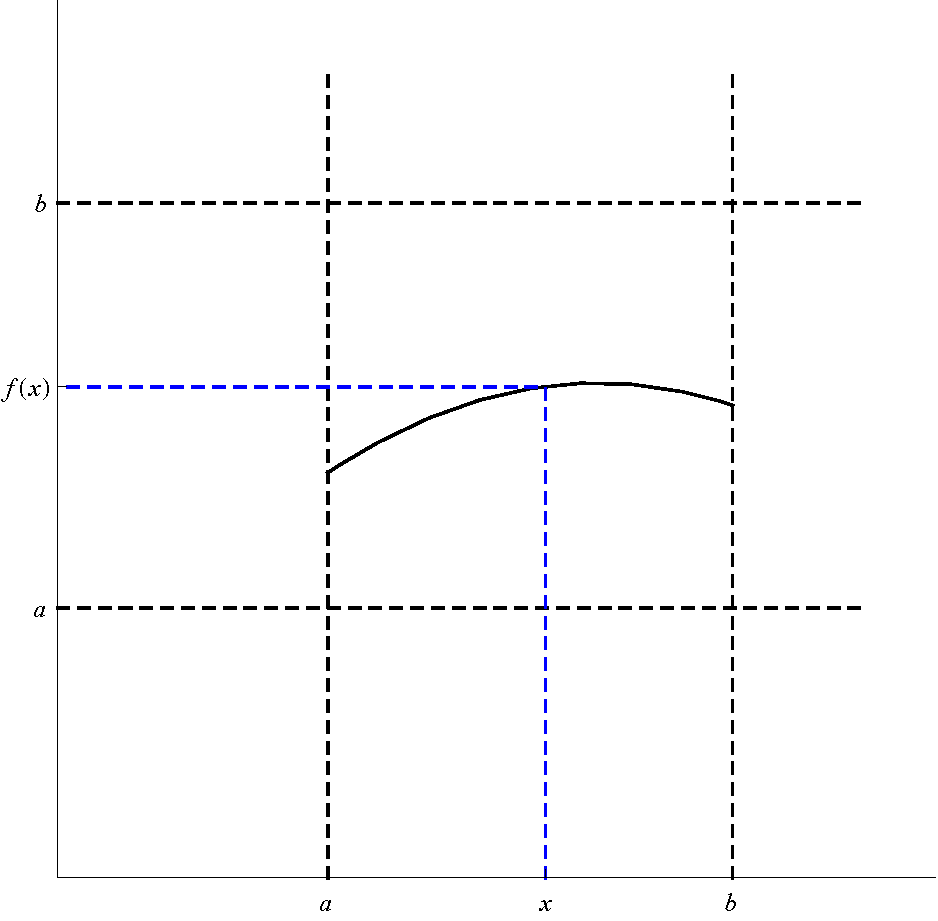
\includegraphics[width=0.6\textwidth]{files/budongdian.pdf}\\
      对满足条件的任意函数 $f(x)$, 注意到在左端点 $a$ 处由横纵坐标 $(a,f(a))$ 构成的长方形的横向边长是小于等于纵向边长的; 在右端点 $b$ 处由横纵坐标 $(b,f(b))$ 构成的长方形的横向边长是大于等于纵向边长的; 这样无论函数曲线的形状是什么样子, 只要是连续的, 就一定在 $[a,b]$ 中存在点 $c$, 它相应的长方形的横纵边长是相等的. 即 $f(c)=c$.
    \item 从分析学角度, 令 $g(x)=f(x)-x$\,. 显然 $g(a)\ge0,g(b)\le0$. 若 $g(a),g(b)$ 至少有一个为 0, $a,b$ 就是所求的 $c$ 点; 若 $g(a),g(b)$ 都不为 0, 由于两者异号, 根据介值定理 $(a,b)$ 上一定有一点 $g(c)=0$.
  \end{enumerate}
\end{proof}

\section{单侧极限相关定理证明}
\Cref{the:OneSideAndTwoSideLimit} 的\hypertarget{proof:OneSideAndTwoSideLimit}{证明}.
\begin{proof}
  \leavevmode

  \begin{itemize}
    \item 必要性. 从函数极限的任何一个定义来看, 若在整个邻域上满足条件自然在两侧都满足那些条件.
    \item 充分性. 从 $\varepsilon$-$\delta$ 式定义来看, 令 $\delta=\min\set{\delta_1,\delta_2}$ 即可. 从序列式定义来看, $\puncU{a}$ 上任何收敛的序列, 都可以由两边各自的所有收敛序列构成.
  \end{itemize}
\end{proof}

\section{指数函数对数函数相关证明}
\Cref{the:ExponentQTheorem} 的\hypertarget{proof:ExponentQTheorem}{证明}.
\begin{proof}
  \leavevmode

  设 $p=\frac{k}{n},q=\frac{l}{n}$. $k,l,n\in\Z,n\neq0,k<l$.
  \begin{itemize}
    \item 
      \begin{equation*}
	a^{p+q}=a^{\frac{k+l}{n}}=a^{\frac{k}{n}}\cdot a^{\frac{l}{n}}=a^p \cdot a^q\,.
      \end{equation*}
    \item 由于 $a>1$ 时, $a^{\frac{1}{n}}>1$. 所以 $\left( a^{\frac{1}{n}} \right)^k<\left( a^{\frac{1}{n}} \right)^l$.
  \end{itemize}
\end{proof}

对数运算律 \cref{the:LogOperations} 的\hypertarget{proof:LogOperations}{证明}.
\begin{proof}
  \leavevmode

  \begin{enumerate}
    \item 根据对数定义容易理解.
    \item 根据对数定义容易理解.
    \item 因为 $a^{b\log_a x}=x^b$, 两边取 $\log_a$ 对数\footnote{对一个等式两边可以同时取对数的原因是什么? 是因为对数是某定义域下的函数, 而函数的定义就是一个自变量对应一个值, 所以能够保证两个相等的量取了对数之后还是相等的.}.
    \item 因为 $a^{\log_a x+\log_a y}=xy$, 两边取 $\log_a$ 对数.
    \item 在上一式中代换 $y\to-y$.
    \item 因为 $y^{\frac{\log_a x}{\log_a y}}=\left( a^{\log_a y} \right)^{\frac{\log_a x}{\log_a y}}=x$, 两边取 $\log_y$ 对数.
    \item 上一式把分母乘到右边.
  \end{enumerate}
\end{proof}

\section{导数证明}
\hypertarget{proof:PowerFunctionDerivatives}{}
\begin{proof}
  \begin{align*}
    \lim_{\Delta x\to 0}\frac{f(x+\Delta x)-f(x)}{\Delta x}&=\lim_{\Delta x\to 0}\frac{\frac{1}{(x+\Delta x)^m}-\frac{1}{x^m}}{\Delta x}\\
    &=\lim_{\Delta x\to 0}\frac{x^m-(x+\Delta x)^m}{\Delta x x^m (x+\Delta x)^m}\\
    &=\lim_{\Delta x\to 0}\frac{-\sum_{l=0}^{m-1}\binom{m}{l}x^{l-m}(\Delta x)^{m-l-1}}{(x+\Delta x)^m}\\
    &=\frac{-\binom{m}{m-1}x^{m-1-m}}{x^m}\\
    &=-m x^{-(m+1)}
  \end{align*}
  注意到 $x$ 是求导数的基点, 故右端对差商函数求极限时自变量是隐含的 $x_1$, 不是 $x$.
\end{proof}

\hypertarget{proof:PowerFunctionGeneralDerivatives}{}
\begin{proof}
  \begin{align*}
    f'(x)&=\lim_{\Delta x\to 0}\frac{(x+\Delta x)^\mu}{\Delta x}\\
    &=\lim_{\Delta x\to0}\frac{x^\mu\left[ \left( 1+\frac{\Delta x}{x} \right)^\mu-1 \right]}{\Delta x}
  \end{align*}
  注意到上式中出现 $x\to0$ 过程中的等阶量 $(1+x)^\mu-1\sim \mu x$.
\end{proof}

\hypertarget{proof:Derivative_of_Composite_Functions}{}
\begin{proof}
  $g(f(x))$ 在 $x_0$ 点的导数按定义写为:
  \begin{equation*}
    \lim_{x\to x_0}\frac{g(f(x))-g(f(x_0))}{x-x_0}=\frac{g(f(x))-g(f(x_0))}{f(x)-f(x_0)}\frac{f(x)-f(x_0)}{x-x_0}\,.
  \end{equation*}
  若两部分极限都存在则整体极限存在.
  先求第一部分的极限:
  $f(x)$ 在 $x_0$ 点连续, 故
  \begin{equation*}
    \lim_{x\to x_0} f(x)=f(x_0)\,.
  \end{equation*}
  设差商函数 $\psi(y)=\frac{g(y)-g(y_0)}{y-y_0}$.
  $g(y)$ 在 $y_0=f(x_0)$ 可导, 即差商函数 $\psi(y)$ 在 $y_0$ 有极限 $g'(y_0)$.
  \begin{equation*}
    \lim_{y\to y_0} \psi(y)=g'(y_0)\,.
  \end{equation*}
  按照复合函数的极限运算律可知, 复合函数 $\psi(f(x))$ 在 $x_0$ 点的极限存在:
  \begin{equation*}
    \lim_{x\to x_0}\psi(f(x))=\lim_{x\to x_0}\frac{g(f(x))-g(f(x_0))}{f(x)-f(x_0)}=g'(y_0)=g'(f(x_0))\,.
  \end{equation*}
  因此第一部分极限存在. 已知 $f(x)$ 在 $x_0$ 点可导, 故
  \begin{equation*}
    \varphi'(x_0)=g'(f(x_0))f'(x_0)\,.
  \end{equation*}
\end{proof}

\hypertarget{proof:inverse_func_derivative}{}
\begin{proof}
  因为函数在 $x_0$ 点连续, 所以反函数在 $y_0$ 点连续.\\
  因此, $\lim_{y\to y_0}\psi(y)=\psi(y_0)=x_0$.
  \begin{align*}
    \lim_{y\to y_0}\frac{\psi(y)-\psi(y_0)}{y-y_0}\\
    \intertext{做替换 $x=\psi(y)$, 得到}
    &=\lim_{x\to x_0}\frac{x-x_0}{\varphi(x)-\varphi(x_0)}\\
    &=\lim_{x\to x_0}\frac{1}{\frac{\varphi(x)-\varphi(x_0)}{x-x_0}}\\
    &=\frac{1}{\varphi'(x_0)}
  \end{align*}
\end{proof}

\hypertarget{proof:deriv:Leibniz_formula}{}
\begin{proof}
  数学归纳法证明.\\
  已知, $n\to1$ 时 Leibniz 公式就是乘积求导公式, 显然成立.\\
  设 $n\to n-1$ 时公式成立, 即
  \begin{equation*}
    (uv)^{(n-1)}=\sum_{k=0}^{n-1}\binom{n-1}{k}u^{(k)}v^{(n-1-k)}\,.
  \end{equation*}
  则, $n\to n$ 时, 
  \begin{align*}
    (uv)^{(n)}&=\Big( (uv)^{(n-1)} \Big)'=\sum_{k=0}^{n-1}\binom{n-1}{k}\Big( u^{(k+1)}v^{(n-1-k)}+u^{(k)}v^{(n-k)} \Big)\\
    &=\sum_{k=0}^{n-1}\binom{n-1}{k}u^{(k+1)}v^{(n-1-k)}+\sum_{k=0}^{n-1}\binom{n-1}{k}u^{(k)}v^{(n-k)}
    \intertext{第一项中代换 $k+1=j$,}
    &=\sum_{j=1}^{n}\binom{n-1}{j-1}u^{(j)}v^{(n-j)}+\sum_{k=0}^{n-1}\binom{n-1}{k}u^{(k)}v^{(n-k)}\\
    &=\binom{n-1}{0}u^{(0)}v^{(n)}+\sum_{k=1}^{n-1}\left[ \binom{n-1}{k-1}+\binom{n-1}{k} \right]u^{(k)}v^{(n-k)}+\binom{n-1}{n-1}u^{(n)}v^{(0)}\,,
  \end{align*}
  由于 $\binom{n}{k}=\binom{n-1}{k-1}+\binom{n-1}{k}$, 证得 $n\to n$ 时公式也成立.
\end{proof}
\section{定积分相关证明}
\hypertarget{proof:IntegratableBoundary}{}
\begin{proof}
  反证法.
  若 $f$ 无界, 则至少在一个子区间 $[x_{j-1},x_j]$ 上面无界.
  另一方面, $f$ 可积, 说明:
  \begin{align*}
    &\Any\varepsilon>0,\Exists\delta>0,\Any P\text{ that }\abs{P}<\delta\text{ and }\xi,\\
    &\abs{\sigma(f,P,\xi)-I}<\varepsilon\,.
  \end{align*}
  从而以下结果应该对任意 $\xi$ 恒成立:
  \begin{align*}
    &\abs{\sigma(f,P,\xi)}<\abs{I}+\varepsilon.\\
    &\abs{\abs{\sum_{i\ne j}^{}f(\xi_i)\Delta x_i}-\abs{f(\xi_j)\Delta x_j}}<\abs{\sum_{i}^{}f(\xi_i)\Delta x_i}<\abs{I}+\varepsilon,\\
    &\abs{f(\xi_j)\Delta x_j}<\abs{\sum_{i\ne j}^{}f(\xi_i)\Delta x_i}+\abs{I}+\varepsilon\,.
  \end{align*}
  若 $f$ 在 $[x_{j-1},x_j]$ 上无界, 上式中最后的结果不可能对任意 $\xi_j$ 都成立. 得出矛盾.
\end{proof}
\hypertarget{proof:NewtonLeibnizFormula}{}
\begin{proof}
  对 $[a,b]$ 的任意一个分割 $P$, 根据 Lagrange 定理可以把 $F(b)-F(a)$ 写成积分和的形式:
  \begin{equation*}
    F(b)-F(a)=\sum_{i}^{} (F(x_i)-F(x_{i-1}))=\sum_{i}^{} f(\eta_i)\Delta x_i
  \end{equation*}
  其中 $\eta_i$ 是按照 Lagrange 定理所确定的一点. $\eta$ 是相应于 $P$ 的一组特别选定的标志点.
  $f$ 在 $[a,b]$ 上一致连续.
  因此, 对 $\Any \varepsilon>0,\Exists \delta>0$, 只要 $\abs{x_1-x_2}<\delta$, 就有 $\abs{f(x_1)-f(x_2)}<\varepsilon$.
  只要 $\abs{P}<\delta$, 一致连续性的结果就可以应用在相应于 $P$ 分割的两组标志点 $\xi$ 和 $\eta$ 上, 其中 $\xi$ 是任意选择的标志点组, $\eta$ 是如上所述满足积分和为 $F(b)-F(a)$ 的标志点组. 推出任意的积分和 $\sigma(f,P,\xi)$ 与特定的积分和 $\sigma(f,P,\eta)$ 的差别在 $\varepsilon$ 阶.
  \begin{align*}
    \abs{\sigma(f,P,\xi)-(F(b)-F(a))}&=\abs{\sum_{i}^{}(f(\xi_i)-f(\eta_i))\Delta x_i}\\
    &<\sum_{i}^{}\abs{f(\xi_i)-f(\eta_i)}\Delta x_i\\
    &<(b-a)\varepsilon
  \end{align*}
  这就证明了, 对任意的 $\abs{P}<\delta$ 的 $P$, 无论 $\xi$ 怎么取, 积分和都在 $F(b)-F(a)$ 的 $\varepsilon$ 邻域内, 从而定积分值就是它.
\end{proof}
\hypertarget{proof:ArcLength}{}
\begin{proof}
  证明 $\rho,\sigma$ 在 $\abs{P}\to0$ 时有共同极限, 即证明: $\lim_{\abs{P}\to0}\rho-\sigma=0$.
  \begin{align*}
    \abs{\rho-\sigma-0}\le\sum_{i}^{}\abs{\sqrt{(x'(\tau_i))^2+(y'(\tau'_i))^2}-\sqrt{(x'(\tau_i))^2+(y'(\tau_i))^2}}\Delta t_i
  \end{align*}
  因为
  \begin{equation*}
    \abs{\sqrt{A^2+B^2}-\sqrt{A^2+C^2}}\le\abs{B-C},\quad \Any A,B,C\in\R,
  \end{equation*}
  得到
  \begin{equation*}
    \abs{\rho-\sigma}\le\sum_{i}^{}\abs{y'(\tau_i)-y'(\tau'_i)}\Delta t_i
  \end{equation*}
  因 $y'(t)$ 在 $[\alpha,\beta]$ 上有一致连续性, 对 $\Any \varepsilon>0,\Exists \delta>0,$ 只要 $\abs{\tau-\tau'}<\delta$ 就有 $\abs{y'(\tau)-y'(\tau')<\varepsilon}$. 只要取 $\abs{P}\delta$ 就有
  \begin{equation*}
    \abs{\rho-\sigma}\le\varepsilon(\beta-\alpha).
  \end{equation*}
  因此 $\rho,\sigma$ 有相同极限.
\end{proof}

\chapter{一些数学知识}
\section{等比数列}
等比数列 ${a_n}\,,n\in\N^+$ 的前 $n$ 项和公式为
\begin{equation*}
  S_n=a_1+a_2+\cdots+a_n=
  \begin{cases}
    \frac{a_1(1-q^n)}{1-q}\,,&(q\neq1)\,;\\
    na_1\,,&(q=1)\,.
  \end{cases}
\end{equation*}
\begin{proof}
  \begin{align}
    S_n&=a_1+a_2+\cdots+a_n\nonumber\\
    &=a_1+a_1 q+a_1 q^2+\cdots+a_1 q^{n-1}\label{eqn:sumofgeometricprogression}
  \end{align}
  两边乘以 $q$ 得到
  \begin{equation*}
    qS_n=a_1 q+a_1q^2+\cdots+a_1q^{n}\,.
  \end{equation*}
  用 \cref{eqn:sumofgeometricprogression} 减去上式得到
  \begin{equation*}
    S_n=\frac{a_1\left( 1-q^n \right)}{1-q}\,.
  \end{equation*}
  上式显然不适用 $q=1$ 时.
  在 $q=1$ 时, 观察 $S_n$ 形式, 得到
  $S_n=na_1$\,.
\end{proof}
\section{多项式}
\subsection{Definition}
A polynomial is an expression consisting of variables (or indeterminates) and coefficients, that involves only the operations of addition, subtraction, multiplication, and non-negative integer exponents.

A polynomial in a single indeterminate can be written in the form
\begin{equation*}
  a_n x^n + a_{n-1}x^{n-1} + \dotsb + a_2 x^2 + a_1 x + a_0,
\end{equation*}
where $a_0, \ldots, a_n$ are numbers, and $x$ is indeterminate.
This can be expressed more concisely by using summation notation:
\begin{equation*}
  \sum_{i=0}^n a_i x^i
\end{equation*}

\subsection{Terminology}
A polynomial can either be zero or can be written as the sum of a finite number of non-zero \emph{terms}. Each term consists of the product of a number---called the \emph{coefficient} of the term---and a finite number of indeterminates, raised to integer powers. The exponent on an indeterminate in a term is called the \emph{degree} of that indeterminate in that term; the degree of the term is the sum of the degrees of the indeterminates in that term, and \emph{the degree of a polynomial} is the largest degree of any one term with nonzero coefficient. A term and a polynomial with no indeterminates are called respectively a \emph{constant term} and a \emph{constant polynomial}; the degree of a constant term and of a nonzero constant polynomial is 0. The degree of the zero polynomial (which has no term) is not defined.

Polynomials of small degree have been given specific names. A polynomial of degree zero is a \emph{constant polynomial} or simply a \emph{constant}. Polynomials of degree one, two or three are respectively \emph{linear polynomials}, \emph{quadratic polynomials} and \emph{cubic polynomials}. For higher degrees the specific names are not commonly used, although \emph{quartic polynomial} (for degree four) and \emph{quintic polynomial} (for degree five) are sometimes used.

The polynomial 0, which may be considered to have no terms at all, is called the \emph{zero polynomial}.

In the case of polynomials in more than one indeterminate, a polynomial is called \emph{homogeneous of degree n} if all its terms have degree n.

\subsection{Etymology}
\sq{polynomial} was made simply by replacing the Latin root \emph{bi-} with the Greek \emph{poly-} in the word \sq{binomial}, where the \emph{-nomial} part is possibily derived from Latin \emph{nomen} which means \sq{name}.

\section{有理函数}
In mathematics, a rational function is any function which can be defined by a rational fraction, i.e. an algebraic fraction such that both the numerator and the denominator are polynomials. The coefficients of the polynomials need not be rational numbers, they may be taken in any field \emph{K}. In this case, one speaks of a rational function and a rational fraction over \emph{K}.

\subsection{Definition}
A function $f(x)$ is called a rational function if and only if it can be written in the form
\begin{equation*}
  f(x) = \frac{P(x)}{Q(x)} 
\end{equation*}
 where $P$, and $Q$, are polynomials in $x$, and $Q$, is not the zero polynomial. The domain of $f$, is the set of all points $x$, for which the denominator $Q(x)$, is not zero.

\section{数理逻辑中的量化}
\label{sec:logicalquantification}
\subsection{Predicate and Propositional function}
In mathematics, a \emph{predicate} (谓词) is commonly understood to be a Boolean-valued function $P:X\to\set{\text{true,false}}$, which is called the predicate $P$ on set $X$. A predicate can also be discribed as a statement that may be true or false depending on the values of its variables (predicate variables).

A \emph{propositional function} in logic, is a statement expressed in a way that would assume the value of true or false when inputting a variable $x$. The propositional function is abstracted from predicates. 

As an example, for the predicate \dq{$x$ is hot}, the substitution of any entity for $x$ will produce a specific \emph{proposition} that can be described as either true or false, even though \dq{$x$ is hot} on its own has no value as either a true or false statement. However, when you assign $x$ a value, such as lava, the function then has the value true; while if you assign $x$ a value like ice, the function then has the value false.

Propositional functions are useful in set theory for the formation of sets.
In this case, a set is formed by a collection of elements or predicate variables $x$ for which a propositional function $P(x)$ is true.

\subsection{Domain of discourse}
In the formal sciences, \emph{the domain of discourse}\footnote{discourse: formal and orderly and usually extended expression of thought on a subject.} (论域), also called \emph{the universe of discourse} (论述全集) or simply \emph{universe}, is the set of entities over which certain variables of interest in some formal treatment may range. 

The term universe of discourse generally refers to the collection of objects being discussed in a specific discourse.

\subsection{Open sentence}
In mathematics, an \emph{open sentence} (开放句子, usually an equation or equality) is described as ``open'' in the sense that its truth value is meaningless until its variables are replaced with specific numbers, at which point the truth value can usually be determined (and hence the sentences are no longer regarded as ``open''). These possible replacement values are assumed to range over a subset of either the real or complex numbers, depending on the equation or inequality under consideration. The replacement values which produce a true-value equation or inequality are called \emph{solutions} of the equation or inequality, and are said to ``satisfy'' it.

In mathematical logic, an \emph{open formula} is a formula which contains free variables. Unlike closed formulas, which contain constants, non-closed formulas do not express propositions; they are neither true nor false. A formula is said to be satisfied by any object(s) such that if it is written in place of the variable(s), it will form a sentence expressing a true proposition. Any sentence which results from a formula in such a way is said to be a substitution instance of that formula.

\subsection{Quantification}
In language and logic, \emph{quantification} (量化) is a construct that specifies the quantity of specimens in the domain of discourse that apply to (or satisfy) an open sentence. A language element which generates a quantification is called a \emph{quantifier} (逻辑量词). The resulting expression is a quantified expression (量化了的表达式); and the predicate or propositional function is said to be quantified by the quantifier on the domain of discourse. Quantification is used in both natural languages and formal languages. Examples of quantifiers in English are \dq{for all, for some, many, few, a lot, and no}. In formal languages, quantification is a formula constructor that produces new formulas from old ones.

For example, $\Any x\in\R,x^2\ge0$ is a quantified expression. In other word, the predicate $x^2\ge0$ is quantified by the quantifier $\forall$ on the domain of discourse $x\in\R$.

The two fundamental kinds of quantification in predicate logic are \emph{universal quantification} and \emph{existential quantification}. The traditional symbol for the universal quantifier ``all'' is ``$\forall$'', and for existential quantifier ``exists'' is ``$\exists$''.

\subsection{Universal quantification}
In predicate logic, a \emph{universal quantification} is generated by a type of quantifier, a logical constant which is interpreted as ``given any'' or ``for all''.  It expresses that a propositional function can be satisfied by every member of a domain of discourse.
The universal quantifier is denoted by \dq{$\forall$}.

A quantified propositional function is a statement; thus, like statements, quantified propositional functions can be \emph{negated}.

An universally quantified propositional function has the following form:
\begin{equation*}
  \Any x\in X,P(x)\,.
\end{equation*}
Its negation is
\begin{equation*}
  \neg\Any x\in X,P(x)\,,
\end{equation*}
which means: It is not the case that, given any element $x$ in $X$, $P(x)$ is true. The statement is equivalent to say that there must be at least one element for which $P(x)$ is not true. Thus,
\begin{equation*}
  \Exists x\in X,\neg P(x)\,.
\end{equation*}

We can therefore conclude that: the negation of a propositional function's universal quantification is an existential quantification of that propositional function's negation; symbolically,
\begin{equation*}
  \neg\Any x\in X, P(x) \bideduce \Exists x\in X, \neg P(x)\,.
\end{equation*}

\subsection{Existential quantification}
In predicate logic, an \emph{existential quantification} is generated by a type of quantifier, a logical constant which is interpreted as ``there exists'' or ``there is at least one''. It expresses that a propositional function can be satisfied by at least one member of a domain of discourse.
The existential quantifier is denoted by ``$\exists$''.

Corresponding to the conclusion above, we have: the negation of a propositional function's existential quantification is a universal quantification of that propositional function's negation; symbolically,
\begin{equation*}
  \neg\Exists x\in X, P(x) \bideduce \Any x\in X, \neg P(x)\,.
\end{equation*}

\section{充分条件与必要条件}
当命题 \dq{若 A 则 B} 为真时:
\begin{itemize}
  \item A 称为 B 的充分条件 (sufficient condition). 因为由 A 可以 \dq{充分地} 推出 B.
  \item B 称为 A 的必要条件 (necessary condition). 因为要得到 A, B 是 \dq{必要的}, 但可能不是唯一必要的 (即充分的).
\end{itemize}

当 \dq{若 A 则 B} 与 \dq{若 B 则 A} 皆为真时, A 是 B 的充分必要条件 (necessary and sufficient condition), 同时,  B 也是 A 的充分必要条件.

对于陈述 \dq{A 是 B 的充分必要条件}, 
\begin{itemize}
  \item 它的充分性部分是 \dq{A 是 B 的充分条件}.
  \item 它的必要性部分是 \dq{A 是 B 的必要条件}.
\end{itemize}


\section{三角函数}
\subsection{三角函数关系式}
\begin{align*}
  &\tan(a-b)=\frac{\tan a-\tan b}{\tan a\tan b+1}\\
  &\tan 2x=\frac{2\tan x}{1-\tan^2 x}
\end{align*}
\subsection{反三角函数关系式}
\begin{align*}
  \arcsin y+\arccos y&=\frac{\pi}{2}\qquad(\text{因为\ }y=\sin x=\cos(\frac{\pi}{2}-x))\\
  \arctan y+\arccot y&=\frac{\pi}{2}\qquad(\text{因为\ }y=\tan x=\cot(\frac{\pi}{2}-x))
\end{align*}
\section{双曲函数}
\subsection{几何意义}
双曲函数 (hyperbolic functions) 是一类与三角函数类似的函数.
$(\cosh\alpha,\sinh\alpha)$ 与单位双曲线的关系见 \cref{fig:hyperbolic_functions}. 其中, $\alpha$ 是双曲角, 它等于 hyperbolic sector (图中红色部分) 面积的两倍.
\begin{figure}[htb]
  \centering
  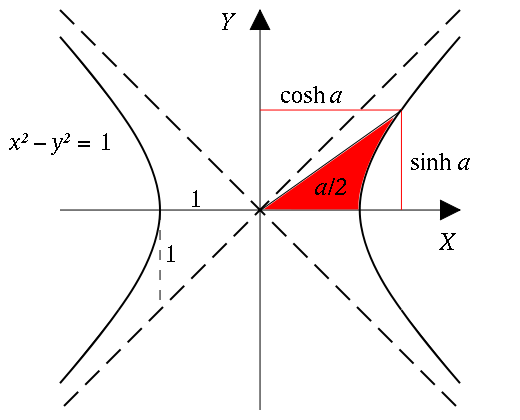
\includegraphics[width=0.5\textwidth]{files/hyperbolic_functions}
  \caption{}
  \label{fig:hyperbolic_functions}
\end{figure}
\subsection{代数表达式}
\begin{align*}
  \sinh x&=\frac{\e^x-\e^{-x}}{2}&\cosh x&=\frac{\e^x+\e^{-x}}{2}\\
  \tanh x&=\frac{\sinh x}{\cosh x}=\frac{\e^x-\e^{-x}}{\e^x+\e^{-x}}
  &\coth x&=\frac{\cosh x}{\sinh x}=\frac{\e^x+\e^{-x}}{\e^x-\e^{-x}}\\
  \sech x&=\frac{1}{\cosh x}
  &\csch x&=\frac{1}{\sinh x}
\end{align*}
\subsection{性质}
\begin{enumerate}
  \item 奇偶性:
    \begin{equation*}
      \sinh (-x)=-\sinh x\,,\qquad\cosh (-x)=\cosh x
    \end{equation*}
  \item 恒等式:
    \begin{align*}
      &\cosh^2 x-\sinh^2 x=1\\
      &\sech^2 x=1-\tanh^2 x\\
      &\csch^2 x=\coth^2 x-1
    \end{align*}
  \item 和角公式:
    \begin{align*}
      \sinh(x+y)&=\sinh x\cosh y+\cosh x\sinh y\\
      \cosh(x+y)&=\cosh x\cosh y+\sinh x\sinh y
    \end{align*}
  \item 二倍角公式:
    \begin{align*}
      \sinh 2x&=2\sinh x\cosh x\\
      \cosh 2x&=\cosh^2 x+\sinh^2 x=2\cosh^2-1=1+2\sinh^2 x
    \end{align*}
  \item 导数:
    \begin{align*}
      (\sinh x)'&=\cosh x\\
      (\cosh x)'&=\sinh x\\
      (\tanh x)'&=\sech^2 x\\
      (\coth x)'&=-\csch^2 x
    \end{align*}
  \item 与三角函数的关系:
    \begin{align*}
      \sinh x&=-\I\sin(\I x)\\
      \cosh x&=\cos(\I x)\\
      \tanh x&=-\I\tan(\I x)\\
      \coth x&=\I\cot(\I x)\\
      \sech x&=\sec (\I x)\\
      \csch x&=\I\csc (\I x)
    \end{align*}
\end{enumerate}
\subsection{三角函数与双曲函数的几何对比}
\begin{enumerate}
  \item 正弦同样是从x轴到曲线的半弦。
  \item 余弦同样是从y轴到曲线的半弦。
  \item 正切同样是过x轴上单位点(1,0)在曲线上的切线到终边的长度。
  \item 余切同样是从y轴与过终边和曲线交点的切线与y轴的交点和曲线连线之长度。
  \item 正割同样是在一个有正切和单位长的直角三角形上,但边不一样。
  \item 余割同样是y轴与过终边和曲线交点的切线与y轴的交点和原点之距离。
  \item 角的量值可以从 $-\infty$ 至 $+\infty$,但角度实际上只会介于0到2$\pi$之间,其余是同界角,再绕着圆旋转,故三角函数可以有周期。双曲角的量值也可以从 $-\infty$ 至 $+\infty$,但角度不会超过$\frac{\pi}{4}$,故无法如三角函数一样有周期性。
\end{enumerate}
\begin{figure}[htb]
  \centering
  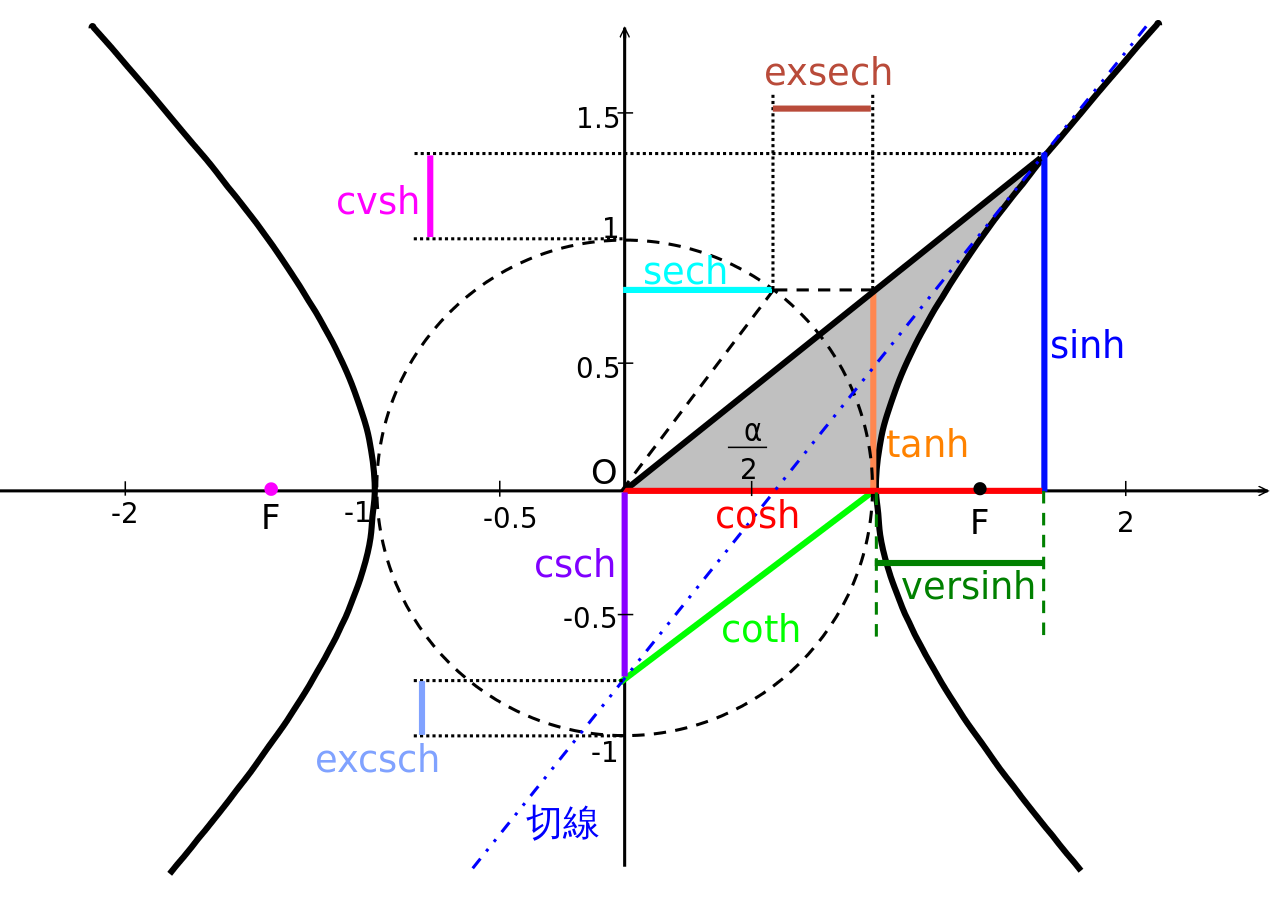
\includegraphics[width=0.45\textwidth]{files/hyperbolic_functions_all}
  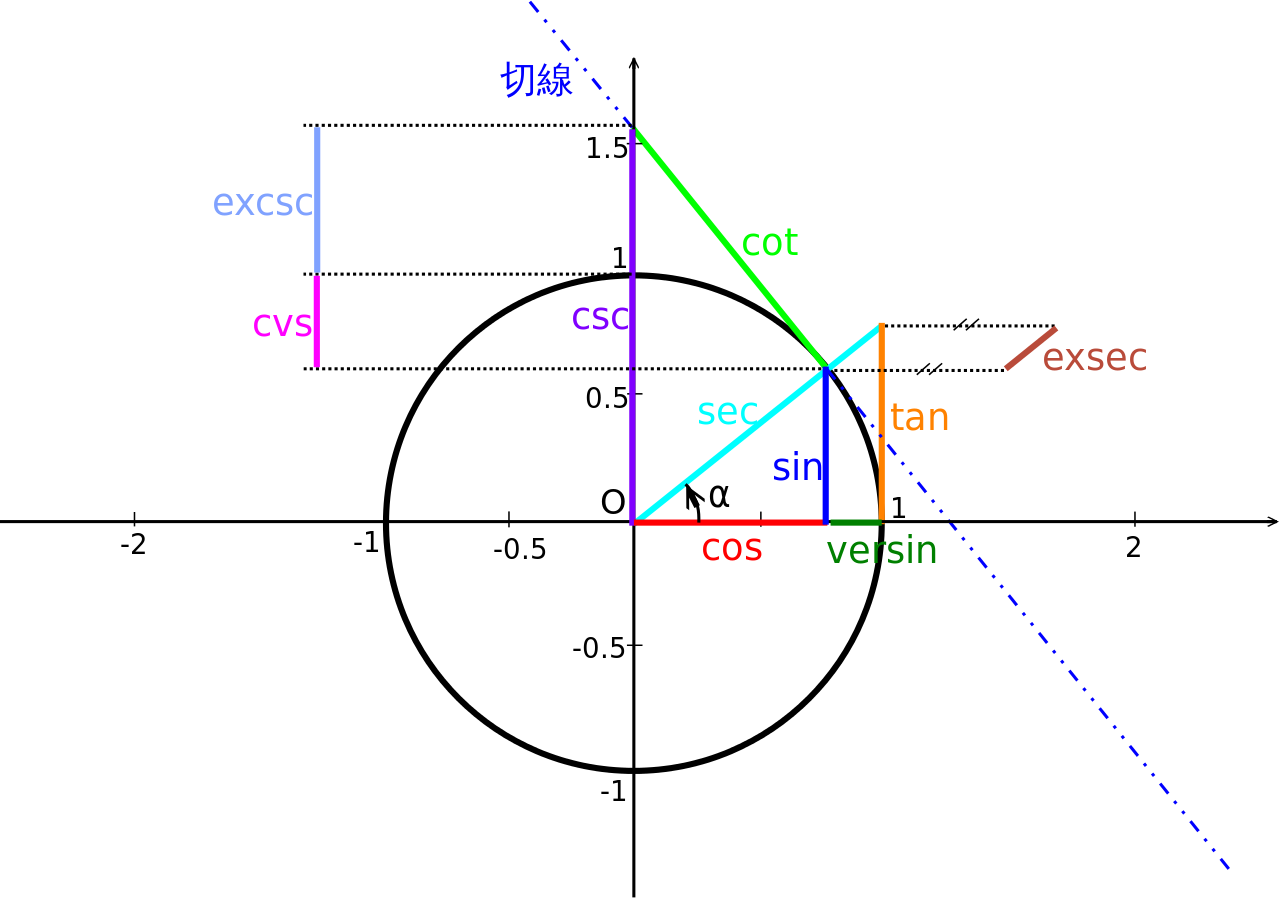
\includegraphics[width=0.45\textwidth]{files/trigonometric_functions_all}
  \caption{}
\end{figure}
\section{圆锥曲线}
\subsection{椭圆}
一般形式
\begin{equation*}
  Ax^2+Bxy+Cy^2+Dx+Ey+F=0
\end{equation*}
成为椭圆的条件: $B^2-4AC<0$. (为什么?)
设椭圆中心的位置是 $(x_c,y_c)$, 长轴与 $x$ 轴的转角为 $\theta$ (逆时针), 半长轴和半短轴分别是 $a,b$. (椭圆共 5 个自由度.) 
\begin{align*}
  A&=a^2(\sin\theta)^2+b^2(\cos\theta)^2\\
  B&=2(b^2-a^2)\sin\theta\cos\theta\\
  C&=a^2(\cos\theta)^2+b^2(\sin\theta)^2\\
  D&=-2Ax_c-By_c\\
  E&=-Bx_c-2Cy_c\\
  F&=Ax_c^2+Bx_cy_c+Cy_c^2-a^2b^2
\end{align*}
椭圆方程的一般形式和各参数可基于标准形式经过坐标变换推出.

\subsubsection{证明}
从椭圆的 canonical form
\begin{equation*}
  \frac{x^2}{a^2}+\frac{y^2}{b^2}=1
\end{equation*}
出发, 将椭圆逆时针旋转 $\theta$ 角度, 将中心平移至 $(x_c,y_c)$ 点, 即是任意的椭圆形式. 为此, 可以将坐标系反向顺时针旋转, 再平移; 利用两次操作时新旧坐标系的变换关系, 就得到了任意形式.

\begin{center}
  \begin{tikzpicture}
    [thick,x=2cm,y=2cm,scale=2]
    \coordinate (A) at (0.7,0.5);
    \coordinate (X) at (1,0);
    \coordinate (X') at (-30:1);
    \coordinate (O) at (0,0);
    \node [above right]at (A) {A};
    \draw[->,name path=xAxis] (-0.5,0)--(1,0);
    \draw[->,name path=yAxis] (0,-0.5)--(0,1);
    \draw[->,blue,name path=xAxis2] (0,0)--(-30:1);
    \draw[->,blue,name path=yAxis2] (0,0)--(60:1);
    \draw[dashed] (A)--(A|-0,0);
    \draw[dashed] (A)--(A-|0,0);
    \draw[dashed] (A)--($(0,0)!(A)!(-30:1)$);
    \draw[dashed] (A)--($(0,0)!(A)!(60:1)$);
    \path pic [draw=black,angle radius=0.5cm,angle eccentricity=1.4,"$\theta$"]{angle=X'--O--X};
  \end{tikzpicture}
\end{center}

对于平面上的点 $A$, 在原坐标系中表示为 $(x,y)$, 在旋转 $\theta$ 后的坐标系中表示为 $(x_1,y_1)$, 则变换关系为:
\begin{align*}
  x&=x_1\cos\theta+y_1\sin\theta\\
  y&=-x_1\sin\theta+y_1\cos\theta
\end{align*}
带入 canonical form 后得到了旋转坐标系中的椭圆方程, 也就是椭圆旋转任意角时的方程. 再将坐标系原点反向平移 $(x_c,y_c)$ 的距离, 即椭圆中心在新坐标系中的位置是 $(x_c,y_c)$, 得到任意点 $A$ 的坐标变换关系:
\begin{align*}
  x_1&=x_2-x_c\\
  y_1&=y_2-y_c
\end{align*}
再带入旋转坐标系内的椭圆方程, 就得到一般形式的椭圆方程.

\section{矢量分析}
\subsection{矢量的定义}
矢量是一个箭头,
具有长度和方向两个完备性质.
因此, 在座标系中, 默认起点在原点, 一组座标数字即可完全地表示矢量. 这是矢量分析的基础.

首先我们直觉地定义矢量由长度和方向两个性质构成, 代表一个这样大小和方向的某种操作. 因此两个矢量只要长度和方向相同, 就是同一个矢量 (同一个操作).

矢量表示为 $\mathbf{A}$ 或 $\vec{A}$, 它的长度表示为 $\abs{\mathbf{A}}$ 或 $A$. 直觉地想, 一个操作乘以一个数字应该是同方向的等比例伸缩后的操作, 因此定义一个矢量同方向的单位矢量为:
\begin{equation*}
  \hat{A}=\frac{\vec{A}}{A}\,,
\end{equation*}
因此, 一个矢量可以表示为
\begin{equation*}
  \vec{A}=A\hat{A}\,.
\end{equation*}
可以看作是大小和方向的乘积. (但注意所谓方向仍是一个单位矢量.)

由于物理量的测量值都是与基本单位比较得到的数值大小, 对于矢量物理量就把量纲和单位放在它的大小 $A$ 上面; 方向矢量 $\hat{A}$ 则表示它的方向.
\subsection{矢量的基本运算}
\subsubsection{数乘}
矢量的数乘
\begin{equation*}
  \vec{C}=b\vec{A}
\end{equation*}
自然是得到了一个同方向的长度是 $b$ 倍的矢量. 只不过注意 $b<0$ 时实际上是反方向.
\subsubsection{加法}
\begin{equation*}
  \vec{A}+\vec{B}=\vec{C}
\end{equation*}
得到了按照三角形定则或平行四边形法则所决定的 $\vec{C}$.
矢量的和按照三角形法则运算的原因仍然起源于直觉上对有向操作的理解. 即两个操作反向的那部分会抵消掉, 同向的那部分会叠加. 这也启发了用正交座标来表示矢量的分析方法.
\subsubsection{减法}
从逆运算的角度,
\begin{equation*}
  \vec{A}=\vec{C}-\vec{B}
\end{equation*}
求得的是能够与 $\vec{B}$ 按照三角形法则构成 $\vec{C}$ 的那个矢量 $\vec{A}$.

\section{线性映射}
Let $V$ and $W$ be vector spaces over the same field $K$. A function $f: V \to W$ is said to be a linear map if for any two vectors $\vec{x}$ and $\vec{y}$ in $V$ and any scalar $\alpha$ in $K$, the following two conditions are satisfied:
\begin{align*}
  &f(\vec{x}+\vec{y})=f(\vec{x})+f(\vec{y})\qquad(\text{additivity})\\
  &f(\alpha\vec{x})=\alpha f(\vec{x})\qquad(\text{homogeneity of degree 1})
\end{align*}
\chapter{扫描页}
\section{Toeplitz 数表和 Stolz 定理}
\hypertarget{scan:Toeplitz}{}
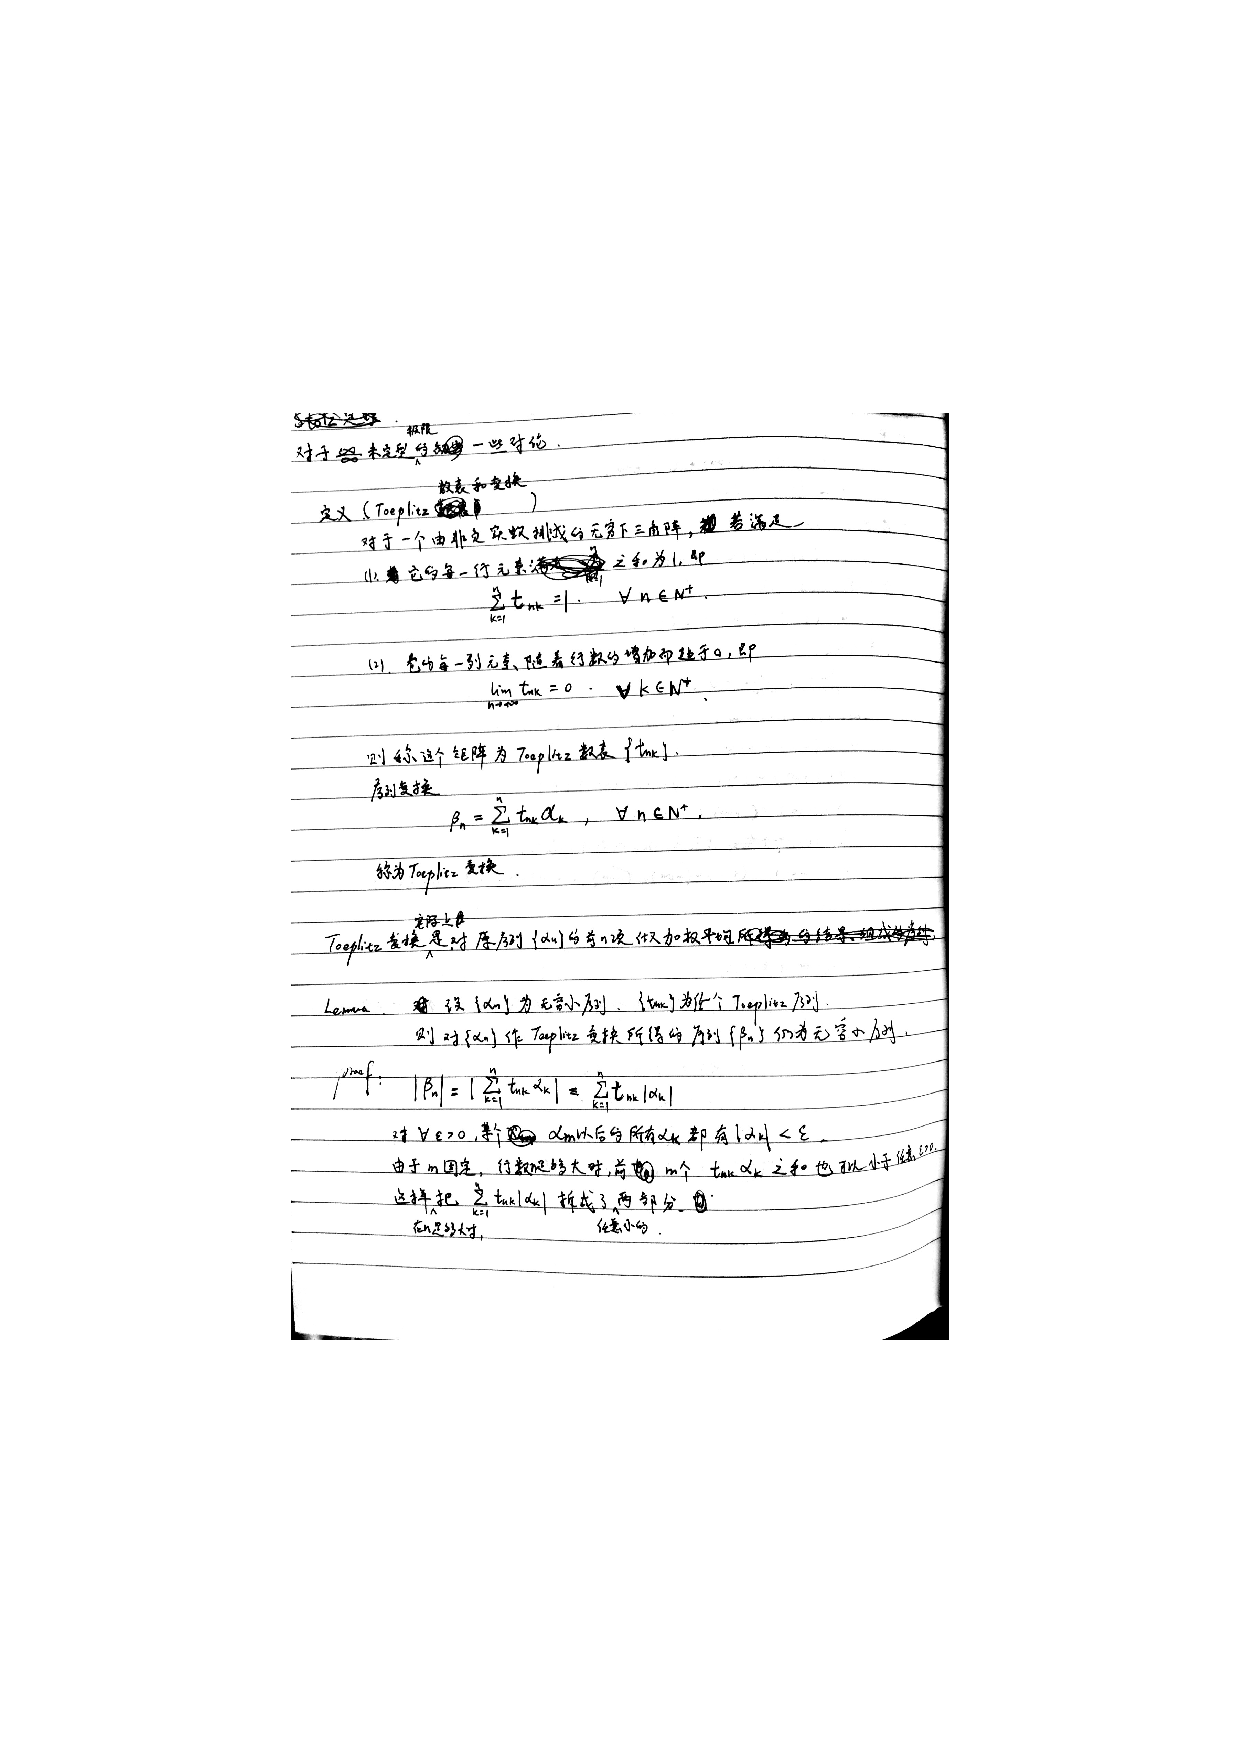
\includepdf[pages=-]{files/Toeplitz_Stolz.pdf}
\section{指数函数}
\hypertarget{scan:TwoLemmasForExponent}{}
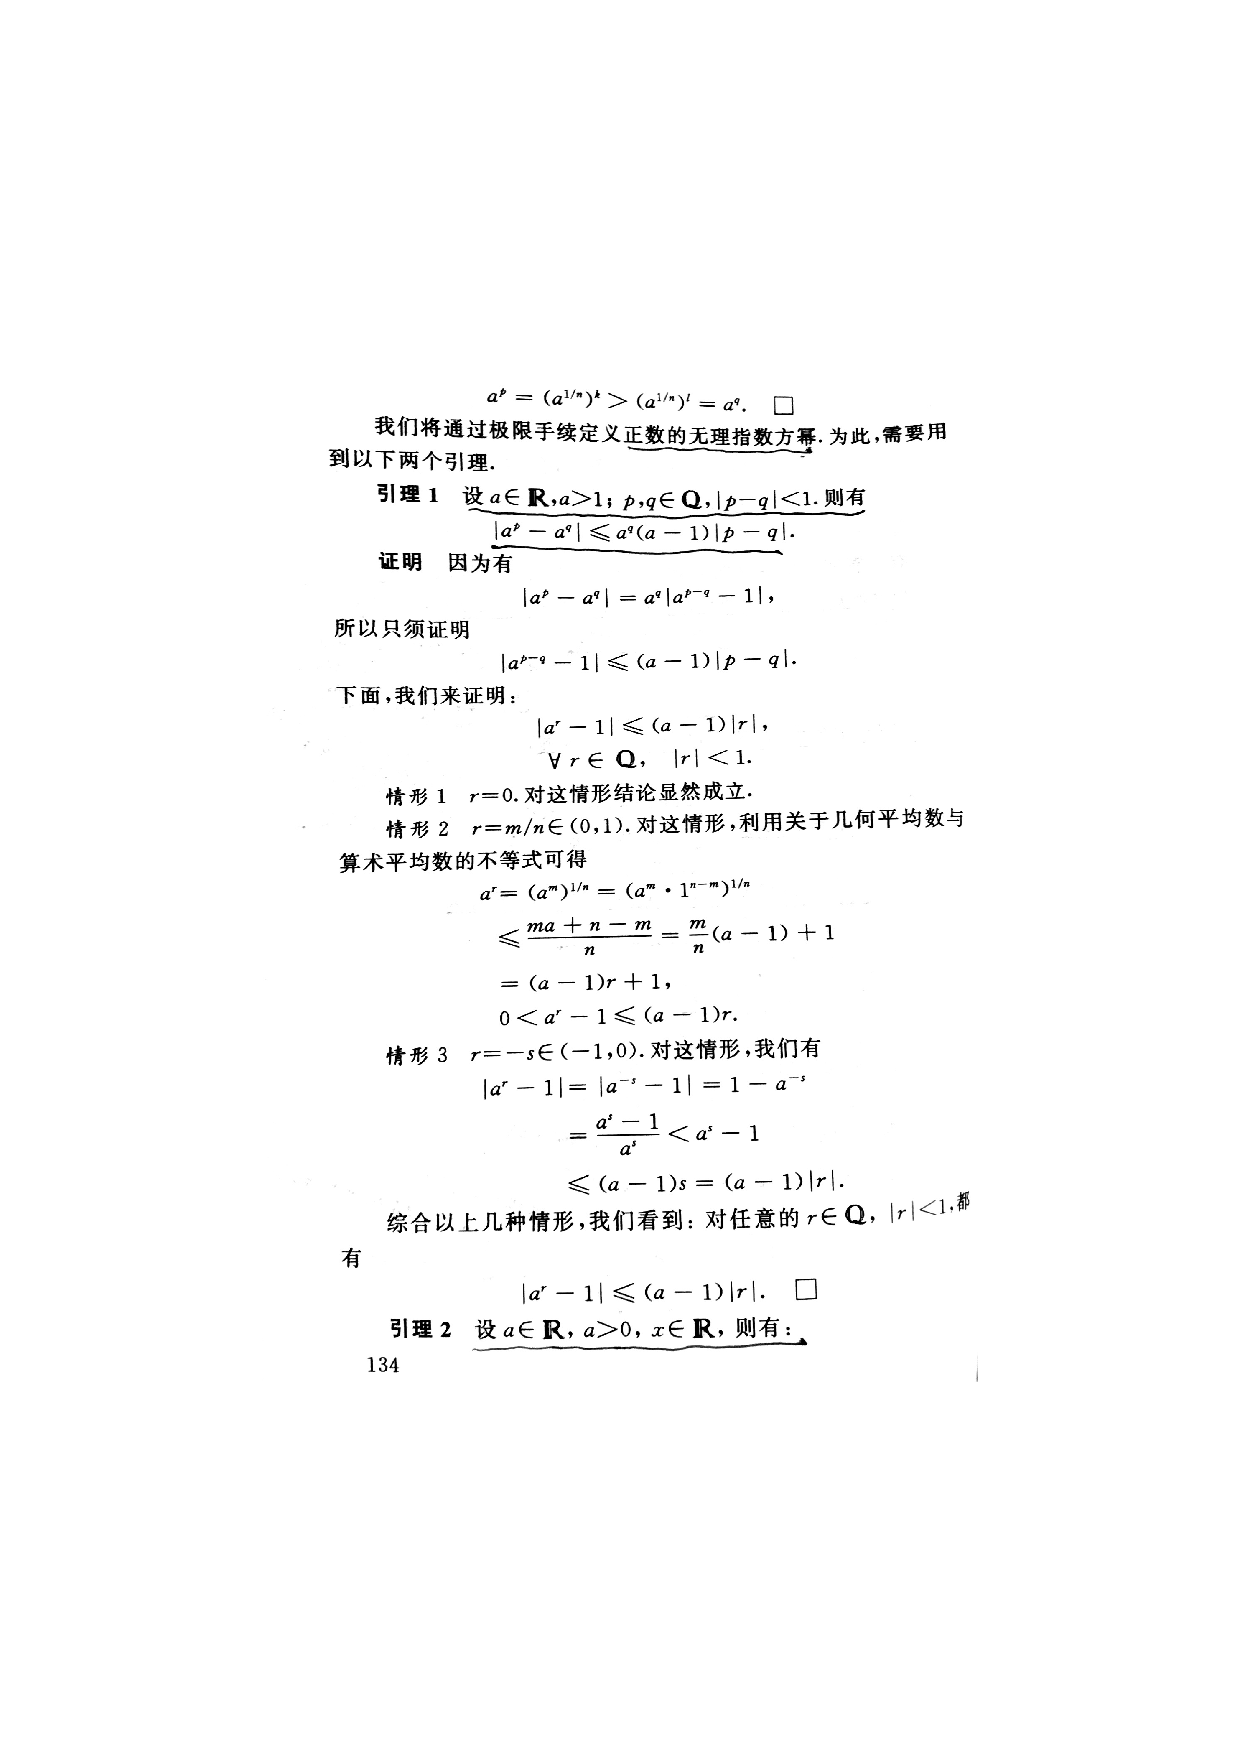
\includepdf[pages=-]{files/two_lemmas_exponent.pdf}

\hypertarget{scan:ExponentFunction}{}
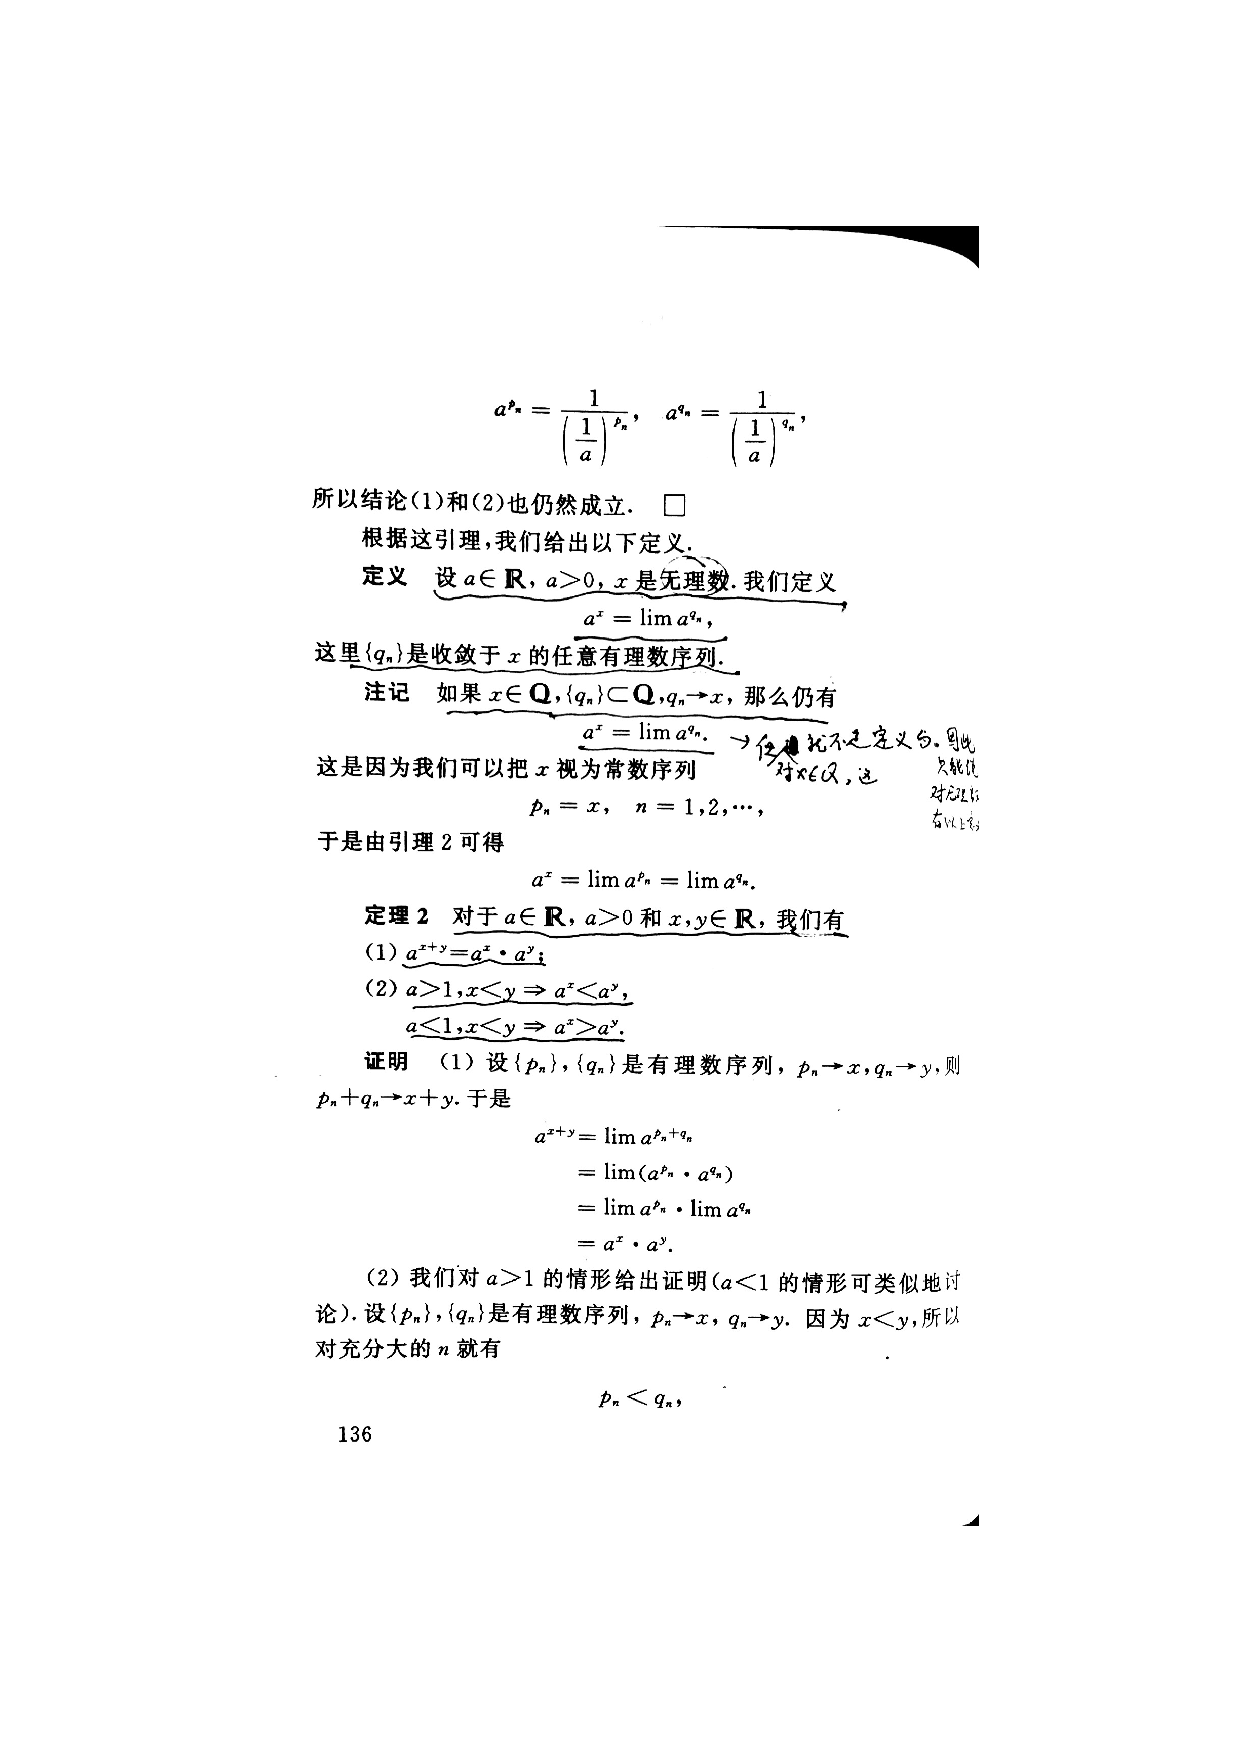
\includepdf[pages=-]{files/ExponentFunction.pdf}
\section{量阶}
\hypertarget{scan:ExponentFunctionPowerFunctionLogFunction}{}
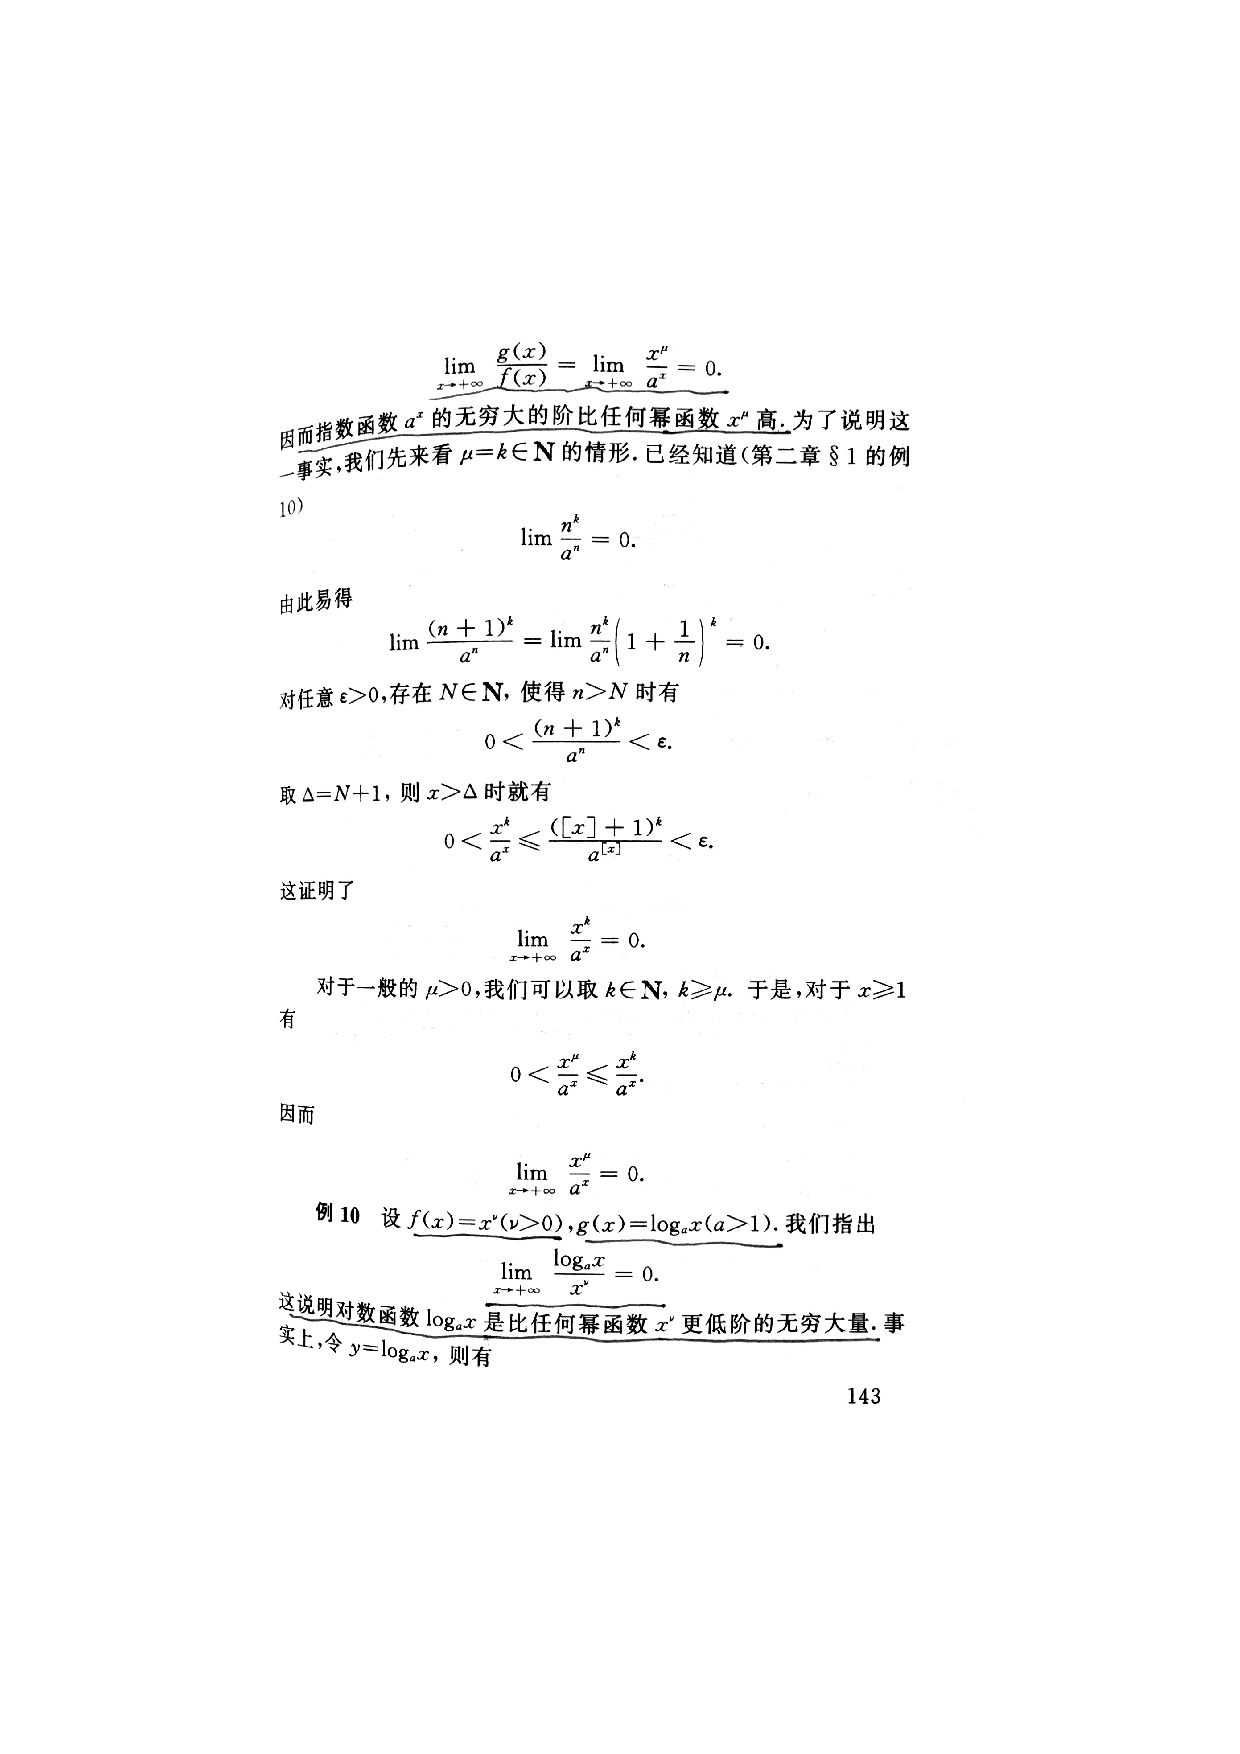
\includepdf[pages=-]{files/ExpPowerLog.pdf}
\section{重要极限}
\hypertarget{scan:ImportantLimit}{}
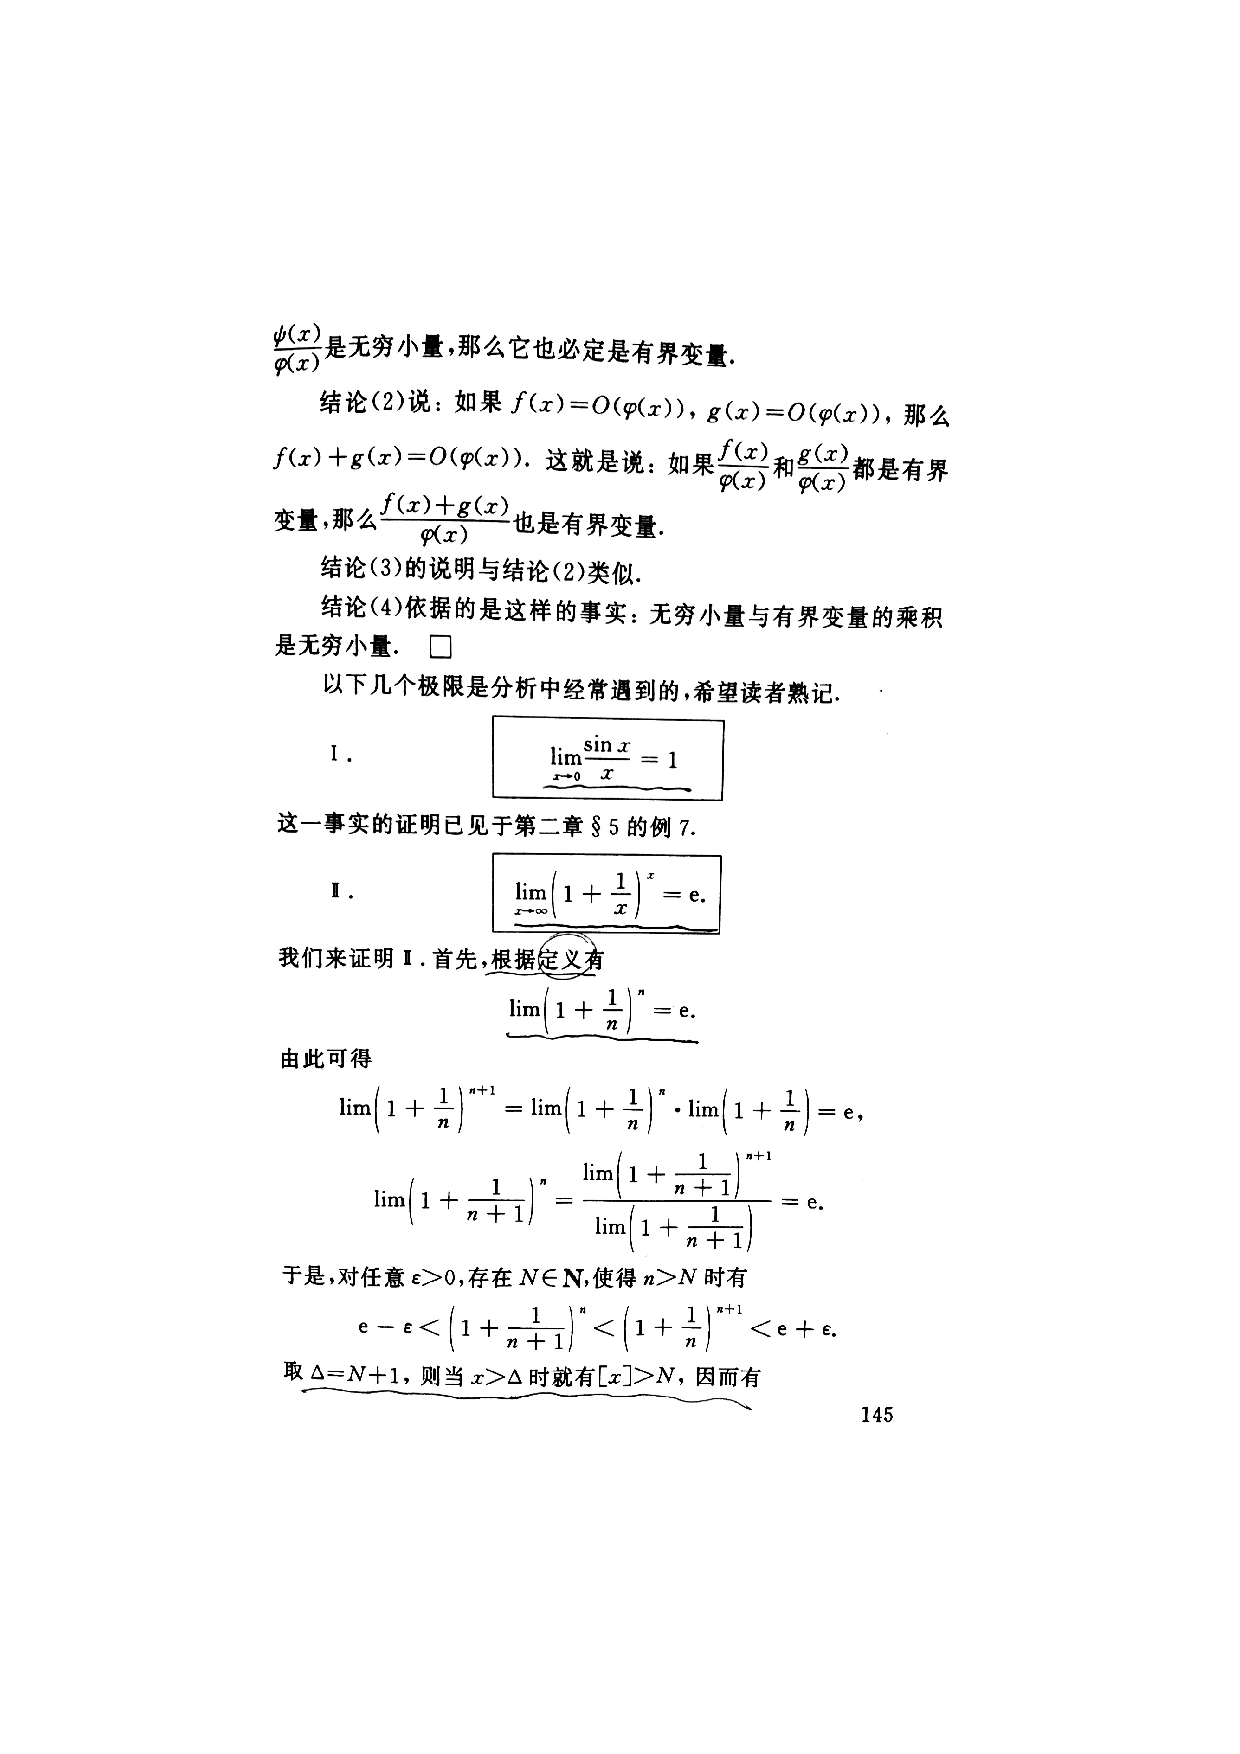
\includepdf[pages=-]{files/ImportantLimit.pdf}
\section{一致连续性}
\hypertarget{proof:yizhilianxuxingdingli}{}
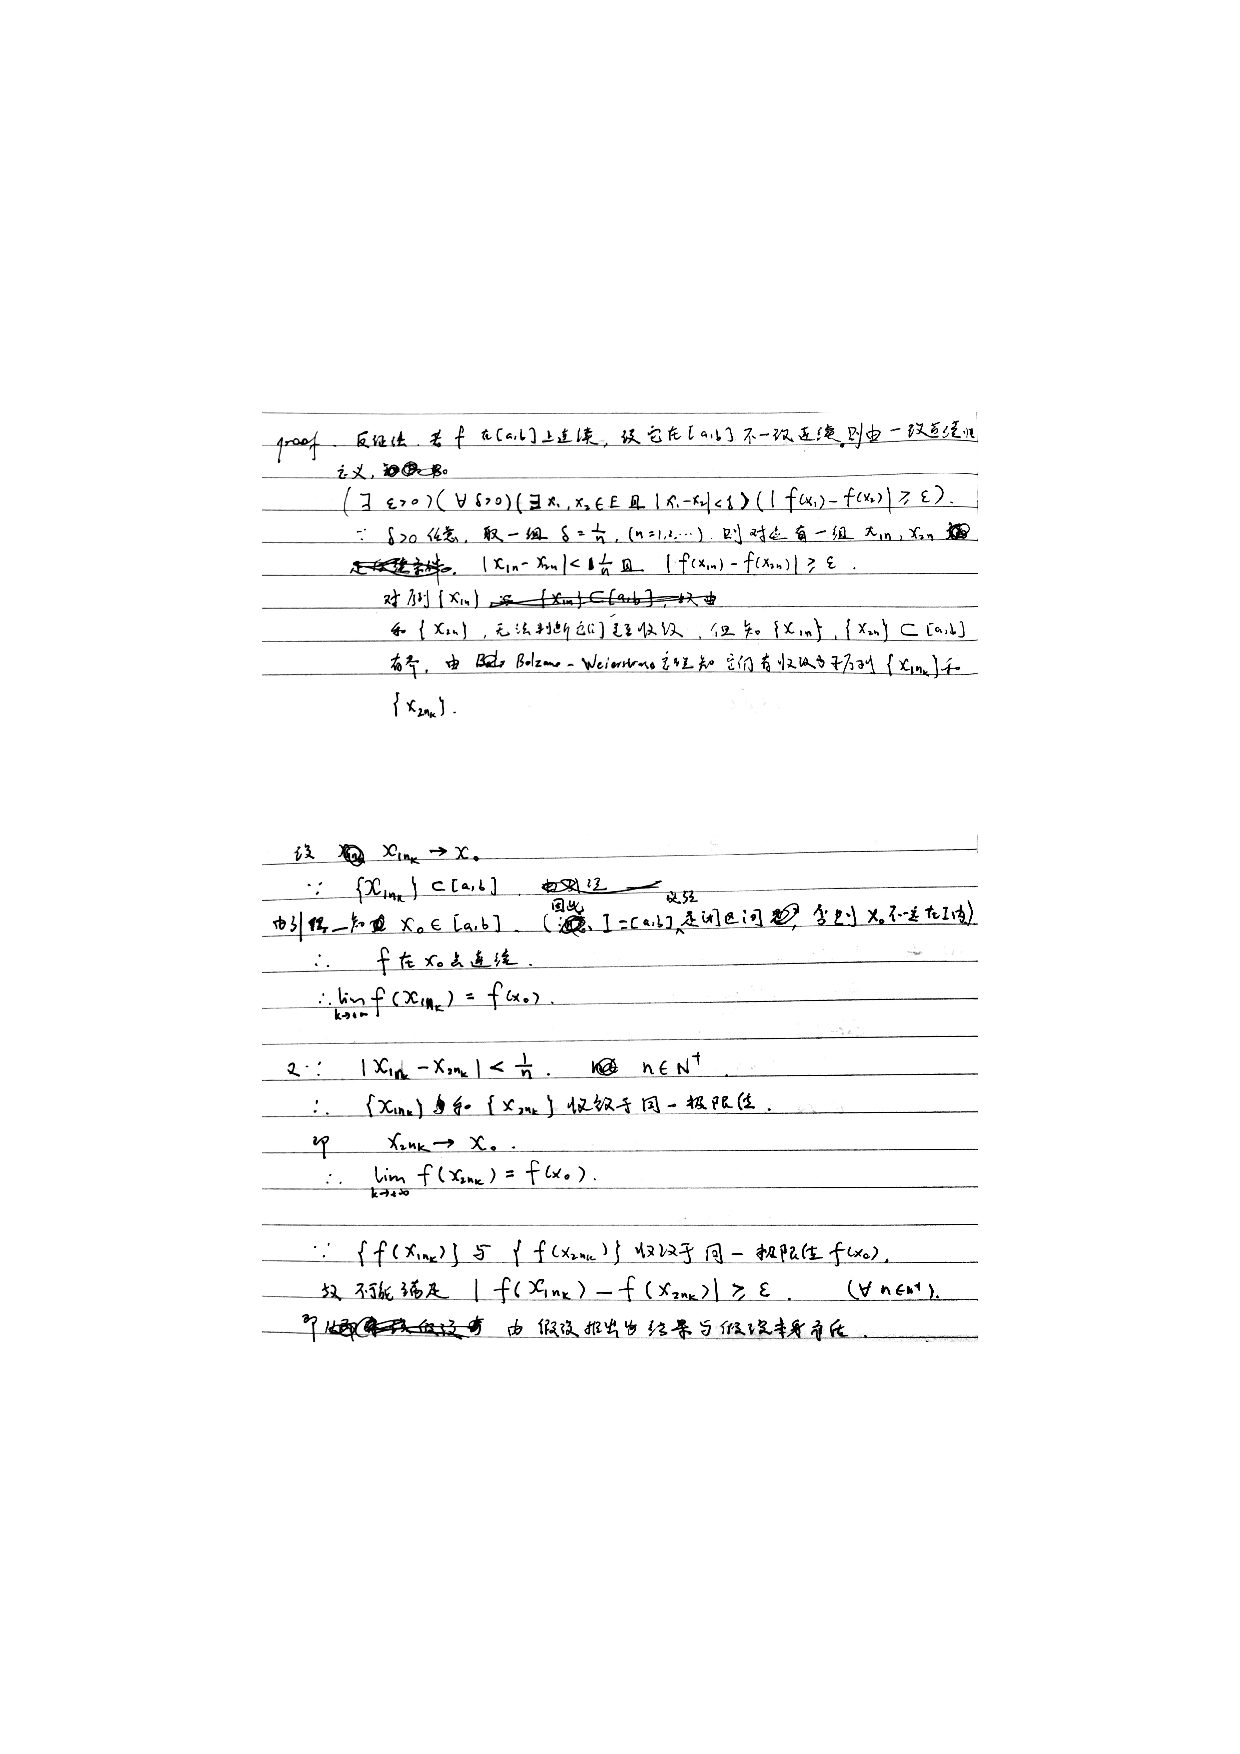
\includepdf[pages=-]{files/yizhilianxuxingdingli.pdf}
\hypertarget{proof:yizhilianxuxingTwoDefinitions}{}
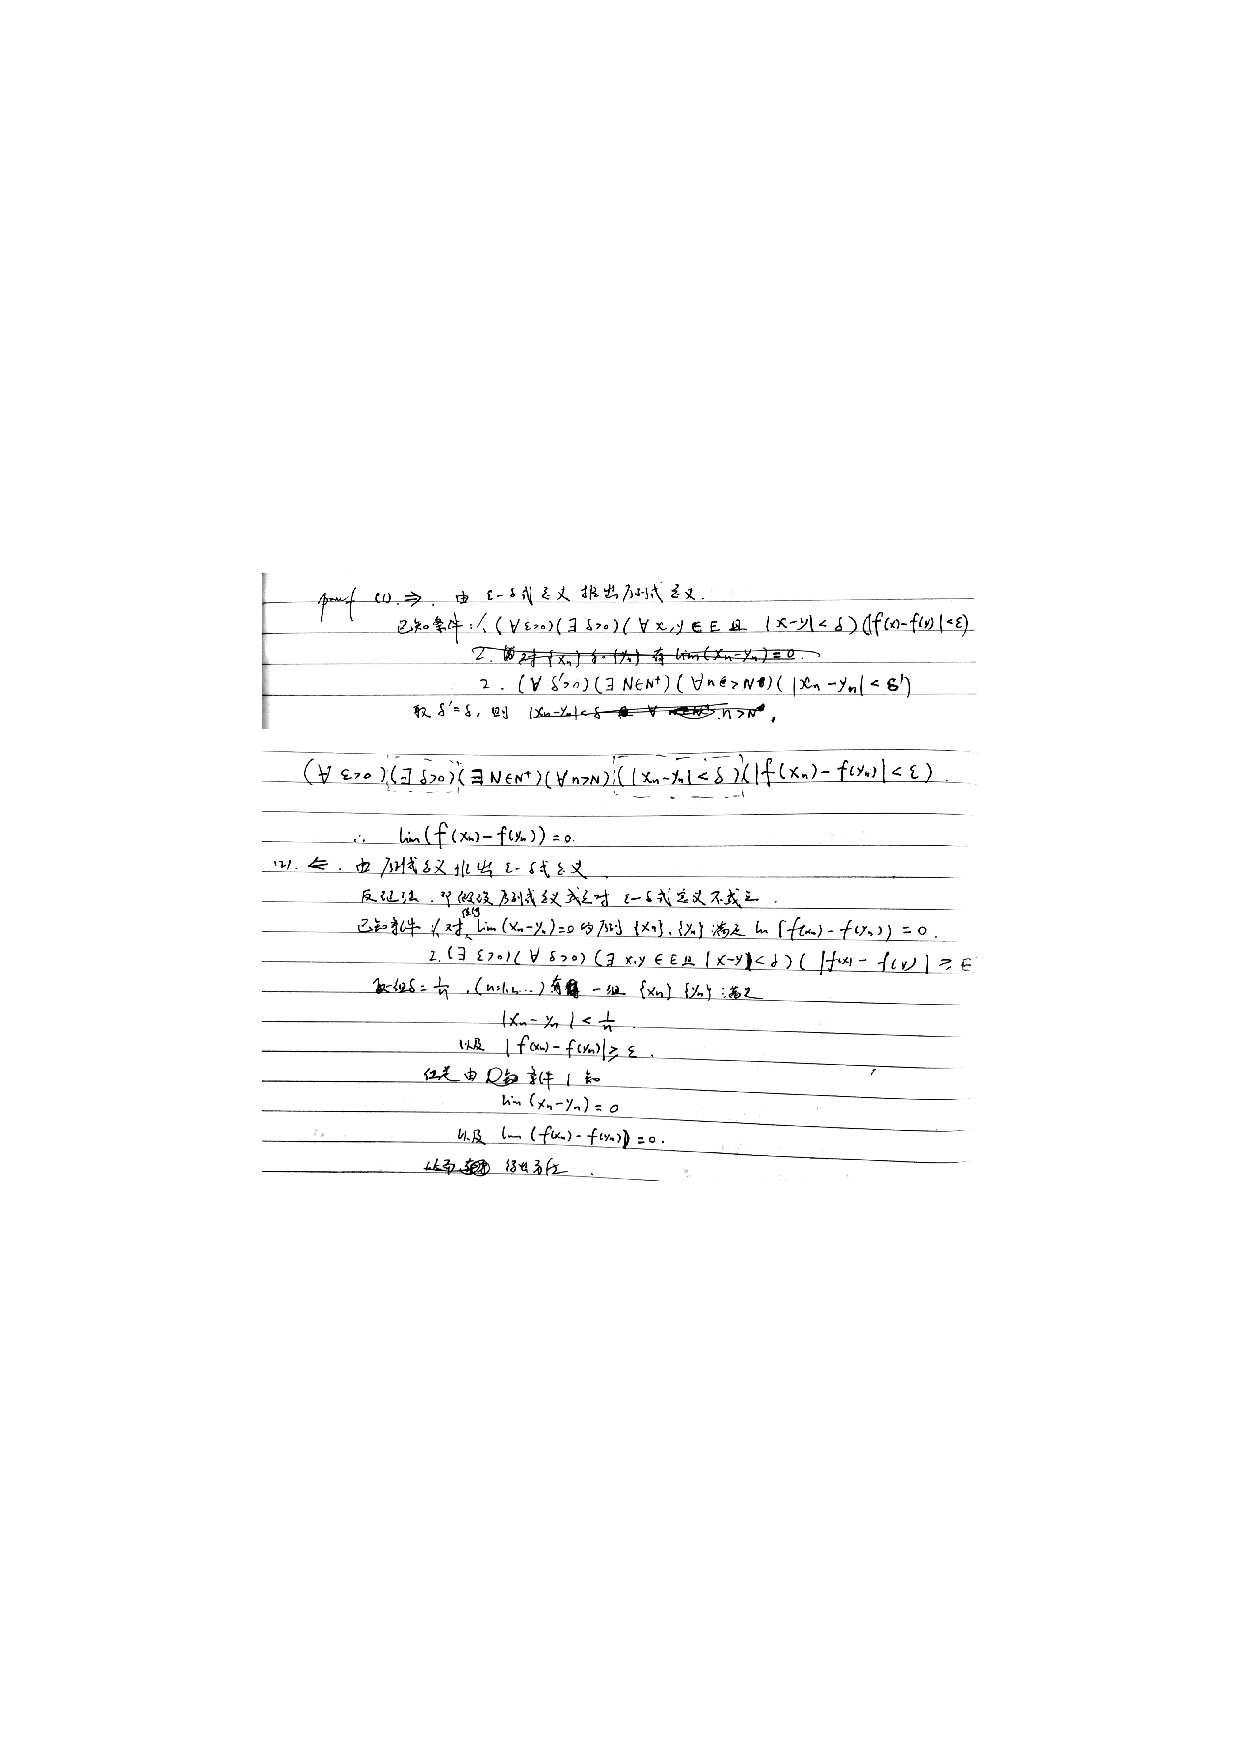
\includepdf[pages=-]{files/yizhilianxuxingTwoDefinitions.pdf}
\section{单调函数和反函数}
\hypertarget{scan:dandiao}{}
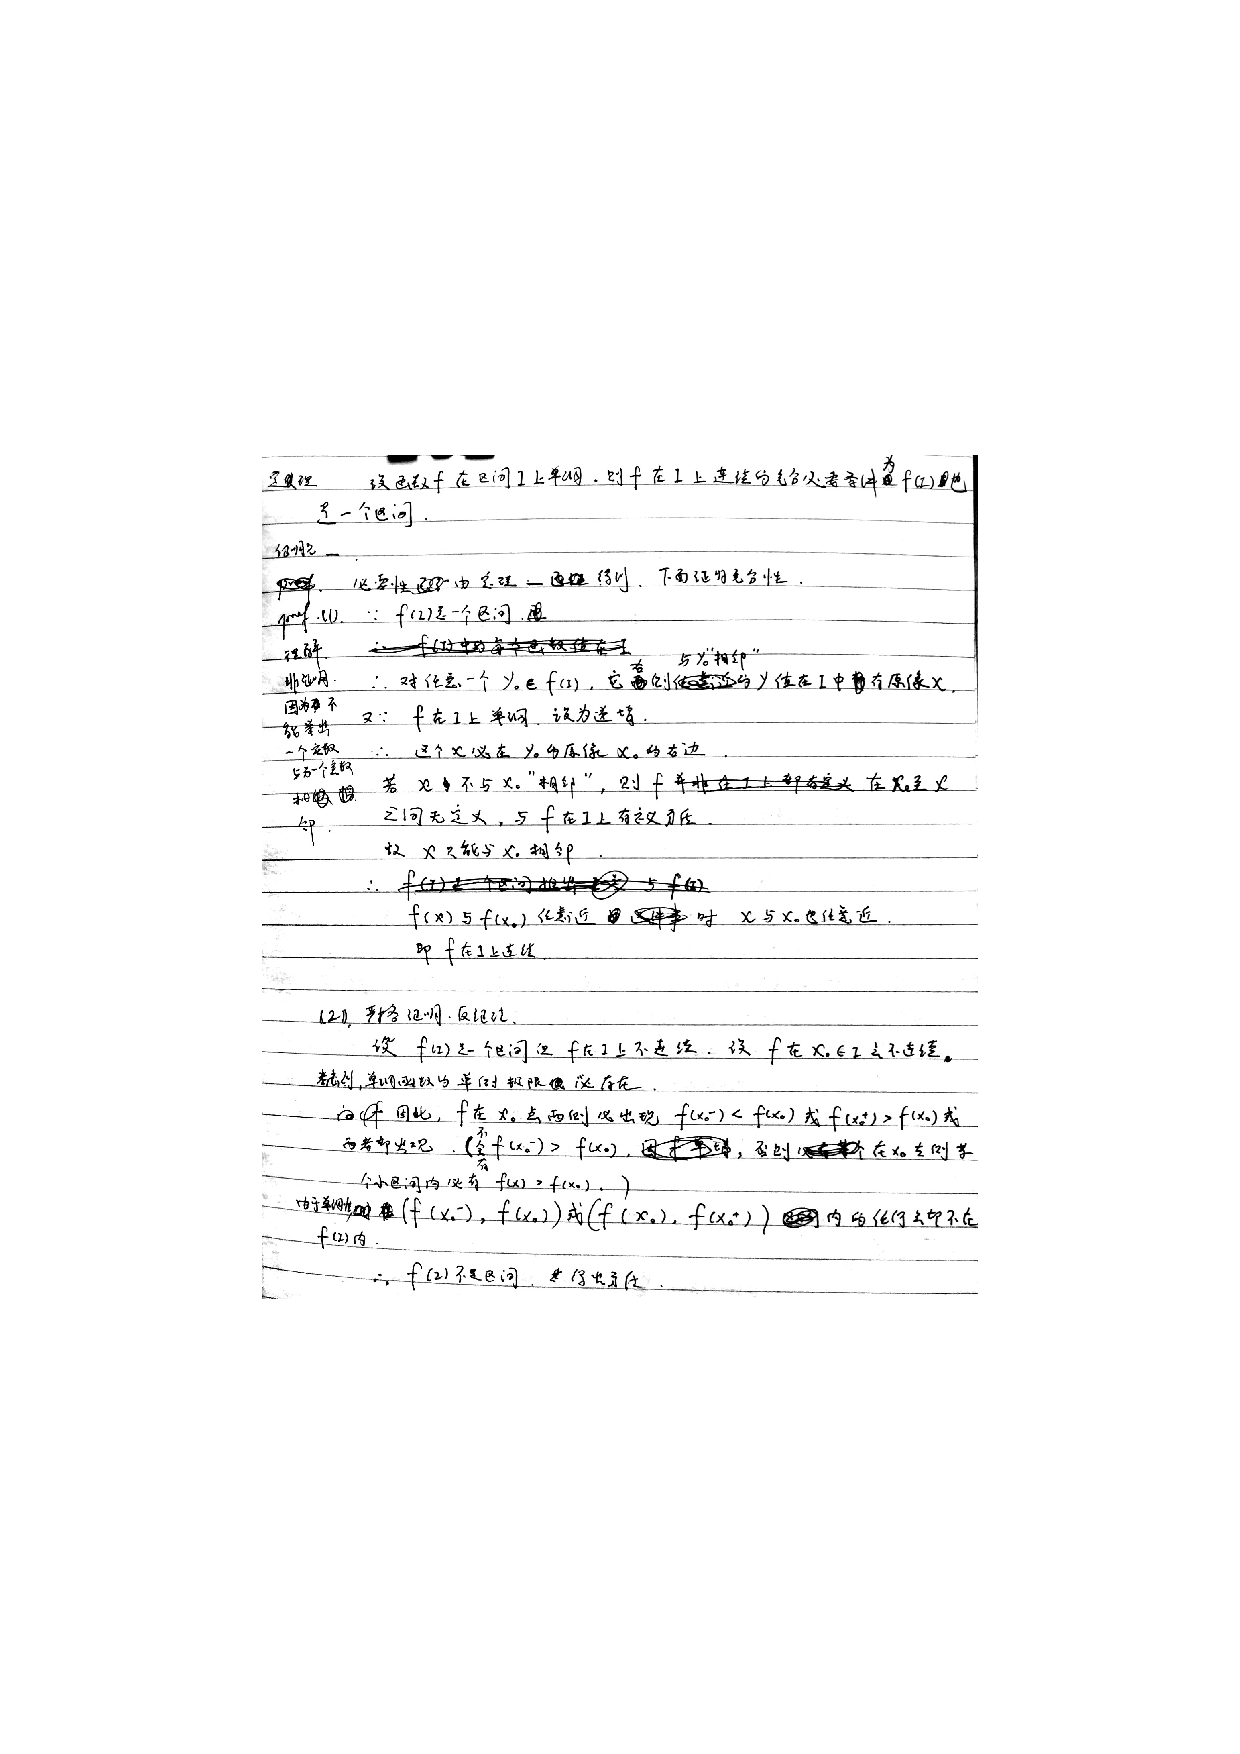
\includepdf[pages=-]{files/dandiao.pdf}
\section{定积分}
\hypertarget{scan:IntegratableHasBoundary}{}
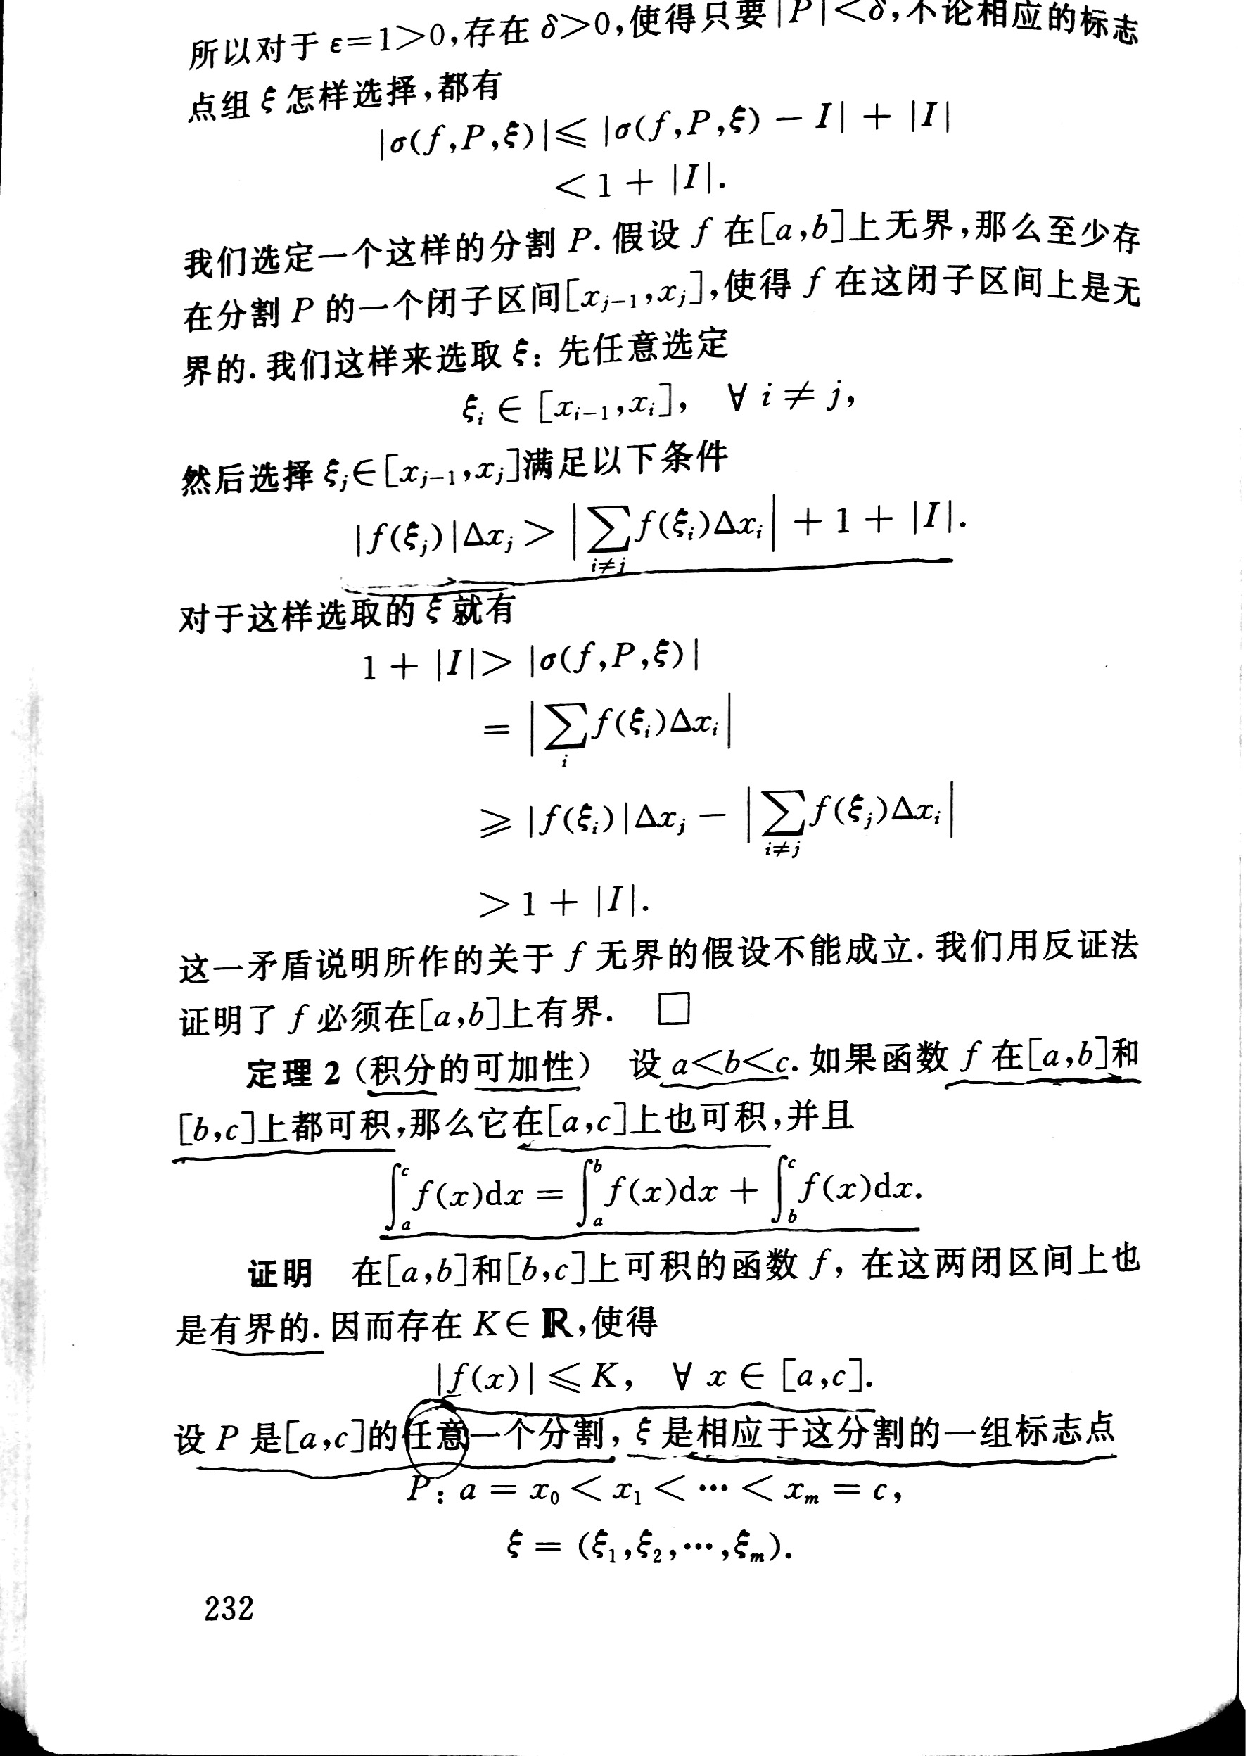
\includepdf[pages=-]{files/integratableHasBoundary.pdf}
\end{document}


